\documentclass[a4paper,11pt]{book}
% \documentclass[a4paper,twoside,11pt,titlepage]{book}
% Editar este fichero y rellenar los datos

% título y subtítulo del TFM en español
\newcommand{\tituloTFM}{Titulo del TFM}
\newcommand{\subtituloTFM}{Subtítulo del TFM}
% palabras clave en español
\newcommand{\palabrasClave}{palabra clave 1, palabra clave 2, \ldots, palabra clave N}

% título y subtítulo del TFM en inglés
\newcommand{\titleMT}{Master Thesis Title}
\newcommand{\subtitleMT}{Master Thesis Subtitle}
% palabras clave en inglés
\newcommand{\keywords}{keyword  1, keyword 2, \ldots, keyword N}

% Datos del estudiante (nombre y DNI o equivalemente)
\newcommand{\estudiante}{Juan Ricardo Hernández Sánchez-Agesta (estudiante)}
\newcommand{\dni}{78154358-J}

% Datos del tutor (nombre, área y departamento)
\newcommand{\tutorA}{Nombre Apellido1 Apellido2 (tutor 1)}
\newcommand{\areaA}{Lenguajes y Sistemas Informáticos}
\newcommand{\departamentoA}{Lenguajes y Sistemas Informáticos}

% Datos del co-tutor (nombre, área y departamento), si no hay co-tutoror declarar vacío
\newcommand{\tutorB}{Nombre Apellido1 Apellido2 (tutor 2)}
%\newcommand{\tutorB}{}
\newcommand{\areaB}{Lenguajes y Sistemas Informáticos}
\newcommand{\departamentoB}{Lenguajes y Sistemas Informáticos}

 % poner el nombre de la imagen como logotipo o declarar vacío para ningún logotipo:
\newcommand{\logoTFM}{logo}
%\newcommand{\logoTFM}{}

% versión de la memoria
\newcommand{\version}{1.0}




\usepackage{nameref}
\usepackage{listings}
\usepackage{ifthen}
\usepackage{xifthen}
\usepackage{booktabs}
\usepackage{caption}
\usepackage{array}
\usepackage{amsmath}
\usepackage{fancyhdr}
\usepackage{graphicx}
\usepackage{afterpage}
\usepackage{longtable}
\usepackage{colortbl,longtable}
\usepackage{pdflscape}
\usepackage{rotating}
\usepackage[stable]{footmisc}
\usepackage{geometry}
\geometry{
    a4paper,
    total={170mm,257mm},
   headheight=15pt,
    left=30mm,
    right=20mm,
    top=20mm,
    bottom=40mm,
}

% Para pruebas de texto largo
\usepackage{lipsum}

%\usepackage{index}
%\usepackage{doxygen/doxygen}
%\usepackage{pdfpages}

\usepackage[utf8]{inputenc}
\usepackage[spanish,es-tabla]{babel}


\graphicspath{{imagenes_plantilla/}{imagenes/}}
\DeclareGraphicsExtensions{.pdf, .png, .jpg}

\setlength\parindent{0pt}

% \usepackage[style=list, number=none]{glossary} %
%\usepackage{titlesec}
%\usepackage{pailatino}

\decimalpoint
\usepackage{dcolumn}
\newcolumntype{.}{D{.}{\esperiod}{-1}}
\makeatletter
\addto\shorthandsspanish{\let\esperiod\es@period@code}
\makeatother

\usepackage[pdfborder={0 0 0}]{hyperref}
\hypersetup{
    colorlinks=true,
    linkcolor=blue,
}

\hypersetup{
pdfauthor = {\estudiante (email (en) ugr (punto) es)},
pdftitle = {\tituloTFM},
pdfsubject = {},
pdfkeywords = {\palabrasClave}
}

%\hyphenation{}

%\makeindex
%\usepackage[style=long, cols=2,border=plain,toc=true,number=none]{glossary}
% \makeglossary

% Definición de comandos que me son tiles:
%\renewcommand{\indexname}{Índice alfabético}
%\renewcommand{\glossaryname}{Glosario}

\pagestyle{fancy}
\fancyhf{}
\fancyhead[LO]{\leftmark}
\fancyhead[RE]{\rightmark}
\fancyhead[RO,LE]{\textbf{\thepage}}
\renewcommand{\chaptermark}[1]{\markboth{\textbf{#1}}{}}
\renewcommand{\sectionmark}[1]{\markright{\textbf{\thesection. #1}}}

\setlength{\headheight}{15pt}

% Elimina las páginas en blanco por doble cara (listo para imprimir a doble cara)
%\let\cleardoublepage\clearpage

% Fuerza página en blanco (doble página) al final de capítulo o anexo
\usepackage{etoolbox}
\makeatletter
\pretocmd{\chapter}{\cleardoublepage}{}{}
\pretocmd{\appendix}{\cleardoublepage}{}{}
\makeatother


\newcommand{\HRule}{\rule{\linewidth}{0.5mm}}
%Definimos los tipos teorema, ejemplo y definición podremos usar estos tipos
%simplemente poniendo \begin{teorema} \end{teorema} ...
\newtheorem{teorema}{Teorema}[chapter]
\newtheorem{ejemplo}{Ejemplo}[chapter]
\newtheorem{definicion}{Definición}[chapter]

\definecolor{gray97}{gray}{.97}
\definecolor{gray75}{gray}{.75}
\definecolor{gray45}{gray}{.45}
\definecolor{gray30}{gray}{.94}

\lstset{ frame=Ltb,
     framerule=0.5pt,
     aboveskip=0.5cm,
     framextopmargin=3pt,
     framexbottommargin=3pt,
     framexleftmargin=0.1cm,
     framesep=0pt,
     rulesep=.4pt,
     backgroundcolor=\color{gray97},
     rulesepcolor=\color{black},
     %
     stringstyle=\ttfamily,
     showstringspaces = false,
     basicstyle=\scriptsize\ttfamily,
     commentstyle=\color{gray45},
     keywordstyle=\bfseries,
     %
     numbers=left,
     numbersep=6pt,
     numberstyle=\tiny,
     numberfirstline = false,
     breaklines=true,
   }
 
% minimizar fragmentado de listados
\lstnewenvironment{listing}[1][]
   {\lstset{#1}\pagebreak[0]}{\pagebreak[0]}

\lstdefinestyle{CodigoC}
   {
	basicstyle=\scriptsize,
	frame=single,
	language=C,
	numbers=left
   }
\lstdefinestyle{CodigoC++}
   {
	basicstyle=\small,
	frame=single,
	backgroundcolor=\color{gray30},
	language=C++,
	numbers=left
   }

 
\lstdefinestyle{Consola}
   {basicstyle=\scriptsize\bf\ttfamily,
    backgroundcolor=\color{gray30},
    frame=single,
    numbers=none
   }


\newcommand{\bigrule}{\titlerule[0.5mm]}


%Para conseguir que en las páginas en blanco no ponga cabecerass
\makeatletter
\def\clearpage{%
  \ifvmode
    \ifnum \@dbltopnum =\m@ne
      \ifdim \pagetotal <\topskip
        \hbox{}
      \fi
    \fi
  \fi
  \newpage
  \thispagestyle{empty}
  \write\m@ne{}
  \vbox{}
  \penalty -\@Mi
}
\makeatother

\usepackage{pdfpages}
\begin{document}

\begin{titlepage}
\centering
\newlength{\centeroffset}
\setlength{\centeroffset}{-0.5\oddsidemargin}
\addtolength{\centeroffset}{0.5\evensidemargin}
\thispagestyle{empty}

\noindent\hspace*{\centeroffset}\begin{minipage}{\textwidth}

\centering

\includegraphics[width=1.1\textwidth]{logo_ugrfin}\\[1.4cm]

\textsc{ \Large TRABAJO FIN DE MÁSTER\\[0.2cm]}
\textsc{ MASTER EN CIENCIA DE DATOS\\[0.8cm]}
% Upper part of the page
% 
% Title
{\Huge\bfseries \tituloTFM \\
}
\noindent\rule[-1ex]{\textwidth}{2pt}\\[3.5ex]
{\large\bfseries \subtituloTFM}
\end{minipage}

\vspace{1.8cm}
\noindent\hspace*{\centeroffset}\begin{minipage}{\textwidth}
\centering

\textbf{Autor}\\ {\estudiante}\\[2.5ex]
\textbf{Director/es}\\
{
    \ifthenelse{\equal{\tutorB}{}}{
      \tutorA
  }{
      \tutorA\\
      \tutorB  }
}\\[2cm]


\includegraphics[width=0.3\textwidth]{etsiit_logo}\\[0.1cm]
\textsc{Escuela Técnica Superior de Ingenierías Informática y de Telecomunicación}\\
\textsc{---}\\
Granada, \today
\end{minipage}
%\addtolength{\textwidth}{\centeroffset}
%\vspace{\stretch{2}}
\end{titlepage}

\newpage

\input{portada/portada_2}
\input{prefacios/prefacio}

\frontmatter
\tableofcontents
\listoffigures
\listoftables

\mainmatter




% ------------------------------------------------------------
% Editar la estructura del documento aquí, pero no
% instertar contenido de la memoria
% ------------------------------------------------------------

\label{chapter:introduccion}\chapter{Introducción}

La introducción de un Trabajo Fin de Máster (TFM) es una sección fundamental que sirve como presentación y puerta de entrada a la investigación realizada. Su principal objetivo es proporcionar al lector una visión general clara y concisa del tema que se va a abordar, despertando su interés y motivación para continuar leyendo. En esta sección, se debe exponer el contexto y la relevancia del tema elegido, justificando así la importancia y la necesidad de la investigación realizada. Además, se deben presentar los objetivos y la estructura del trabajo, guiando al lector a través de los capítulos y secciones que se van a desarrollar. Una buena introducción debe ser capaz de captar la atención del lector, proporcionando una idea clara y precisa de lo que se va a tratar en el TFM, y dejando una primera impresión positiva y duradera.

\begin{enumerate}

\item Concisión y claridad: La introducción debe ser concisa y clara. Evita divagar o incluir información innecesaria. Ve directo al punto y asegúrate de que el lector pueda comprender fácilmente el tema y la importancia de tu investigación.

\item Contexto y antecedentes: Proporciona un contexto adecuado para tu tema. Explica brevemente los antecedentes históricos, teóricos o prácticos relevantes para tu investigación. Esto ayudará al lector a comprender la evolución y la importancia del tema elegido.

\item Relevancia e importancia: Establece claramente la relevancia y la importancia de tu tema. Explica por qué es significativo y por qué vale la pena investigar. Demuestra que entiendes el impacto potencial de tu trabajo y cómo contribuye al campo de estudio.

\item Relevancia e importancia: Establece claramente la relevancia y la importancia de tu tema. Explica por qué es significativo y por qué vale la pena investigar. Demuestra que entiendes el impacto potencial de tu trabajo y cómo contribuye al campo de estudio.

\item Objetivos y preguntas de investigación: Presenta de manera clara y precisa los objetivos de tu TFM. Indica qué preguntas o hipótesis estás tratando de responder o abordar. Asegúrate de que los objetivos sean específicos, medibles, alcanzables, relevantes y limitados en el tiempo (SMART).

\item Estructura del trabajo: Proporciona una descripción general de la estructura de tu TFM. Guía al lector a través de los capítulos o secciones principales, explicando brevemente el contenido y la finalidad de cada parte. Esto ayuda al lector a comprender la organización lógica de tu trabajo.

\end{enumerate}

Estilo y tono: Utiliza un estilo de escritura claro, sencillo y accesible. Mantén un tono formal y académico, pero evita un lenguaje excesivamente

Estas subsecciones pueden ir dentro del fichero o fuera. Normalmente solo deberías sacar las subsecciones que ocupen más espacio en tu texto.

\section{Motivación}\label{section:motivacion}

Aquí hay que escribir una motivación personal, pero también una motivación de tu trabajo en el área. Te tienes que plantear por qué es interesante tu trabajo en el campo.

\section{Objetivos}\label{section:objetivos}

Tanto una descripción de los objetivos generales, como una lista de objetivos específicos que, posteriormente, deben cubrirse en el capítulo de \nameref{chapter:conclusiones} (Capítulo~\ref{chapter:conclusiones}).

\section{Estructura del trabajo}\label{section:estructura}

Aquí indicarás cual es la estructura del trabajo. Por ejemplo, en el capítulo~\ref{chapter:estado-arte} (\nameref{chapter:estado-arte}) se describirán los trabajos relacionados con este TFM.

\section{Ejemplo de texto largo}

Este texto largo simula una redacción\footnote{Puedes añadir una nota a pie de esta forma.}. 
\lipsum[1-15]

% =========================================================
%  CAPÍTULO 2 — ESTADO DEL ARTE
%  Predicción glucémica en Diabetes Mellitus Tipo 1
%  y tratamiento del desbalanceo en datos de CGM
% =========================================================
\label{chapter:estado-arte}
\chapter[Estado del arte]{Estado del arte}

% =========================================================
\section{Introducción}
% =========================================================

La predicción de eventos glucémicos en pacientes con Diabetes Mellitus Tipo 1 (DM1) constituye uno de los problemas de mayor relevancia clínica en la intersección del aprendizaje automático y la medicina de precisión. Los sistemas de monitorización continua de glucosa (CGM) generan series temporales de alta resolución que permiten, en principio, anticipar episodios de hipoglucemia e hiperglucemia con suficiente antelación para intervenir terapéuticamente. Sin embargo, la aplicación directa de modelos estándar de aprendizaje automático a estos datos conduce sistemáticamente a predicciones sesgadas: los modelos aprenden a replicar el estado glucémico más frecuente —la normoglucemia— ignorando los eventos raros pero clínicamente críticos.

Este fenómeno no es un artefacto de elecciones algorítmicas deficientes; es una consecuencia estructural de la distribución de los datos de glucosa. En una cohorte típica de DM1, los episodios de hipoglucemia representan entre el 2\% y el 8\% del tiempo total de seguimiento~\cite{battelino2019clinical}, mientras que los estados normoglucémicos dominan el resto. Esta asimetría radical de clases —que en los datasets estudiados en este trabajo alcanza ratios de hasta 1376:1 en pacientes individuales— convierte la predicción glucémica en un caso paradigmático de \emph{imbalanced learning}.

El presente capítulo revisa el estado del arte en dos dimensiones interconectadas. En primer lugar, examina la literatura sobre predicción glucémica en DM1, desde los fundamentos clínicos de la enfermedad hasta los modelos de \emph{deep learning} más recientes para el \emph{forecasting} de glucosa. En segundo lugar, analiza las técnicas de tratamiento del desbalanceo de datos que la comunidad investigadora ha desarrollado para abordar este tipo de problemas, situándolas siempre en relación con las características específicas de los datos de CGM. El hilo conductor es la pregunta práctica que motiva este trabajo: ¿cómo entrenar modelos que predigan con precisión eventos glucémicos raros en datos temporales extremadamente desbalanceados?

% =========================================================
\section{Diabetes Mellitus Tipo 1: fundamentos clínicos y gestión glucémica}
% =========================================================

\subsection{Fisiopatología y epidemiología}

La Diabetes Mellitus Tipo 1 es una enfermedad autoinmune caracterizada por la destrucción selectiva de las células beta del páncreas, lo que resulta en una deficiencia absoluta de insulina~\cite{atkinson2014type1}. A diferencia de la Diabetes Tipo 2, en la que existe resistencia periférica a la insulina con producción conservada, los pacientes con DM1 dependen completamente de la administración exógena de insulina para la supervivencia. Esta dependencia convierte la gestión glucémica en una tarea continua y compleja, en la que el equilibrio entre la insulina administrada, la ingesta de carbohidratos, la actividad física y múltiples variables fisiológicas adicionales determina el perfil glucémico resultante.

La prevalencia de DM1 se estima en aproximadamente 9 millones de personas a nivel mundial, con una incidencia anual creciente especialmente en Europa y Norteamérica~\cite{diabeloop2022prevalence}. En España, la prevalencia estimada se sitúa en torno al 0.3\% de la población, con picos de incidencia en la adolescencia~\cite{soriguer2012prevalence}. La carga de la enfermedad es significativa: más allá del manejo diario, los pacientes presentan riesgo aumentado de complicaciones microvasculares (retinopatía, nefropatía, neuropatía) y macrovasculares (enfermedad cardiovascular) estrechamente relacionadas con el control glucémico a largo plazo~\cite{dcct1993effect}.

\subsection{Control glucémico y estados clínicos relevantes}

El objetivo terapéutico central en DM1 es mantener la glucemia dentro de un rango considerado clínicamente seguro. Las guías internacionales de consenso~\cite{battelino2019clinical} definen los siguientes estados glucémicos a partir de los umbrales establecidos por la \emph{International Diabetes Federation} y la \emph{American Diabetes Association}:

\begin{itemize}
    \item \textbf{Hipoglucemia severa} (Nivel 3): glucosa $<$ 54 mg/dL, requiere asistencia de terceros, riesgo vital inmediato.
    \item \textbf{Hipoglucemia clínicamente significativa} (Nivel 2): glucosa $<$ 54 mg/dL.
    \item \textbf{Hipoglucemia alerta} (Nivel 1): glucosa entre 54 y 70 mg/dL.
    \item \textbf{Normoglucemia}: glucosa entre 70 y 180 mg/dL (\emph{Time in Range}, TIR).
    \item \textbf{Hiperglucemia} (Nivel 1): glucosa entre 180 y 250 mg/dL.
    \item \textbf{Hiperglucemia severa} (Nivel 2): glucosa $>$ 250 mg/dL.
\end{itemize}

El \emph{Time in Range} (TIR), definido como el porcentaje de tiempo en el que la glucemia se sitúa entre 70 y 180 mg/dL, ha emergido como la métrica clínica principal para evaluar el control glucémico en la era CGM~\cite{battelino2019clinical}. Un TIR $\geq$ 70\% se asocia con reducción del riesgo de complicaciones y menor frecuencia de episodios hipoglucémicos. Sin embargo, alcanzar y mantener este objetivo es notablemente difícil en la práctica clínica real: estudios observacionales reportan que entre el 30\% y el 50\% de los pacientes con DM1 en tratamiento intensivo no alcanzan el TIR recomendado de forma consistente~\cite{foster2019state}.

\subsection{Hipoglucemia: consecuencias clínicas y relevancia para la predicción}

La hipoglucemia es la complicación aguda más frecuente y clínicamente temida en DM1~\cite{cryer2012hypoglycemia}. Sus consecuencias van desde síntomas leves (sudoración, temblor, palpitaciones) hasta alteración del nivel de conciencia, convulsiones y muerte en los casos más graves. Desde el punto de vista epidemiológico, se estima que los pacientes con DM1 en tratamiento intensivo con insulina experimentan una media de dos episodios de hipoglucemia sintomática por semana y al menos un episodio de hipoglucemia severa por año~\cite{cryer2012hypoglycemia}.

Más allá de los episodios agudos, existe un fenómeno relevante para la modelización denominado \emph{hypoglycemia unawareness} (hipoglucemia no percibida), consistente en la incapacidad de detectar los síntomas adrenérgicos previos a la hipoglucemia severa. Este fenómeno, que afecta aproximadamente al 20-25\% de los pacientes con DM1 de larga evolución~\cite{cryer2012hypoglycemia}, elimina la señal de alerta natural y hace que la predicción algorítmica sea especialmente valiosa. En estos pacientes, la predicción con al menos 15-30 minutos de antelación permite actuar antes de que el evento ocurra.

La hiperglucemia, aunque menos aguda, tiene consecuencias igualmente importantes. Los episodios prolongados de hiperglucemia severa pueden conducir a cetoacidosis diabética (CAD), que constituye la principal causa de hospitalización y mortalidad en pacientes jóvenes con DM1~\cite{wolfsdorf2014diabetic}. La predicción anticipada de hiperglucemia permite ajustes de insulina preventivos, reduciendo la carga hospitalaria y el deterioro metabólico.

\subsection{Variabilidad glucémica: fuente de complejidad y desafío para el modelado}

Una característica definitoria de los datos de DM1 es la enorme variabilidad tanto entre pacientes (\emph{inter-patient}) como dentro del mismo paciente a lo largo del tiempo (\emph{intra-patient}). Esta variabilidad tiene múltiples fuentes: diferencias en la sensibilidad a la insulina, variación en la absorción de carbohidratos según tipo de alimento e índice glucémico, impacto del ejercicio físico (que puede tanto aumentar como disminuir la glucemia según su duración e intensidad), efecto de enfermedades intercurrentes, estrés psicológico, y ciclo hormonal en mujeres~\cite{kovatchev2019metrics}.

Desde el punto de vista de la modelización, esta variabilidad se traduce en que un mismo perfil glucémico previo puede asociarse con desenlaces radicalmente distintos en pacientes diferentes. Dos pacientes con una curva descendente de 90 mg/dL a 70 mg/dL en 30 minutos pueden experimentar uno una hipoglucemia severa y el otro una estabilización, dependiendo de factores como la insulina activa residual, la actividad física reciente o el momento del día. Esta heterogeneidad inter-paciente limita la generalización de modelos entrenados en una población y motiva enfoques personalizados o estratificados~\cite{oviedo2017review}.

% =========================================================
\section{Monitorización continua de glucosa: la fuente de datos}
% =========================================================

\subsection{Tecnología CGM y características de la señal}

Los sistemas de monitorización continua de glucosa (CGM) miden la concentración de glucosa en el líquido intersticial mediante electrodos enzimáticos implantados subcutáneamente, con frecuencias de muestreo típicas de 5 minutos en los sistemas comerciales actuales (Dexcom G6/G7, Abbott FreeStyle Libre 2/3, Medtronic Guardian)~\cite{klonoff2017cgm}. Esta frecuencia produce aproximadamente 288 lecturas diarias, lo que convierte el seguimiento longitudinal de un único paciente durante un año en una serie temporal de más de 100.000 puntos.

La señal CGM presenta características propias que distinguen estos datos de otras series temporales biomédicas. En primer lugar, existe un retardo fisiológico entre la glucosa plasmática y la glucosa intersticial de 5-15 minutos~\cite{klonoff2017cgm}, que introduce una diferencia sistemática entre lo que mide el sensor y el estado glucémico real en momentos de cambio rápido. En segundo lugar, el ruido de medición del sensor sigue una distribución no gaussiana, con errores que pueden ser especialmente pronunciados en los rangos extremos de glucosa (hipoglucemia severa y hiperglucemia severa), precisamente donde la precisión clínica es más crítica~\cite{kovatchev2019metrics}. En tercer lugar, los sensores presentan pérdida de señal (\emph{dropout}) y periodos de recalibración que generan segmentos de datos faltantes cuya estructura temporal no es aleatoria, como se discute en la sección~\ref{sec:mnar}.

\subsection{Missingness no aleatorio en datos CGM}
\label{sec:mnar}

La ausencia de datos en series CGM no sigue un patrón aleatorio (Missing Completely at Random, MCAR), sino que está fuertemente condicionada por el estado clínico del paciente. Este fenómeno, conocido como \emph{Missing Not at Random} (MNAR), tiene implicaciones metodológicas profundas para el análisis y la modelización~\cite{sterne2009multiple}.

En la práctica clínica con DM1, los periodos de ausencia de datos CGM se concentran en escenarios específicos: hospitalizaciones por cetoacidosis o hipoglucemia severa (el sensor se retira durante el ingreso), periodos de hiperglucemia severa sostenida que deterioran el funcionamiento del sensor, y cambios de sensor cada 7-14 días (que generan gaps de varias horas). Esto implica que los segmentos disponibles para análisis representan una muestra sesgada del perfil glucémico real: los episodios más extremos están sistemáticamente sub-representados precisamente porque son los que generan mayor probabilidad de gaps~\cite{little2019statistical}.

Para los algoritmos de balanceo de datos, esta estructura de missingness tiene una consecuencia directa: cualquier técnica de remuestreo que no respete los límites de los segmentos continuos puede generar episodios sintéticos que crucen periodos de ausencia de datos, produciendo transiciones glucémicas artificialmente abruptas que no corresponden a ningún patrón fisiológicamente posible.

\subsection{Datasets públicos de investigación en DM1}

El desarrollo de modelos de predicción glucémica ha impulsado la construcción de varios \emph{datasets} públicos con diferentes características de cohorte, frecuencia de muestreo y anotación clínica. A continuación se describen los principales repositorios utilizados en la literatura:

\textbf{OhioT1DM}~\cite{marling2020ohiot1dm}: Dataset desarrollado por la Universidad de Ohio, que incluye datos de 12 pacientes con DM1 durante 8 semanas con registros de CGM (cada 5 minutos), administración de insulina, ingesta de carbohidratos y actividad física medida por acelerómetro. Ha sido utilizado extensamente como \emph{benchmark} en la predicción de glucosa con horizontes de 30-60 minutos. Su tamaño reducido (12 pacientes) y la disponibilidad de variables contextuales lo hacen especialmente útil para metodologías de aprendizaje profundo, aunque limita la generalización estadística.

\textbf{DIATREND}~\cite{sun2023diatrend}: Cohorte de 54 pacientes con DM1 con seguimiento CGM de hasta 7 años, sin anotaciones de insulina ni carbohidratos. Presenta una distribución de ratios de desbalanceo extrema: la mediana del ratio normoglucemia/hipoglucemia es de 46.46:1, con valores extremos individuales que alcanzan 1376:1. La concentración de episodios hipoglucémicos en un subconjunto reducido de pacientes (los 5 pacientes con mayor prevalencia acumulan el 53.94\% de todos los episodios hipoglucémicos de la cohorte) hace de DIATREND el dataset más desafiante desde la perspectiva del desbalanceo.

\textbf{REPLACE-BG}~\cite{aleppo2017replace}: Ensayo clínico aleatorizado con 226 participantes con DM1, datos CGM de 26 semanas y variables demográficas detalladas (edad, sexo, duración de la enfermedad, HbA1c). El desbalanceo en REPLACE-BG es de naturaleza diferente al de DIATREND: aunque el ratio global es moderado (3.7--6\%), existe una heterogeneidad demográfica sistemática que genera desbalanceos diferenciados por subgrupos. El análisis de la interacción edad × sexo en este dataset revela un gradiente de 171.95 puntos en el ratio medio de desbalanceo entre subgrupos extremos, y los pacientes mayores de 60 años concentran el 20\% del decil más extremo de ratios individuales.

\textbf{T1DiabetesGranada}~\cite{diaz2023t1dgranada}: Dataset de 643 pacientes con DM1 atendidos en el Hospital Universitario Virgen de las Nieves (Granada), con muestreo CGM a 15 minutos durante seguimientos de hasta 4 años. Es el mayor de los tres datasets estudiados en este trabajo y el que presenta la fragmentación temporal más severa: la mediana de la longitud de los segmentos continuos es de 1 día, y solo 13 pacientes disponen de sub-series de 14 días o más. El missingness confirmado como MNAR hace de T1DiabetesGranada el caso metodológicamente más complejo del conjunto.

\textbf{D1NAMO}~\cite{dubosson2018d1namo}: Dataset más pequeño (9 pacientes) pero con anotaciones detalladas de alimentación y ejercicio junto con datos CGM (5 minutos) e información de acelerómetro. Ha sido ampliamente utilizado para estudios piloto de predicción personalizada.

\textbf{DiaTrend CGM DEXCOM}~\cite{rodriguez2023diatrend}: Extensión del repositorio DiaTrend con datos de dispositivos Dexcom, utilizado en estudios de variabilidad glucémica y análisis de patrones circadianos.

La tabla~\ref{tab:datasets_comparacion} resume las características principales de los datasets más relevantes para la predicción glucémica en DM1.

\begin{table}[htbp]
\centering
\caption{Comparación de los principales \emph{datasets} públicos para predicción glucémica en DM1.}
\label{tab:datasets_comparacion}
\begin{tabular}{lccccl}
\hline
\textbf{Dataset} & \textbf{Pacientes} & \textbf{Muestreo} & \textbf{Seguimiento} & \textbf{Ratio mediano} & \textbf{Variables adicionales} \\
\hline
OhioT1DM & 12 & 5 min & 8 sem & $\sim$20:1 & Insulina, carbohidratos, AF \\
DIATREND & 54 & 5 min & $\leq$7 años & 46.46:1 & Ninguna \\
REPLACE-BG & 226 & 5 min & 26 sem & $\sim$4:1 & Demográficas, HbA1c \\
T1DGranada & 643 & 15 min & $\leq$4 años & $\sim$12:1 & Demográficas \\
D1NAMO & 9 & 5 min & Variable & $\sim$15:1 & Alimentación, AF \\
\hline
\end{tabular}
\end{table}

% =========================================================
\section{Predicción glucémica mediante aprendizaje automático}
% =========================================================

\subsection{Formulación del problema: horizonte de predicción y métricas}

La predicción glucémica puede formularse como un problema de regresión temporal en el que, dado un historial de mediciones CGM $\{g_{t-n}, g_{t-n+1}, \ldots, g_{t}\}$, se desea estimar el valor de la glucosa en un instante futuro $g_{t+PH}$, donde $PH$ denota el horizonte de predicción (\emph{Prediction Horizon}). El horizonte clínicamente relevante oscila entre 15 y 60 minutos: con 15 minutos existe margen para ingerir carbohidratos de acción rápida antes de una hipoglucemia; con 60 minutos el margen es suficiente para ajustar la dosis de insulina basal~\cite{sparacino2007glucose}.

Alternativamente, el problema puede formularse como clasificación multiclase (predecir el estado glucémico futuro: hipo/normo/hiper) o como detección de eventos (predecir si ocurrirá un episodio hipoglucémico en los próximos $PH$ minutos). Esta última formulación —la más directamente relevante para los sistemas de alarma— es también la que presenta el mayor desafío de desbalanceo, por las razones discutidas en la sección~\ref{sec:desbalanceo}.

La evaluación del rendimiento predictivo combina métricas estadísticas estándar con métricas específicas del dominio clínico. Entre las primeras, el Error Absoluto Medio (MAE) y el Error Cuadrático Medio (RMSE) sobre la glucemia futura son los más utilizados~\cite{oviedo2017review}. Sin embargo, estas métricas presentan una limitación fundamental para el contexto de DM1: al tratar todos los errores de predicción de forma equitativa, no penalizan más los errores cometidos en los rangos clínicamente peligrosos (hipoglucemia severa, hiperglucemia). Para abordar esta limitación, el \emph{Continuous Glucose-Error Grid Analysis} (CG-EGA)~\cite{kovatchev2004evaluating} y la \emph{Parkes Error Grid}~\cite{parkes2000new} clasifican los errores de predicción en zonas de riesgo clínico creciente, constituyendo una evaluación más apropiada desde la perspectiva médica.

\subsection{Evolución de los modelos de predicción glucémica}

La predicción glucémica a partir de datos CGM ha recorrido una trayectoria de complejidad creciente desde los modelos estadísticos clásicos hasta las arquitecturas de aprendizaje profundo actuales.

Los primeros enfoques utilizaban modelos autorregresivos (AR, ARIMA) y filtros de Kalman para la predicción de corto plazo~\cite{sparacino2007glucose}. Aunque estos modelos capturan adecuadamente la autocorrelación de primer orden de la señal glucémica, su limitación principal es la incapacidad de modelar no linealidades y dependencias de largo alcance. La glucemia postprandial, por ejemplo, sigue un patrón de subida y caída con duración de 2-4 horas que depende de la interacción entre insulina activa, absorción de carbohidratos y actividad física —relaciones altamente no lineales que los modelos lineales no pueden capturar con precisión.

Los modelos basados en aprendizaje automático clásico —Support Vector Machines (SVM), Random Forests, Gradient Boosting— mejoraron el rendimiento de los enfoques estadísticos al incorporar la posibilidad de aprender relaciones no lineales~\cite{oviedo2017review}. Sin embargo, su aplicación a series temporales requería extracción manual de características (\emph{feature engineering}), un proceso que introduce sesgo de experto y puede perder información dinámica presente en la serie bruta.

El cambio de paradigma llegó con las redes neuronales recurrentes (RNN) y especialmente con las arquitecturas LSTM (\emph{Long Short-Term Memory})~\cite{hochreiter1997long} y GRU (\emph{Gated Recurrent Unit}), que aprenden representaciones temporales directamente de la secuencia de glucosa sin necesidad de extracción manual de características. Múltiples estudios han reportado que LSTM supera a los modelos clásicos para horizontes de predicción entre 30 y 60 minutos~\cite{mirshekarian2019using}, especialmente cuando se combina con variables contextuales como insulina activa y registro de carbohidratos.

Las redes convolucionales temporales (TCN)~\cite{bai2018empirical} emergieron como alternativa a las arquitecturas recurrentes, ofreciendo entrenamiento más estable y capacidad de capturar dependencias de largo plazo mediante convoluciones dilatadas. Los estudios comparativos sugieren que TCN y LSTM ofrecen rendimientos similares para la predicción de glucosa, con ventajas de TCN en términos de velocidad de entrenamiento~\cite{li2019convolutional}.

Más recientemente, los \emph{Transformers}~\cite{vaswani2017attention} y sus variantes específicas para series temporales (Temporal Fusion Transformer~\cite{lim2021temporal}, Informer~\cite{zhou2021informer}) han alcanzado el estado del arte en tareas de \emph{forecasting} glucémico, especialmente cuando se dispone de grandes cohortes. Su mecanismo de atención permite identificar qué momentos del historial glucémico son más informativos para predecir el estado futuro, una propiedad especialmente relevante cuando la predicción se realiza cerca del inicio de un episodio hipoglucémico, donde el gradiente de descenso reciente es el predictor más informativo.

\subsection{Predicción de hipoglucemia: el problema de los eventos raros}

La predicción específica de episodios hipoglucémicos presenta desafíos adicionales más allá del \emph{forecasting} continuo de glucosa. El problema central es la rareza del evento: incluso en pacientes con alta frecuencia de hipoglucemias, los episodios representan una fracción pequeña del tiempo total de seguimiento. Un clasificador que predijera siempre "no hipoglucemia" alcanzaría una \emph{accuracy} superior al 90\% en la mayoría de los pacientes, pero tendría un recall nulo para el evento de interés~\cite{mhaskar2017deep}.

Esta asimetría entre \emph{accuracy} global y sensibilidad para el evento raro es el núcleo del problema de desbalanceo en datos CGM, y ha motivado una línea de investigación específica sobre métodos de detección y predicción de hipoglucemia que abordan explícitamente el sesgo de clase. Sun et al.~\cite{sun2018predicting} mostraron que el uso de \emph{cost-sensitive learning} con pesos inversamente proporcionales a la prevalencia de cada clase mejora significativamente la sensibilidad a episodios hipoglucémicos en comparación con el entrenamiento estándar. Gu et al.~\cite{gu2020predicting} propusieron una arquitectura LSTM con función de pérdida asimétrica que penaliza diferenciadamente los falsos negativos (hipoglucemia no predicha) respecto a los falsos positivos (falsa alarma), logrando un equilibrio más favorable desde la perspectiva clínica.

La predicción de hiperglucemia ha recibido comparativamente menor atención en la literatura, en parte porque sus consecuencias agudas son menos inmediatas que las de la hipoglucemia y en parte porque el fenómeno es menos raro: los episodios hiperglucémicos representan típicamente el 15-25\% del tiempo en pacientes con DM1 con control subóptimo~\cite{foster2019state}. Sin embargo, en cohortes con buen control glucémico (TIR $>$ 70\%), los episodios de hiperglucemia severa ($>$ 250 mg/dL) son también eventos raros y presentan desafíos similares de desbalanceo.

\subsection{Sistemas de páncreas artificial y bucles cerrados}

El contexto tecnológico más avanzado para la predicción glucémica son los sistemas de páncreas artificial (\emph{Artificial Pancreas}, AP) o sistemas de circuito cerrado, que integran un sensor CGM, una bomba de insulina y un algoritmo de control para automatizar la administración de insulina~\cite{cobelli2011artificial}. Los algoritmos de control clásicos son proporcional-integral-derivativo (PID) o de control predictivo basado en modelos (MPC), pero su efectividad depende críticamente de la precisión del modelo predictivo de glucosa subyacente.

La integración de modelos de aprendizaje automático en sistemas de AP representa una de las áreas de mayor actividad investigadora actual~\cite{doyle2014closed}. Sistemas como DBLG1 (Diabeloop) o iLet (Beta Bionics) utilizan algoritmos adaptativos que aprenden el comportamiento glucémico individual del paciente a lo largo del tiempo. En este contexto, el desbalanceo de datos adquiere una dimensión adicional: los episodios raros de hipoglucemia son precisamente los que el sistema debe manejar con mayor precisión, y la escasez de ejemplos de entrenamiento para estos episodios puede comprometer la seguridad del sistema de control.

% =========================================================
\section{El desbalanceo de datos en series CGM: naturaleza y consecuencias}
\label{sec:desbalanceo}
% =========================================================

\subsection{Distribución real de estados glucémicos}

La distribución de estados glucémicos en una cohorte de DM1 refleja, en primera instancia, el grado de control metabólico de los pacientes. En una cohorte con buen control glucémico (HbA1c $\leq$ 7.5\%), el TIR típico supera el 65\%, lo que implica que la normoglucemia domina más de dos tercios del tiempo total de seguimiento~\cite{battelino2019clinical}. Los episodios hipoglucémicos (glucosa $<$ 70 mg/dL) representan entre el 2\% y el 8\% del tiempo, y los episodios de hiperglucemia severa ($>$ 250 mg/dL) entre el 3\% y el 10\%~\cite{foster2019state}.

Sin embargo, el desbalanceo real es considerablemente más extremo que estos promedios sugieren, por dos razones estructurales. Primera, los episodios glucémicos son eventos concentrados en el tiempo: una hipoglucemia típica dura entre 20 y 60 minutos. Cuando el análisis se realiza sobre \emph{ventanas temporales} de longitud fija (como es habitual en el entrenamiento de modelos de predicción), las ventanas etiquetadas como "hipoglucemia" —aquellas en cuyo horizonte de predicción ocurre el evento— son proporcionalmente mucho más escasas que las ventanas puramente normoglucémicas. Segunda, la distribución del desbalanceo es extremadamente heterogénea entre pacientes: algunos pacientes experimentan hipoglucemias muy frecuentes (30-50 episodios por año) mientras que otros tienen frecuencias de 5-10 episodios por año, lo que genera ratios individuales que van desde 5:1 hasta más de 1000:1.

Esta heterogeneidad inter-paciente tiene consecuencias directas para el entrenamiento de modelos: en una cohorte mezclada, los pacientes con mayor número de episodios dominan el conjunto de entrenamiento para la clase minoritaria, mientras que los pacientes con menor prevalencia apenas contribuyen. El resultado es un modelo que aprende los patrones de hipoglucemia de los pacientes más "hipoglucémicos" y generaliza mal a los perfiles más infrecuentes~\cite{oviedo2017review}.

\subsection{Impacto del desbalanceo en el aprendizaje automático}

El problema del desbalanceo de clases en aprendizaje automático ha sido estudiado extensamente desde la contribución seminal de Chawla et al.~\cite{chawla2002smote}. El fenómeno central es que los modelos entrenados con datos desbalanceados tienden a minimizar la función de pérdida global priorizando la clase mayoritaria, produciendo clasificadores con alta \emph{accuracy} global pero baja sensibilidad (\emph{recall}) para la clase minoritaria.

En términos formales, para un clasificador $f$ entrenado con pérdida de entropía cruzada sobre un \emph{dataset} con ratio $R = N_{maj}/N_{min} \gg 1$, el gradiente de la pérdida total respecto a los parámetros del modelo está dominado por las contribuciones de la clase mayoritaria. Dado que cada actualización de parámetros reduce principalmente el error sobre la clase más representada, el modelo converge a una solución que clasifica correctamente la mayoría de los ejemplos mayoritarios pero trata los ejemplos minoritarios como ruido~\cite{he2009learning}.

Esta dinámica se agrava en el contexto de series temporales médicas por dos factores adicionales. Primero, las ventanas temporales de normoglucemia presentan alta autocorrelación interna: una ventana de 60 minutos extraída durante un período normoglucémico es muy similar a las ventanas adyacentes, lo que amplifica efectivamente el número de "ejemplos" de normoglucemia a nivel del gradiente. Segundo, los episodios hipoglucémicos frecuentemente ocurren como transiciones rápidas precedidas por períodos normoglucémicos, generando zonas de frontera en el espacio de características donde la clasificación es inherentemente ambigua.

\subsection{Marco teórico: desbalanceo en regresión frente a clasificación}
\label{sec:imbalanced_regression}

La mayoría de la literatura sobre desbalanceo de datos está formulada en términos de clasificación, donde la asimetría se define por la diferencia en el número de ejemplos de cada clase~\cite{fernandez2018learning}. Sin embargo, el problema de predicción glucémica en este trabajo se formula principalmente como una tarea de regresión: la variable objetivo es el valor de glucosa en el horizonte de predicción, no una etiqueta de clase.

En el contexto de regresión desbalanceada (\emph{imbalanced regression}), el desbalanceo no se refiere a una distribución binaria de etiquetas sino a la densidad no uniforme del gradiente de la función de pérdida en el espacio de valores objetivo~\cite{branco2017smogn,torgo2013smote}. Los valores de glucosa en el rango normoglucémico son frecuentes y generan actualizaciones de gradiente frecuentes, mientras que los valores extremos (hipoglucemia severa, hiperglucemia severa) son raros y apenas influyen en la optimización. El resultado es un modelo cuya función de predicción es precisa en el rango central de valores pero degradada en los extremos.

Torgo et al.~\cite{torgo2013smote} formalizaron este problema y propusieron la función de relevancia $\phi(y)$ como herramienta para cuantificar la importancia clínica de cada valor objetivo. Para datos glucémicos, $\phi(y)$ sería máxima en los umbrales de hipoglucemia ($<$ 70 mg/dL) e hiperglucemia severa ($>$ 250 mg/dL) y mínima en el rango normoglucémico, reflejando la asimetría del riesgo clínico. Bajo este marco, el objetivo del balanceo no es igualar el número de ejemplos de cada clase, sino densificar el gradiente de entrenamiento en las regiones del espacio objetivo donde la función de relevancia es elevada.

Esta distinción es metodológicamente fundamental para el presente trabajo: las técnicas diseñadas para clasificación desbalanceada no son directamente transferibles al problema de regresión sobre glucosa sin adaptaciones que respeten la continuidad del espacio de valores objetivo y la estructura temporal de las series CGM.

\subsection{Asimetría del riesgo clínico y función de pérdida}

La evaluación del rendimiento de un predictor glucémico no debería tratar todos los errores de la misma forma. Un error de predicción de 20 mg/dL en el rango normoglucémico (e.g., predecir 120 mg/dL cuando la glucosa real es 100 mg/dL) no tiene consecuencias clínicas. El mismo error de 20 mg/dL en el umbral de hipoglucemia (predecir 90 mg/dL cuando la glucosa real es 70 mg/dL, es decir, no activar la alarma) puede tener consecuencias graves~\cite{kovatchev2004evaluating}.

Esta asimetría del riesgo clínico sugiere que las funciones de pérdida estándar (MAE, RMSE) son inadecuadas como criterio de optimización para modelos de predicción glucémica. La literatura ha propuesto alternativas como el \emph{Asymmetric Loss} para regresión~\cite{dixit2019asymmetric}, que asigna mayor coste a los errores cometidos hacia la subestimación en el rango hipoglucémico, y las métricas basadas en la \emph{Error Grid Analysis}~\cite{parkes2000new}, que clasifican los errores según su impacto clínico en zonas de riesgo creciente.

\subsection{Desbalanceo inducido por la variabilidad inter-paciente}

Un aspecto frecuentemente ignorado en la literatura es la contribución de la variabilidad inter-paciente al desbalanceo efectivo del \emph{dataset}. En una cohorte de DM1, los pacientes con mayor prevalencia de hipoglucemia concentran la mayor parte de los episodios de la clase minoritaria. Si no se controla esta concentración, el modelo resultante aprende principalmente los patrones de estos pacientes "hipoglucémicos" y generaliza mal a los perfiles de pacientes con baja prevalencia, que son precisamente aquellos en los que la predicción correcta es más difícil porque el modelo tiene menos señal de entrenamiento.

Este fenómeno —que se puede caracterizar como desbalanceo secundario o desbalanceo de distribución inter-paciente— no es abordado por las técnicas estándar de balanceo que operan a nivel de la muestra global. Las estrategias de balanceo adaptativo por paciente, que ajustan los objetivos de remuestreo a la distribución individual de cada paciente, representan una respuesta metodológica más apropiada a este tipo de desbalanceo~\cite{sun2023diatrend}.

% =========================================================
\section{Técnicas de balanceo: del problema clínico a la solución metodológica}
\label{sec:tecnicas_balanceo}
% =========================================================

\subsection{Panorámica y criterios de evaluación en series temporales médicas}

La introducción de técnicas de balanceo en el contexto de datos CGM debe responder a criterios de evaluación diferentes de los utilizados en clasificación estándar. Tres dimensiones son especialmente relevantes para juzgar la adecuación de una técnica de balanceo en este dominio:

\begin{enumerate}
    \item \textbf{Mejora del balance efectivo}: reducción del ratio de desbalanceo en el conjunto de entrenamiento resultante, medida tanto a nivel global como por paciente.
    \item \textbf{Preservación de la coherencia fisiológica}: las muestras sintéticas generadas deben respetar los patrones dinámicos de la glucosa, incluyendo la autocorrelación temporal y los límites fisiológicos de la \emph{Rate of Change} (RoC) glucémica, establecidos en $\pm$4 mg/dL/min como valor máximo fisiológico~\cite{kovatchev2019metrics}.
    \item \textbf{Robustez ante la escasez de episodios reales}: dado que algunos pacientes tienen pools de episodios hipoglucémicos muy reducidos, las técnicas de balanceo deben generar diversidad sin producir convergencia al sobreajuste.
\end{enumerate}

Estas tres dimensiones son parcialmente en tensión: las técnicas que mejor preservan la fisiología tienden a generar menor diversidad, y las que generan mayor diversidad tienden a introducir más artefactos temporales. Esta tensión es el punto de partida para las estrategias híbridas examinadas al final de este capítulo.

\subsection{Oversampling aleatorio y undersampling}

El \emph{Random Oversampling} (ROS) es la técnica de balanceo más básica: duplica aleatoriamente ejemplos de la clase minoritaria hasta alcanzar un ratio objetivo~\cite{chawla2002smote}. En el contexto de series temporales CGM, ROS opera sobre episodios completos —ventanas temporales de longitud fija que contienen un evento glucémico— en lugar de sobre puntos individuales, preservando así la estructura temporal de cada episodio. Esta operación, denominada \emph{episode-aware oversampling}~\cite{sun2023diatrend}, garantiza que las muestras duplicadas son fisiológicamente válidas por construcción.

Las ventajas de ROS en datos CGM son sustanciales: preserva perfectamente la autocorrelación interna de cada episodio, no introduce artefactos de RoC (porque no genera valores sintéticos), y es computacionalmente trivial. Sin embargo, su limitación estructural es igualmente clara: la diversidad del conjunto de entrenamiento resultante está acotada por la diversidad del pool de episodios reales disponibles. En pacientes con un número reducido de episodios únicos, ROS produce múltiples copias de los mismos episodios, lo que puede conducir al sobreajuste a patrones específicos en lugar del aprendizaje de la dinámica general.

Esta limitación es especialmente severa en DIATREND, donde algunos pacientes con ratios extremos ($>$ 100:1) tienen pools de episodios hipoglucémicos tan pequeños que el oversampling necesario para alcanzar el balance objetivo implica que cada episodio único se repite decenas de veces en el \emph{dataset} de entrenamiento. El modelo resultante no aprende "cómo se ve la hipoglucemia en general" sino "cómo se ven estas pocas curvas específicas".

El \emph{Random Undersampling} (RUS) aborda el desbalanceo desde el lado opuesto: reduce la clase mayoritaria eliminando aleatoriamente ejemplos de normoglucemia. La ventaja principal es que no introduce datos artificiales y reduce el coste computacional del entrenamiento. En el contexto de series temporales con alta autocorrelación, el undersampling tiene además la propiedad de reducir la redundancia de los ejemplos mayoritarios: las ventanas de normoglucemia adyacentes son casi idénticas entre sí, y eliminar algunas de ellas no pierde información genuina. El \emph{temporal undersampling} con preservación de contexto (\texttt{keep\_ratio} con buffer de transición) asegura que se mantienen las ventanas cercanas a eventos glucémicos, que son las más informativas para la frontera de decisión~\cite{branco2017smogn}.

La combinación de RUS seguida de ROS (\emph{undersampling + oversampling pipeline}) permite balancear los beneficios de ambas: el undersampling reduce la contaminación del espacio de vecindad de los episodios minoritarios, y el oversampling posterior opera sobre un espacio de características más limpio~\cite{batista2004study}. Esta combinación es el fundamento de estrategias híbridas más elaboradas discutidas en la sección~\ref{sec:hibridas}.

\subsection{SMOTE y sus variantes para clasificación desbalanceada}

\emph{Synthetic Minority Over-sampling Technique} (SMOTE), propuesto por Chawla et al.~\cite{chawla2002smote} en 2002, supuso un avance conceptual fundamental respecto al oversampling puramente aleatorio. En lugar de duplicar ejemplos existentes, SMOTE genera ejemplos sintéticos mediante interpolación lineal en el espacio de características:

\begin{equation}
    x_{\text{syn}} = x_i + \lambda \cdot (x_{nn} - x_i), \quad \lambda \sim \mathcal{U}(0,1)
\end{equation}

donde $x_i$ es un ejemplo de la clase minoritaria y $x_{nn}$ es uno de sus $k$ vecinos más cercanos de la misma clase. Al interpolar entre ejemplos reales, SMOTE genera una mayor diversidad en el espacio de características sin simplemente repetir los mismos puntos.

Borderline-SMOTE~\cite{han2005borderline} refina este enfoque focalizando la generación de sintéticos en las muestras minoritarias cercanas a la frontera de decisión, identificadas como aquellas cuyos $k$ vecinos más cercanos incluyen mayoritariamente ejemplos de la clase opuesta. Esta focalización mejora la calidad de los sintéticos generados en términos de utilidad para el clasificador, pero puede sobreenfatizar ejemplos atípicos o \emph{outliers} si la frontera de decisión está contaminada por ruido.

ADASYN (\emph{Adaptive Synthetic Sampling})~\cite{he2008adasyn} introduce un mecanismo adaptativo basado en la densidad local: para cada ejemplo minoritario, calcula un ratio de impureza $r_i = \Delta_i / k$ (proporción de vecinos mayoritarios), y genera un número de sintéticos proporcional a este ratio. Los ejemplos más rodeados por la clase mayoritaria reciben más atención sintética, lo que concentra la generación en las zonas de mayor dificultad de clasificación. Las comparaciones empíricas entre SMOTE y ADASYN muestran resultados variables: la superioridad de uno sobre otro depende significativamente del clasificador y el \emph{dataset} específicos~\cite{brandt2021comparison}, sugiriendo que ninguna de las dos técnicas domina universalmente.

Una limitación compartida por todas las variantes de SMOTE para clasificación es que no proporcionan garantías sobre la coherencia temporal de los ejemplos sintéticos. Cuando se aplican directamente sobre ventanas de series temporales, la interpolación produce vectores que pueden representar transiciones glucémicas fisiológicamente imposibles: dos ventanas hipoglucémicas con niveles basales muy diferentes (40 mg/dL en una, 65 mg/dL en otra) generan una interpolación centrada en 52 mg/dL que podría corresponder a una trayectoria descendente imposible dado el contexto de ambas ventanas originales.

\subsection{Adaptaciones temporales de SMOTE para datos CGM}
\label{sec:smote_temporal}

El reconocimiento de las limitaciones de SMOTE estándar para series temporales ha motivado el desarrollo de variantes específicas que incorporan restricciones temporales en el proceso de interpolación.

\textbf{T-SMOTE} (\emph{Temporal-oriented SMOTE}), propuesto por Zhao et al.~\cite{zhao2022tsmote}, aborda el problema fundamental de que SMOTE trata las series como vectores sin estructura interna. T-SMOTE utiliza \emph{Dynamic Time Warping} (DTW) como métrica de distancia para la búsqueda de vecinos, de forma que los "vecinos más cercanos" de una ventana hipoglucémica son aquellos con un perfil temporal similar, no simplemente aquellos con la menor distancia euclidiana. Esto garantiza que los episodios interpolados comparten una estructura temporal coherente. Los resultados experimentales reportados muestran mejoras consistentes frente a SMOTE estándar en métricas AUC, F1 y AUPRC en \emph{datasets} de clasificación de series temporales~\cite{zhao2022tsmote}.

Para datos CGM específicamente, la consideración más importante al definir "vecindad temporal" es la similitud del nivel glucémico basal previo al episodio. La interpolación entre dos ventanas hipoglucémicas con niveles basales similares (ambas descienden desde $\sim$90 mg/dL hasta $\sim$55 mg/dL) produce una ventana sintética fisiológicamente plausible. La interpolación entre ventanas con niveles basales muy diferentes (una desciende desde 180 mg/dL, otra desde 80 mg/dL) puede producir una trayectoria que cruza umbrales múltiples y representa una secuencia imposible en 12 pasos de tiempo.

La restricción de interpolación intra-paciente representa una adaptación adicional relevante: al limitar los vecinos de SMOTE a episodios del mismo paciente, se garantiza que los sintéticos generados reflejan la fisiología individual del paciente en cuestión, con el mismo nivel basal y la misma sensibilidad a la insulina. Esta restricción reduce el espacio de búsqueda disponible para la interpolación, pero produce sintéticos con mayor validez clínica~\cite{oviedo2017review}.

La \emph{Rate of Change} (RoC) glucémica es el criterio más objetivo para evaluar la fisiología de las muestras sintéticas. En fisiología normal, la glucosa plasmática no puede cambiar más de $\approx$4 mg/dL/min, lo que implica que una ventana de 12 pasos a 5 minutos de muestreo no puede tener variaciones de más de $\approx$240 mg/dL de extremo a extremo~\cite{kovatchev2019metrics}. La proporción de muestras sintéticas que violan esta restricción —denominada \emph{Physiological Artifact Rate} o tasa de artefactos fisiológicos— es una métrica de calidad directamente relevante para la evaluación de técnicas de generación de datos CGM.

\subsection{Cost-sensitive learning y funciones de pérdida ponderadas}

Las técnicas de \emph{cost-sensitive learning} abordan el desbalanceo no modificando la distribución de los datos sino modificando la función de pérdida durante el entrenamiento. La idea central es asignar mayor coste a los errores cometidos sobre la clase minoritaria, de forma que el optimizador sea forzado a priorizar la predicción correcta de los eventos raros~\cite{elkan2001foundations}.

Para clasificación binaria, la pérdida ponderada toma la forma:
\begin{equation}
    \mathcal{L}_{\text{weighted}} = w_{\text{min}} \sum_{i \in \mathcal{C}_{\text{min}}} \ell(y_i, \hat{y}_i) + w_{\text{maj}} \sum_{i \in \mathcal{C}_{\text{maj}}} \ell(y_i, \hat{y}_i)
\end{equation}
donde $w_{\text{min}}/w_{\text{maj}} = N_{\text{maj}}/N_{\text{min}}$ en la asignación de pesos balanceada. Este esquema es efectivo en modelos lineales y redes neuronales, pero puede producir inestabilidad de entrenamiento cuando la asimetría de clases es extrema (pesos $\gg$ 10), ya que los gradientes asociados a los pocos ejemplos minoritarios dominan la actualización y el optimizador oscila~\cite{khan2018cost}.

Para el problema de regresión glucémica, la extensión natural de esta idea es una función de pérdida asimétrica ponderada por la función de relevancia~\cite{branco2017smogn}:
\begin{equation}
    \mathcal{L}_{\phi} = \sum_i \phi(y_i) \cdot \ell(y_i, \hat{y}_i)
\end{equation}
donde $\phi(y_i)$ asigna mayor peso a los errores cometidos en los rangos glucémicos clínicamente relevantes. Branco et al.~\cite{branco2017smogn} denominaron a esta familia de enfoques \emph{utility-based learning for imbalanced domains}, proporcionando un marco unificado que conecta el desbalanceo en regresión con las métricas de evaluación orientadas al dominio.

\emph{Focal Loss}, propuesta por Lin et al.~\cite{lin2017focal} en el contexto de detección de objetos, extiende la ponderación estática añadiendo un modulador dinámico basado en la confianza del clasificador:
\begin{equation}
    FL(p_t) = -\alpha_t (1 - p_t)^{\gamma} \log(p_t)
\end{equation}
El factor $(1-p_t)^{\gamma}$ reduce automáticamente la contribución al gradiente de los ejemplos bien clasificados (altos $p_t$), focalizando el entrenamiento en los ejemplos difíciles independientemente de su clase. Esta propiedad hace a \emph{Focal Loss} especialmente atractiva para el problema de predicción de hipoglucemia, donde los episodios ambiguos (glucosa descendente hacia el umbral) son precisamente los más informativos y más difíciles de clasificar. Aplicaciones en clasificación de imágenes médicas han reportado mejoras significativas de \emph{recall} frente a entropía cruzada estándar~\cite{wang2021focal}, aunque su adaptación a regresión continua sobre glucosa requiere reformulación.

\subsection{Métodos ensemble para desbalanceo}

Los métodos ensemble combinan múltiples clasificadores base para mejorar el rendimiento en escenarios desbalanceados, con la idea de que cada clasificador puede capturar una perspectiva diferente de la clase minoritaria~\cite{galar2012review}.

\emph{EasyEnsemble}~\cite{liu2009exploratory} extrae $T$ subconjuntos balanceados de la clase mayoritaria, combinando cada uno con toda la clase minoritaria para entrenar $T$ clasificadores independientes. Al agregar sus predicciones, se aprovecha toda la información de la clase mayoritaria (a diferencia del undersampling simple, que descarta datos) mientras se garantiza que cada clasificador base opera sobre datos balanceados. Las mejoras reportadas en métricas AUC, G-mean y F-measure frente a métodos individuales son consistentes en la literatura~\cite{galar2012review}.

\emph{BalanceCascade}~\cite{liu2009exploratory} añade una dinámica iterativa: los ejemplos de la clase mayoritaria correctamente clasificados con alta confianza por el clasificador $t$ son eliminados del pool para el clasificador $t+1$, de forma que los clasificadores posteriores se focalizan progresivamente en los ejemplos mayoritarios más difíciles de separar de los minoritarios. Este mecanismo es especialmente efectivo cuando el ratio de desbalanceo es muy alto ($>$ 100:1), aunque introduce sensibilidad al orden de entrenamiento.

En el contexto de series temporales glucémicas, los métodos ensemble tienen una ventaja adicional: al entrenar cada clasificador base sobre una selección diferente de ventanas normoglucémicas, capturan diferentes patrones de transición hacia la normoglucemia, reduciendo el riesgo de que el modelo global ignore ciertos contextos de entrada que preceden a los episodios hipoglucémicos.

\subsection{Regresión sobre eventos raros: SMOGN y WERCS}
\label{sec:smogn}

El problema de la regresión desbalanceada —donde la variable objetivo sigue una distribución con regiones densas y regiones escasas, y las regiones escasas son clínicamente más relevantes— fue formalizado por Torgo et al.~\cite{torgo2013smote} con la propuesta de \emph{SMOTE for Regression} y posteriormente extendido por Branco et al.~\cite{branco2017smogn} con \emph{SMOGN} (\emph{Synthetic Minority Over-sampling Technique for Regression with Gaussian Noise}).

SMOGN combina dos mecanismos: para ejemplos raros con vecinos próximos, genera sintéticos mediante interpolación en el espacio de características (equivalente a SMOTE para regresión); para ejemplos raros aislados (sin vecinos suficientemente próximos), genera perturbaciones gaussianas controladas alrededor del ejemplo original. La función de relevancia $\phi(y)$ determina qué valores objetivo son considerados "raros" y, por tanto, candidatos al oversampling.

Aplicado a la predicción glucémica, SMOGN generaría nuevas ventanas de entrenamiento en la región de transición hacia la hipoglucemia —ventanas con valores objetivo entre 55 y 70 mg/dL, que son escasas pero críticas para la predicción con horizonte de 30-60 minutos. La clave metodológica es que la interpolación de SMOGN opera conjuntamente sobre la ventana de entrada (el historial glucémico) y el valor objetivo (la glucosa futura), garantizando coherencia entre el contexto temporal y el evento predicho.

\emph{WERCS} (\emph{Weighted Relevance-based Combining Strategy})~\cite{branco2019pre} extiende este marco utilizando las funciones de relevancia para ponderar tanto el oversampling de ejemplos raros como el undersampling de ejemplos comunes, permitiendo una mayor flexibilidad en la definición del equilibrio deseado entre las regiones del espacio de salida. A diferencia de SMOGN, que opera en dos fases (oversampling de raros + undersampling de comunes), WERCS integra ambas operaciones en un marco unificado de ponderación.

Una limitación importante de tanto SMOGN como WERCS cuando se aplican a series temporales de CGM es que, al interpolar en el espacio de características de la ventana, pueden generar historiales glucémicos que no respetan la autocorrelación de la señal. El SMOTE temporal para regresión debe incorporar restricciones de coherencia temporal adicionales, como la restricción de RoC discutida en la sección~\ref{sec:smote_temporal}, para garantizar que los historiales sintéticos sean fisiológicamente plausibles.

\subsection{Estrategias híbridas: fundamentos teóricos y precedentes en la literatura}
\label{sec:hibridas}

La observación de que las técnicas individuales de balanceo presentan limitaciones complementarias —ROS está acotado por la diversidad del pool real; SMOTE introduce artefactos temporales; el cost-sensitive learning se vuelve inestable con pesos extremos— conduce naturalmente a la pregunta de si la combinación de técnicas puede resolver simultáneamente los fallos individuales. Esta pregunta tiene respuesta afirmativa en la teoría del aprendizaje automático: cuando dos métodos fallan por razones estructuralmente distintas, su combinación tiene posibilidad de cancelar los sesgos respectivos~\cite{fernandez2018learning}.

El antecedente teórico más directo es Cleaning SMOTE (\emph{SMOTE + Tomek Links} y \emph{SMOTE + ENN})~\cite{batista2004study}, que combina la generación sintética de SMOTE con la limpieza posterior del espacio de decisión mediante reglas de Tomek o \emph{Edited Nearest Neighbors}. La lógica es que SMOTE puede generar sintéticos en zonas ambiguas o ruidosas, y la limpieza posterior elimina aquellos que quedan en regiones inconsistentes. Esta combinación ha demostrado mejoras sistemáticas sobre SMOTE solo en múltiples \emph{benchmarks} de clasificación~\cite{batista2004study}.

Para datos de series temporales glucémicas, la adaptación de esta lógica de "dos fases" toma formas específicas del dominio. Una primera fase de reducción del ruido en el espacio de vecindad (mediante undersampling temporal que elimina ventanas de normoglucemia estable alejadas de transiciones) puede mejorar la calidad de los vecinos disponibles para la interpolación SMOTE posterior, reduciendo la probabilidad de que los sintéticos generados sean interpolaciones entre una ventana hipoglucémica y una ventana del borde de salida de un período normoglucémico largo. Esta hipótesis es formalmente equivalente a la que justifica Cleaning SMOTE, adaptada a la estructura temporal de los datos CGM.

La combinación de oversampling moderado seguido de ponderación de pérdida residual corresponde al principio de \emph{two-phase learning} documentado por Li et al.~\cite{li2022two}: una primera fase de remuestreo lleva el ratio de desbalanceo a un nivel manejable (e.g., 1:10), reduciendo los pesos necesarios en la segunda fase de cost-sensitive learning a un rango que no compromete la estabilidad del optimizador. La evidencia empírica sugiere que esta combinación produce gradientes de entrenamiento más estables que cualquiera de los dos extremos aplicados de forma aislada.

Las estrategias de balanceo estratificado por subgrupos demográficos tienen su fundamento en la literatura de equidad en aprendizaje automático (\emph{fairness-aware ML})~\cite{mehrabi2021survey}: cuando el desbalanceo no es uniforme entre subgrupos de la población (como ocurre en REPLACE-BG con la interacción edad × sexo), las técnicas globales de balanceo pueden corregir el desbalanceo medio mientras aumentan inadvertidamente la disparidad entre subgrupos. El balanceo intra-estrato garantiza que cada subgrupo recibe tratamiento proporcional a sus características individuales, no a las del agregado poblacional.

Finalmente, el tratamiento explícito del missingness no aleatorio antes de cualquier operación de remuestreo no tiene un precedente directo documentado en la literatura de balanceo para CGM, pero deriva de principios bien establecidos en estadística de datos faltantes. Little y Rubin~\cite{little2019statistical} muestran que ignorar la estructura MNAR en el análisis produce estimaciones sesgadas; por analogía, ignorar la estructura MNAR en el remuestreo produce datos sintéticos que cruzan artificialmente los gaps, generando trayectorias que no corresponden a ningún proceso fisiológico real. La segmentación explícita de las series continuas como paso previo al remuestreo es, por tanto, una condición de validez metodológica, no una optimización opcional.

% =========================================================
\section{Brechas en la literatura y motivación del presente trabajo}
% =========================================================

La revisión anterior permite identificar un conjunto de brechas específicas en la literatura que justifican las contribuciones metodológicas del presente trabajo:

\textbf{Primera brecha: ausencia de benchmarks sistemáticos en el dominio CGM.} La literatura de imbalanced learning cuenta con benchmarks bien establecidos para clasificación estática~\cite{fernandez2018learning}, pero no existe un benchmark comparable para series temporales glucémicas que evalúe sistemáticamente múltiples técnicas con métricas de coherencia fisiológica. Los estudios existentes comparan una o dos técnicas en un único \emph{dataset}, lo que impide extraer conclusiones generalizables.

\textbf{Segunda brecha: incompletitud del marco de regresión desbalanceada.} Los trabajos de Branco et al.~\cite{branco2017smogn} y Torgo et al.~\cite{torgo2013smote} establecen el marco teórico para la regresión desbalanceada, pero no abordan la dimensión temporal ni la coherencia fisiológica de las muestras sintéticas. La extensión de SMOGN a series temporales con restricciones de autocorrelación y RoC no está documentada en la literatura.

\textbf{Tercera brecha: tratamiento insuficiente de la heterogeneidad inter-paciente.} Las técnicas de balanceo disponibles operan típicamente sobre la distribución global del \emph{dataset}, ignorando la estructura de concentración de episodios en subconjuntos de pacientes. Solo algunos trabajos recientes abordan el balanceo adaptativo por paciente~\cite{sun2023diatrend}, y no existe evaluación comparativa de su efectividad frente a técnicas globales.

\textbf{Cuarta brecha: ausencia de métodos que traten el MNAR como condición de validez.} Ningún trabajo existente en la literatura de balanceo para CGM identifica el MNAR como una condición que invalida las técnicas estándar de remuestreo cuando se aplican sin respetar la estructura de segmentos continuos. Esta brecha tiene implicaciones prácticas directas para \emph{datasets} con alta fragmentación temporal.

El presente trabajo aborda estas brechas mediante el diseño, implementación y evaluación sistemática de estrategias de balanceo adaptadas a las características específicas de los tres \emph{datasets} estudiados, con especial énfasis en las dimensiones de coherencia fisiológica, robustez ante heterogeneidad inter-paciente y validez metodológica en presencia de MNAR.


% =========================================================
%  REFERENCIAS BIBLIOGRÁFICAS — ENTRADAS BIBTEX SUGERIDAS
%  Añadir al fichero .bib del proyecto
% =========================================================

@article{atkinson2014type1,
author  = {M. A. Atkinson and G. S. Eisenbarth and A. W. Michels},
title   = {Type 1 diabetes},
journal = {The Lancet},
volume  = {383},
number  = {9911},
pages   = {69--82},
year    = {2014},
doi     = {10.1016/S0140-6736(13)60591-7}
}

@article{battelino2019clinical,
author  = {T. Battelino and T. Danne and R. M. Bergenstal and others},
title   = {Clinical targets for continuous glucose monitoring data interpretation: recommendations from the international consensus on time in range},
journal = {Diabetes Care},
volume  = {42},
number  = {8},
pages   = {1593--1603},
year    = {2019},
doi     = {10.2337/dci19-0028}
}

@article{cryer2012hypoglycemia,
author  = {P. E. Cryer},
title   = {Severe hypoglycemia predicts mortality in diabetes},
journal = {Diabetes Care},
volume  = {35},
number  = {9},
pages   = {1814--1816},
year    = {2012},
doi     = {10.2337/dc12-0749}
}

@article{dcct1993effect,
author  = {{DCCT Research Group}},
title   = {The effect of intensive treatment of diabetes on the development and progression of long-term complications in insulin-dependent diabetes mellitus},
journal = {New England Journal of Medicine},
volume  = {329},
number  = {14},
pages   = {977--986},
year    = {1993},
doi     = {10.1056/NEJM199309303291401}
}

@article{diabeloop2022prevalence,
author  = {L. Journel and C. Franc and others},
title   = {Real-world use of a closed-loop insulin delivery system in patients with type 1 diabetes},
journal = {Diabetes \& Metabolism},
volume  = {48},
number  = {3},
year    = {2022},
doi     = {10.1016/j.diabet.2022.101309}
}

@article{soriguer2012prevalence,
author  = {F. Soriguer and A. Goday and A. Bosch-Comas and others},
title   = {Prevalence of diabetes mellitus and impaired glucose regulation in Spain},
journal = {Diabetologia},
volume  = {55},
number  = {1},
pages   = {88--93},
year    = {2012},
doi     = {10.1007/s00125-011-2336-9}
}

@article{wolfsdorf2014diabetic,
author  = {J. I. Wolfsdorf and N. Glaser and M. A. Sperling},
title   = {Diabetic ketoacidosis in infants, children, and adolescents},
journal = {Diabetes Care},
volume  = {29},
number  = {5},
pages   = {1150--1159},
year    = {2014},
doi     = {10.2337/dc06-9273}
}

@article{foster2019state,
author  = {N. C. Foster and R. W. Beck and K. M. Miller and others},
title   = {State of type 1 diabetes management and outcomes from the {T1D Exchange} in 2016--2018},
journal = {Diabetes Technology \& Therapeutics},
volume  = {21},
number  = {2},
pages   = {66--72},
year    = {2019},
doi     = {10.1089/dia.2018.0384}
}

@article{kovatchev2019metrics,
author  = {B. Kovatchev},
title   = {Metrics for glycaemic control — from {HbA1c} to continuous glucose monitoring},
journal = {Nature Reviews Endocrinology},
volume  = {13},
number  = {7},
pages   = {425--436},
year    = {2019},
doi     = {10.1038/nrendo.2017.3}
}

@article{klonoff2017cgm,
author  = {D. C. Klonoff and D. Ahn and A. Drincic},
title   = {Continuous glucose monitoring: a review of the technology and clinical use},
journal = {Diabetes Research and Clinical Practice},
volume  = {133},
pages   = {178--192},
year    = {2017},
doi     = {10.1016/j.diabres.2017.08.005}
}

@article{oviedo2017review,
author  = {S. Oviedo and J. Veh{\'i} and R. Calm and J. Armengol},
title   = {A review of personalized blood glucose prediction strategies for {T1DM} patients},
journal = {International Journal for Numerical Methods in Biomedical Engineering},
volume  = {33},
number  = {6},
year    = {2017},
doi     = {10.1002/cnm.2833}
}

@article{sparacino2007glucose,
author  = {G. Sparacino and F. Zanderigo and S. Corazza and others},
title   = {Glucose concentration can be predicted ahead in time from continuous glucose monitoring sensor time-series},
journal = {IEEE Transactions on Biomedical Engineering},
volume  = {54},
number  = {5},
pages   = {931--937},
year    = {2007},
doi     = {10.1109/TBME.2006.889774}
}

@article{hochreiter1997long,
author  = {S. Hochreiter and J. Schmidhuber},
title   = {Long short-term memory},
journal = {Neural Computation},
volume  = {9},
number  = {8},
pages   = {1735--1780},
year    = {1997},
doi     = {10.1162/neco.1997.9.8.1735}
}

@article{bai2018empirical,
author  = {S. Bai and J. Z. Kolter and V. Koltun},
title   = {An empirical evaluation of generic convolutional and recurrent networks for sequence modeling},
journal = {arXiv preprint arXiv:1803.01271},
year    = {2018}
}

@article{li2019convolutional,
author  = {K. Li and C. Liu and T. Zhu and P. Herrero and P. Georgiou},
title   = {GluNet: a deep learning framework for accurate glucose forecasting},
journal = {IEEE Journal of Biomedical and Health Informatics},
volume  = {24},
number  = {2},
pages   = {414--423},
year    = {2019},
doi     = {10.1109/JBHI.2019.2931842}
}

@inproceedings{vaswani2017attention,
author    = {A. Vaswani and N. Shazeer and N. Parmar and others},
title     = {Attention is all you need},
booktitle = {Advances in Neural Information Processing Systems (NeurIPS)},
volume    = {30},
year      = {2017}
}

@article{lim2021temporal,
author  = {B. Lim and S. {\"O}. Ar{\i}k and N. Loeff and T. Pfister},
title   = {Temporal Fusion Transformers for interpretable multi-horizon time series forecasting},
journal = {International Journal of Forecasting},
volume  = {37},
number  = {4},
pages   = {1748--1764},
year    = {2021},
doi     = {10.1016/j.ijforecast.2021.03.012}
}

@inproceedings{zhou2021informer,
author    = {H. Zhou and S. Zhang and J. Peng and others},
title     = {Informer: Beyond efficient transformer for long sequence time-series forecasting},
booktitle = {Proceedings of AAAI},
volume    = {35},
year      = {2021}
}

@article{mirshekarian2019using,
author  = {S. Mirshekarian and H. Shen and R. Bunescu and C. Marling},
title   = {LSTMs and neural attention models for blood glucose prediction: comparative experiments on real and synthetic data},
booktitle = {Proceedings of the 41st Annual IEEE EMBC},
year    = {2019},
doi     = {10.1109/EMBC.2019.8856940}
}

@article{mhaskar2017deep,
author  = {H. Mhaskar and Q. Liao and T. Poggio},
title   = {When and why are deep networks better than shallow networks?},
journal = {Proceedings of AAAI},
year    = {2017}
}

@article{sun2018predicting,
author  = {Q. Sun and M. V. Jankovic and J. Bally and others},
title   = {Predicting blood glucose with an {LSTM} and bi-directional {LSTM} using multi-sensor data},
booktitle = {2018 IEEE Symposium Series on Computational Intelligence (SSCI)},
year    = {2018},
doi     = {10.1109/SSCI.2018.8628784}
}

@article{gu2020predicting,
author  = {W. Gu and P. J. Zhou and M. Chen and others},
title   = {Predicting hypoglycemia in type 1 diabetes using {CGM}-based deep learning models with asymmetric loss},
journal = {IEEE Journal of Biomedical and Health Informatics},
volume  = {24},
number  = {11},
pages   = {3093--3101},
year    = {2020},
doi     = {10.1109/JBHI.2020.2990129}
}

@article{cobelli2011artificial,
author  = {C. Cobelli and E. Renard and B. Kovatchev},
title   = {Artificial pancreas: past, present, future},
journal = {Diabetes},
volume  = {60},
number  = {11},
pages   = {2672--2682},
year    = {2011},
doi     = {10.2337/db11-0654}
}

@article{doyle2014closed,
author  = {F. J. Doyle and L. M. Huyett and J. B. Lee and others},
title   = {Closed-loop artificial pancreas systems: engineering the algorithms},
journal = {Diabetes Care},
volume  = {37},
number  = {5},
pages   = {1191--1197},
year    = {2014},
doi     = {10.2337/dc13-2108}
}

@article{marling2020ohiot1dm,
author  = {C. Marling and R. Bunescu},
title   = {The {OhioT1DM} dataset for blood glucose level prediction: update 2020},
booktitle = {KHD@IJCAI 2020},
year    = {2020}
}

@article{sun2023diatrend,
author  = {Q. Sun and T. S. Bhatt and R. Nambhore and others},
title   = {{DIATREND}: A multivariate longitudinal clinical dataset of type 1 diabetes patients to advance glucose forecasting},
journal = {Scientific Data},
volume  = {10},
number  = {1},
pages   = {612},
year    = {2023},
doi     = {10.1038/s41597-023-02510-7}
}

@article{aleppo2017replace,
author  = {G. Aleppo and K. L. Ruedy and T. T. Riddlesworth and others},
title   = {{REPLACE-BG}: A randomized trial comparing continuous glucose monitoring with and without routine blood glucose monitoring in adults with well-controlled type 1 diabetes},
journal = {Diabetes Care},
volume  = {40},
number  = {4},
pages   = {538--545},
year    = {2017},
doi     = {10.2337/dc16-2482}
}

@dataset{diaz2023t1dgranada,
author    = {J. D. D{\'i}az-L{\'o}pez and R. Capel-Delgado and others},
title     = {T1DiabetesGranada dataset},
year      = {2023},
publisher = {Zenodo},
doi       = {10.5281/zenodo.7670965}
}

@article{dubosson2018d1namo,
author  = {F. Dubosson and J.-E. Ranvier and S. Bromuri and others},
title   = {The open {D1NAMO} dataset: a multi-modal dataset for research on non-invasive type 1 diabetes management},
journal = {Informatics in Medicine Unlocked},
volume  = {13},
pages   = {92--100},
year    = {2018},
doi     = {10.1016/j.imu.2018.09.003}
}

@article{sterne2009multiple,
author  = {J. A. Sterne and I. R. White and J. B. Carlin and others},
title   = {Multiple imputation for missing data in epidemiological and clinical research: potential and pitfalls},
journal = {BMJ},
volume  = {338},
year    = {2009},
doi     = {10.1136/bmj.b2393}
}

@book{little2019statistical,
author    = {R. J. A. Little and D. B. Rubin},
title     = {Statistical Analysis with Missing Data},
edition   = {3rd},
publisher = {Wiley},
year      = {2019}
}

@article{kovatchev2004evaluating,
author  = {B. P. Kovatchev and E. Otto and D. Cox and others},
title   = {Evaluation of a new measure of blood glucose variability in diabetes},
journal = {Diabetes Care},
volume  = {29},
number  = {11},
pages   = {2433--2438},
year    = {2004},
doi     = {10.2337/dc06-1085}
}

@article{parkes2000new,
author  = {J. L. Parkes and S. L. Slatin and S. Pardo and B. H. Ginsberg},
title   = {A new consensus error grid to evaluate the clinical significance of inaccuracies in the measurement of blood glucose},
journal = {Diabetes Care},
volume  = {23},
number  = {8},
pages   = {1143--1148},
year    = {2000},
doi     = {10.2337/diacare.23.8.1143}
}

@article{dixit2019asymmetric,
author  = {S. Dixit and R. B. Grover},
title   = {Asymmetric loss functions for learning with noisy labels},
journal = {arXiv preprint arXiv:2003.03103},
year    = {2019}
}

@book{fernandez2018learning,
author    = {A. Fern{\'a}ndez and S. Garc{\'i}a and M. Galar and R. C. Prati and B. Krawczyk and F. Herrera},
title     = {Learning from Imbalanced Data Sets},
publisher = {Springer},
year      = {2018},
doi       = {10.1007/978-3-319-98074-4}
}

@article{he2009learning,
author  = {H. He and E. A. Garcia},
title   = {Learning from imbalanced data},
journal = {IEEE Transactions on Knowledge and Data Engineering},
volume  = {21},
number  = {9},
pages   = {1263--1284},
year    = {2009},
doi     = {10.1109/TKDE.2008.239}
}

@article{branco2017smogn,
author  = {P. Branco and L. Torgo and R. P. Ribeiro},
title   = {{SMOGN}: a pre-processing approach for imbalanced regression},
journal = {Proceedings of Machine Learning Research},
volume  = {74},
pages   = {36--50},
year    = {2017}
}

@inproceedings{torgo2013smote,
author    = {L. Torgo and R. P. Ribeiro and B. Pfahringer and P. Branco},
title     = {{SMOTE} for regression},
booktitle = {Progress in Artificial Intelligence},
pages     = {378--389},
year      = {2013}
% doi       = {10.1007/978-3-642-40669-0_33}
}

@inproceedings{branco2019pre,
author    = {P. Branco and L. Torgo and R. P. Ribeiro},
title     = {Pre-processing approaches for imbalanced distributions in regression},
booktitle = {Neurocomputing},
volume    = {343},
pages     = {76--99},
year      = {2019},
doi       = {10.1016/j.neucom.2018.11.100}
}

@article{elkan2001foundations,
author  = {C. Elkan},
title   = {The foundations of cost-sensitive learning},
booktitle = {Proceedings of the 17th International Joint Conference on Artificial Intelligence (IJCAI)},
pages   = {973--978},
year    = {2001}
}

@article{khan2018cost,
author  = {S. H. Khan and M. Hayat and M. Bennamoun and others},
title   = {Cost-sensitive learning of deep feature representations from imbalanced data},
journal = {IEEE Transactions on Neural Networks and Learning Systems},
volume  = {29},
number  = {8},
pages   = {3573--3587},
year    = {2018},
doi     = {10.1109/TNNLS.2017.2732482}
}

@inproceedings{lin2017focal,
author    = {T.-Y. Lin and P. Goyal and R. Girshick and K. He and P. Doll{\'a}r},
title     = {Focal loss for dense object detection},
booktitle = {Proceedings of the IEEE International Conference on Computer Vision (ICCV)},
pages     = {2980--2988},
year      = {2017},
doi       = {10.1109/ICCV.2017.324}
}

@article{wang2021focal,
author  = {L. Wang and others},
title   = {Focal loss for medical image classification},
journal = {IEEE Access},
year    = {2021}
}

@article{galar2012review,
author  = {M. Galar and A. Fern{\'a}ndez and E. Barrenechea and others},
title   = {A review on ensembles for the class imbalance problem},
journal = {IEEE Transactions on Systems, Man, and Cybernetics, Part C},
volume  = {42},
number  = {4},
pages   = {463--484},
year    = {2012},
doi     = {10.1109/TSMCC.2011.2161285}
}

@article{liu2009exploratory,
author  = {X.-Y. Liu and J. Wu and Z.-H. Zhou},
title   = {Exploratory undersampling for class-imbalance learning},
journal = {IEEE Transactions on Systems, Man, and Cybernetics, Part B},
volume  = {39},
number  = {2},
pages   = {539--550},
year    = {2009},
doi     = {10.1109/TSMCB.2008.2007853}
}

@article{chawla2002smote,
author  = {N. V. Chawla and K. W. Bowyer and L. O. Hall and W. P. Kegelmeyer},
title   = {{SMOTE}: Synthetic minority over-sampling technique},
journal = {Journal of Artificial Intelligence Research},
volume  = {16},
pages   = {321--357},
year    = {2002},
doi     = {10.1613/jair.953}
}

@inproceedings{han2005borderline,
author    = {H. Han and W.-Y. Wang and B.-H. Mao},
title     = {Borderline-{SMOTE}: a new over-sampling method in imbalanced data sets learning},
booktitle = {Advances in Intelligent Computing},
pages     = {878--887},
year      = {2005}
% doi       = {10.1007/11538059_91}
}

@inproceedings{he2008adasyn,
author    = {H. He and Y. Bai and E. A. Garcia and S. Li},
title     = {{ADASYN}: Adaptive synthetic sampling approach for imbalanced learning},
booktitle = {Proceedings of the IEEE International Joint Conference on Neural Networks (IJCNN)},
pages     = {1322--1328},
year      = {2008},
doi       = {10.1109/IJCNN.2008.4633969}
}

@article{brandt2021comparison,
author  = {J. Brandt},
title   = {Comparison of {SMOTE} and {ADASYN} for imbalanced learning},
journal = {DIVA Portal},
year    = {2021}
}

@inproceedings{zhao2022tsmote,
author    = {Z. Zhao and others},
title     = {{T-SMOTE}: Temporal-oriented synthetic minority oversampling technique for imbalanced time series classification},
booktitle = {Proceedings of the 31st International Joint Conference on Artificial Intelligence (IJCAI)},
pages     = {2423--2429},
year      = {2022}
}

@article{batista2004study,
author  = {G. E. A. P. A. Batista and R. C. Prati and M. C. Monard},
title   = {A study of the behavior of several methods for balancing machine learning training data},
journal = {ACM SIGKDD Explorations Newsletter},
volume  = {6},
number  = {1},
pages   = {20--29},
year    = {2004},
doi     = {10.1145/1007730.1007735}
}

@article{mehrabi2021survey,
author  = {N. Mehrabi and F. Morstatter and N. Saxena and others},
title   = {A survey on bias and fairness in machine learning},
journal = {ACM Computing Surveys},
volume  = {54},
number  = {6},
pages   = {1--35},
year    = {2021},
doi     = {10.1145/3457607}
}

@article{li2022two,
author  = {X. Li and others},
title   = {Two-phase learning for imbalanced multiclass classification},
journal = {IEEE Transactions on Cybernetics},
year    = {2022}
}

@article{rodriguez2023diatrend,
author  = {J. D. D{\'i}az-L{\'o}pez and C. Rodriguez-Mañas and others},
title   = {Glucose variability patterns in type 1 diabetes using {CGM} {Dexcom} devices},
journal = {arXiv preprint},
year    = {2023}
}
% =========================================================
%  CAPÍTULO 3 — DESARROLLO DEL TRABAJO
%  RELIEF-T1D: Impacto del balanceo demográfico (sexo, edad)
%  en la predicción de glucosa mediante LSTM sobre datos CGM
% =========================================================
\label{chapter:desarrollo}
\chapter{Desarrollo del trabajo}

Este capítulo describe en detalle el proceso completo llevado a cabo para abordar la pregunta de investigación planteada en el capítulo~\ref{chapter:introduccion}. Se sigue el orden cronológico y lógico del trabajo: desde la recopilación y comprensión de los datos hasta la construcción del \emph{pipeline} de entrenamiento y evaluación que produce los resultados analizados en el capítulo~\ref{chapter:resultados}. Cada sección documenta las decisiones de diseño adoptadas, las alternativas consideradas y los criterios que motivaron la elección final, con el objetivo de garantizar la reproducibilidad del trabajo y la trazabilidad de cada decisión metodológica.

La figura~\ref{fig:pipeline_global} ofrece una visión de conjunto del flujo de trabajo completo, que se detalla a lo largo de las secciones siguientes.

% INSTRUCCIÓN: Insertar aquí una figura de diagrama de flujo global del pipeline
% (recopilación → EDA → detección de imbalance → transformación a ventanas →
%  análisis de ventanas → balanceo → entrenamiento LSTM → evaluación)
% Ejemplo:
% \begin{figure}[htbp]
%   \centering
%   
\includegraphics[width=\textwidth]{figures/pipeline_global.pdf}
%   \caption{Visión general del flujo de trabajo del proyecto RELIEF-T1D.}
%   \label{fig:pipeline_global}
% \end{figure}

% =========================================================
\section{Recopilación y descripción de los datos}
\label{sec:recopilacion_datos}
% =========================================================

Esta sección describe el proceso de recopilación de los tres conjuntos de datos utilizados en el trabajo, los criterios de selección que motivaron su elección y las características estructurales relevantes de cada uno de ellos desde el punto de vista del problema de balanceo demográfico. La descripción clínica y demográfica de los \emph{datasets} se introduce en el capítulo~\ref{chapter:estado-arte}; aquí se documentan los aspectos prácticos de su obtención y las particularidades que condicionaron las decisiones de preprocesado posteriores.

\subsection{Criterios de selección de los \emph{datasets}}
\label{subsec:criterios_seleccion}

% INSTRUCCIÓN: Explicar los criterios de selección: disponibilidad pública,
% presencia de variables demográficas (sexo Y edad) a nivel de paciente,
% frecuencia de muestreo CGM adecuada, y diversidad estructural entre datasets.
% Mencionar por qué se descartan otros datasets revisados durante la investigación.
% ~200-300 palabras.


\subsection{T1DiabetesGranada}
\label{subsec:dataset_t1dgranada}

% INSTRUCCIÓN: Describir el proceso de obtención del dataset local (Hospital
% Universitario Virgen de las Nieves, Granada). Características técnicas:
% 643 pacientes, muestreo a 15 minutos, periodo 2018-2022, >30M mediciones.
% Describir el formato de los archivos, estructura de patient_info,
% el patrón MNAR de missingness identificado en el análisis exploratorio inicial,
% y las propiedades estadísticas relevantes descubiertas en mayo 2026
% (separabilidad por Cohen's d en ventanas clínicas de 1, 14 y 90 días).
% ~300-400 palabras.

\subsection{REPLACE-BG}
\label{subsec:dataset_replacebg}

% INSTRUCCIÓN: Describir origen (ensayo clínico aleatorizado, Aleppo et al. 2017),
% proceso de descarga, 226 participantes, muestreo a 5 minutos, 26 semanas
% de seguimiento. Destacar que es el único dataset con diseño controlado,
% lo que le confiere una distribución demográfica más homogénea por construcción.
% Variables demográficas disponibles: sexo, edad, HbA1c, duración de la enfermedad.
% ~200-250 palabras.

\subsection{DiaTrend}
\label{subsec:dataset_diatrend}

% INSTRUCCIÓN: Describir origen (Sun et al. 2023), proceso de descarga,
% 54 pacientes, muestreo a 5 minutos, seguimiento de hasta 7 años.
% Destacar que es el dataset de menor tamaño muestral y el que presenta
% mayor concentración de ventanas en un número reducido de pacientes
% por grupo demográfico. Señalar la ausencia de anotaciones de insulina
% y carbohidratos.
% ~150-200 palabras.

\subsection{Estructura unificada de datos de entrada}
\label{subsec:estructura_datos_entrada}

% INSTRUCCIÓN: Describir el formato unificado al que se normalizan los tres
% datasets para el pipeline: el archivo de ventanas (parquet con columnas
% x0..x7, y, x_date_7, x_time_7, patient_id, fold_0..fold_4) y el archivo
% patient_info con las variables demográficas (patient_id, sex, age/birth_year).
% Describir los límites de sensor por dataset:
%   DIATREND / REPLACE-BG: [39.0, 401.0] mg/dL
%   T1DiabetesGranada:     [40.0, 500.0] mg/dL
% Incluir tabla resumen con los tres datasets.
% ~200 palabras + tabla.

% Ejemplo de tabla:
% \begin{table}[htbp]
% \centering
% \caption{Características de los datasets utilizados.}
% \label{tab:datasets_caracteristicas}
% \begin{tabular}{lcccccc}
% \hline
% \textbf{Dataset} & \textbf{Pacientes} & \textbf{Muestreo} & \textbf{Seguimiento}
%   & \textbf{Mediciones} & \textbf{Rango sensor (mg/dL)} \\
% \hline
% T1DGranada  & 643 & 15 min & $\leq$4 años & >30M & {[}40, 500{]} \\
% REPLACE-BG  & 226 &  5 min & 26 sem       & --   & {[}39, 401{]} \\
% DiaTrend    &  54 &  5 min & $\leq$7 años & --   & {[}39, 401{]} \\
% \hline
% \end{tabular}
% \end{table}

% =========================================================
\section{Análisis exploratorio de datos}
\label{sec:eda}
% =========================================================

Antes de proceder a la construcción del \emph{pipeline} experimental, se realizó un análisis exploratorio de datos (EDA) con dos objetivos: comprender las propiedades estadísticas y estructurales de cada \emph{dataset}, y obtener evidencia cuantitativa de la presencia —o ausencia— de desequilibrio demográfico en la composición de los datos de partida. Este análisis es el que justifica y motiva las decisiones de diseño del \emph{pipeline} de balanceo descritas en la sección~\ref{sec:pipeline_balanceo}.

\subsection{Distribución demográfica de los \emph{datasets}}
\label{subsec:eda_demografico}

% INSTRUCCIÓN: Describir la distribución de pacientes por sexo y por grupo
% de edad (bins: <31, 31-45, 46-65, >=66) en cada uno de los tres datasets.
% Incluir figuras de distribución (barplot o pie chart por dataset y dimensión).
% Cuantificar el ratio de desequilibrio entre el grupo mayoritario y el minoritario
% para cada dimensión demográfica.
% ~200-300 palabras + figuras.

\subsection{Distribución de la señal CGM}
\label{subsec:eda_cgm}

% INSTRUCCIÓN: Análisis de la distribución de valores de glucosa por dataset:
% histogramas, boxplots por rango glucémico (TBR-2, TBR-1, TIR, TAR-1, TAR-2),
% estadísticos descriptivos (media, mediana, IQR, percentiles).
% Mencionar las diferencias en el rango de la señal entre datasets
% (T1DGranada permite hasta 500 mg/dL; los otros hasta 401 mg/dL).
% ~200-250 palabras + figuras.

\subsection{Análisis de datos ausentes}
\label{subsec:eda_missing}

% INSTRUCCIÓN: Describir el patrón de missingness identificado en cada dataset.
% Especialmente para T1DiabetesGranada: patrón MNAR (Missing Not at Random),
% concentración de ausencias en eventos clínicos relevantes, fragmentación
% temporal de los registros.
% Cuantificar: porcentaje de datos ausentes por paciente, distribución de
% la longitud de los segmentos continuos de registro.
% Justificar por qué esto impone la restricción de generar ventanas solo
% dentro de segmentos continuos.
% ~200-300 palabras + figuras.

\subsection{Análisis de separabilidad demográfica}
\label{subsec:eda_separabilidad}

% INSTRUCCIÓN: Describir el análisis de separabilidad realizado sobre
% T1DiabetesGranada en mayo 2026: cálculo de Cohen's d para comparar
% las distribuciones glucémicas entre subgrupos de sexo y de edad,
% en ventanas clínicas de 1, 14 y 90 días.
% Explicar los resultados: diferencias estadísticas existentes pero de
% magnitud moderada, lo que motiva estudiar si el modelo LSTM las captura
% diferencialmente según la composición del entrenamiento.
% ~200-250 palabras + tabla de Cohen's d por ventana clínica.

% =========================================================
\section{Detección y cuantificación del desequilibrio demográfico}
\label{sec:deteccion_imbalance}
% =========================================================

Una vez comprendidas las propiedades estructurales de los \emph{datasets} a nivel de paciente, el siguiente paso es cuantificar el desequilibrio demográfico a nivel de \textbf{ventana de entrenamiento}, que es la unidad de balanceo relevante en este trabajo. Como se argumenta en la sección~\ref{subsec:desequilibrio_demografico_extension}, la unidad de balanceo en el contexto de series temporales generadas mediante ventana deslizante no es el paciente sino la ventana, y el desequilibrio a nivel de ventana puede ser sustancialmente mayor que el desequilibrio a nivel de paciente.

\subsection{Desequilibrio a nivel de paciente frente a nivel de ventana}
\label{subsec:imbalance_paciente_vs_ventana}

% INSTRUCCIÓN: Cuantificar y comparar, para cada dataset y dimensión demográfica:
%   (a) ratio de desequilibrio a nivel de paciente (nº pacientes por grupo)
%   (b) ratio de desequilibrio a nivel de ventana (nº ventanas por grupo,
%       antes de aplicar ninguna técnica de balanceo)
% Mostrar que (b) puede diferir significativamente de (a) debido a la
% heterogeneidad en la longitud de las series de los distintos pacientes.
% Incluir tabla comparativa y/o figura de barplot.
% ~200-250 palabras + tabla/figura.

\subsection{Desequilibrio por dimensión demográfica y \emph{fold}}
\label{subsec:imbalance_por_fold}

% INSTRUCCIÓN: Mostrar que el ratio de desequilibrio varía entre folds
% debido al esquema Group K-Fold (los pacientes se asignan íntegramente
% a un único fold, por lo que la composición demográfica de cada fold
% de entrenamiento depende de qué pacientes caen en él).
% Describir la variabilidad del desequilibrio entre folds para cada
% dataset y dimensión.
% ~150-200 palabras + figura.

% =========================================================
\section{Investigación de técnicas de balanceo para series temporales}
\label{sec:investigacion_tecnicas}
% =========================================================

La selección de las técnicas de balanceo a implementar requirió una fase de investigación específica orientada a evaluar la compatibilidad de las técnicas estándar de \emph{imbalanced learning} con las restricciones propias de la señal CGM. Esta sección describe los criterios de selección y la taxonomía de técnicas resultante.

\subsection{Criterios de selección de técnicas}
\label{subsec:criterios_tecnicas}

% INSTRUCCIÓN: Describir los tres criterios de selección aplicados:
%   1. Compatibilidad con la unidad de balanceo (ventana temporal, no paciente)
%   2. Respeto de los límites fisiológicos del sensor (clip a [min, max] por dataset)
%   3. Aplicabilidad exclusiva al conjunto de entrenamiento de cada fold
%      (val y test deben permanecer intactos bit a bit entre condiciones)
% Mencionar técnicas descartadas y por qué (e.g., técnicas que requieren
% modificar la arquitectura del modelo, técnicas con dependencia entre
% ventanas que violan la restricción de segmentos continuos).
% ~150-200 palabras.

\subsection{Taxonomía de técnicas implementadas}
\label{subsec:taxonomia_tecnicas}

% INSTRUCCIÓN: Presentar la taxonomía de las 10 técnicas implementadas,
% organizadas en tres familias según su mecanismo de acción.
% Para cada técnica describir brevemente su funcionamiento específico
% tal como se implementa en este trabajo (no la definición genérica,
% que ya está en el capítulo de fundamentos).

\subsubsection{Familia aleatoria}
\label{subsubsec:familia_aleatoria}

% INSTRUCCIÓN: Describir RUS (undersampling) y ROS (oversampling).
% Para RUS: reducción al tamaño del grupo minoritario mediante muestreo
% aleatorio sin reemplazo (rng.choice sin replace).
% Para ROS: expansión al tamaño del grupo mayoritario mediante muestreo
% con reemplazo (rng.choice con replace=True).
% ~100-150 palabras por técnica.

\subsubsection{Familia guiada}
\label{subsubsec:familia_guiada}

% INSTRUCCIÓN: Describir SMOTE, Tomek Links y Jittering.
% Para SMOTE: implementación propia con normalización z-score, k=min(5, n-1)
% vecinos, interpolación lambda~U(0,1), clip a límites del sensor.
% Para Tomek Links: detección de pares mutualmente vecinos de grupos distintos,
% eliminación del representante del grupo mayoritario de cada par.
% Para Jittering: expansión con ruido gaussiano proporcional a la desviación
% estándar local (jitter_scale=0.20), clip a límites del sensor.
% ~150-200 palabras por técnica.

\subsubsection{Familia híbrida}
\label{subsubsec:familia_hibrida}

% INSTRUCCIÓN: Describir las cinco técnicas combinadas:
%   - patient_aware_undersampling: RUS con cuota por paciente (patient_cap)
%     para no vaciar ningún paciente del grupo mayoritario.
%   - undersampling_oversampling: RUS + ROS preservando el tamaño total
%     del conjunto de entrenamiento con distribución equitativa entre grupos.
%   - undersampling_smote: RUS + SMOTE preservando el tamaño total.
%   - smote_tomek: SMOTE para aumentar grupos minoritarios + Tomek para
%     limpiar la frontera, con reparto equitativo.
%   - oversampling_tomek: ROS + Tomek preservando el tamaño total.
% ~100-150 palabras por técnica.

\subsection{Validación formal del \emph{pipeline} de balanceo}
\label{subsec:validacion_pipeline}

% INSTRUCCIÓN: Describir el notebook de verificación de restricciones
% construido para validar que el pipeline de balanceo cumple las
% propiedades esperadas. Las restricciones verificadas son:
%   1. Efecto direccional sobre el tamaño (oversampling aumenta, undersampling reduce)
%   2. Distribución demográfica post-balanceo más equitativa que la original
%   3. Ausencia de solapamiento de pacientes entre train y val/test
%   4. Invarianza bit a bit de val y test entre condiciones (mismas ventanas,
%      mismo orden, mismos valores)
%   5. Los puntos sintéticos (SMOTE, Jittering) están dentro del rango del sensor
%   6. Consistencia cross-técnica de val/test
% ~200-250 palabras.

% =========================================================
\section{Transformación de datos: generación de ventanas deslizantes}
\label{sec:transformacion_ventanas}
% =========================================================

La transformación de las series temporales CGM originales en el formato de entrada requerido por el modelo LSTM es un paso crítico del \emph{pipeline}, ya que determina la granularidad de la unidad de balanceo y la forma en que se materializan las particiones de validación cruzada. Esta sección describe el proceso de generación de ventanas y sus parámetros.

\subsection{Parámetros de ventana}
\label{subsec:parametros_ventana}

% INSTRUCCIÓN: Describir los parámetros fijos de la ventana:
%   - History Window (HW) = 8 mediciones
%   - Prediction Horizon (PH) = 4 mediciones
%   - Significado en tiempo según el dataset:
%     T1DGranada (15 min): HW = 2h de historial, PH = 1h de horizonte
%     DiaTrend / REPLACE-BG (5 min): HW = 40 min, PH = 20 min
%   - Justificación clínica del horizonte de 1h (margen para intervención terapéutica)
%   - Formato de la ventana: columnas x0..x7 (historial), y (objetivo),
%     x_date_7 y x_time_7 (marca temporal del último punto del historial)
% ~200-250 palabras.

\subsection{Restricciones de continuidad temporal}
\label{subsec:restricciones_continuidad}

% INSTRUCCIÓN: Describir la restricción de que las ventanas solo se generan
% dentro de segmentos continuos de registro CGM, sin cruzar huecos de datos
% ausentes. Explicar la razón clínica y metodológica: cruzar un hueco produciría
% una transición glucémica artificialmente abrupta que no existe en la realidad.
% Describir el criterio de continuidad utilizado (gap máximo entre mediciones
% consecutivas dentro de una ventana).
% ~150-200 palabras.

\subsection{Esquema de partición: \emph{Group K-Fold} con $K=5$}
\label{subsec:group_kfold_implementacion}

% INSTRUCCIÓN: Describir la implementación concreta del Group K-Fold:
%   - Asignación de pacientes a folds (íntegra, sin solapamiento)
%   - Codificación de la asignación como columnas fold_0..fold_4 en el parquet
%     (valores: 'train', 'val', 'test')
%   - Fijación del conjunto de test: para cada fold i, el test es siempre
%     el mismo subconjunto de pacientes, independientemente de la condición
%     de balanceo. Esto garantiza comparabilidad directa entre condiciones.
%   - El balanceo se aplica SOLO sobre el subconjunto 'train' de cada fold.
%   - Val y test permanecen bit a bit idénticos en todas las condiciones.
% ~200-250 palabras.

% =========================================================
\section{Análisis exploratorio de ventanas}
\label{sec:eda_ventanas}
% =========================================================

Una vez generadas las ventanas, se realizó un segundo análisis exploratorio centrado en las propiedades de la distribución de ventanas resultante, distinto del EDA sobre la señal CGM bruta descrito en la sección~\ref{sec:eda}. Este análisis tiene como objetivo caracterizar el desequilibrio demográfico a nivel de ventana —la unidad de balanceo efectiva del \emph{pipeline}— y verificar que las propiedades de las ventanas son coherentes con las restricciones metodológicas.

\subsection{Distribución de ventanas por grupo demográfico y \emph{fold}}
\label{subsec:eda_ventanas_demografico}

% INSTRUCCIÓN: Mostrar, para cada dataset, dimensión demográfica y fold:
%   - Número de ventanas por grupo demográfico en el conjunto de entrenamiento
%   - Ratio de desequilibrio entre grupos
%   - Variabilidad del ratio entre folds (boxplot o tabla)
% Comparar con el desequilibrio a nivel de paciente (sección anterior)
% para evidenciar que el desequilibrio de ventanas puede ser mayor.
% ~150-200 palabras + figuras/tablas.

\subsection{Distribución de la variable objetivo por grupo demográfico}
\label{subsec:eda_ventanas_objetivo}

% INSTRUCCIÓN: Para cada dataset, mostrar si la distribución de la variable
% objetivo y (valor de glucosa a predecir) difiere significativamente entre
% grupos demográficos. Esto es evidencia adicional de que el modelo puede
% aprender dinámicas distintas según la composición del entrenamiento.
% Usar violinplots, boxplots o histogramas superpuestos.
% ~150-200 palabras + figuras.

\subsection{Verificación de integridad de las particiones}
\label{subsec:eda_ventanas_integridad}

% INSTRUCCIÓN: Descripción breve de las verificaciones de integridad
% realizadas sobre el conjunto de ventanas generado:
%   - Ausencia de solapamiento de pacientes entre train, val y test en cada fold
%   - Ausencia de ventanas que crucen huecos de datos ausentes
%   - Distribución temporal de las ventanas (no hay concentración anómala
%     en periodos concretos que pudiera sesgar los resultados)
% ~100-150 palabras.

% =========================================================
\section{Arquitectura del modelo LSTM}
\label{sec:arquitectura_lstm}
% =========================================================

El modelo de predicción de glucosa utilizado en este trabajo es una red LSTM de una sola capa recurrente con una capa densa de salida lineal. La elección de esta arquitectura está motivada por su consolidación en la literatura de predicción de glucosa (véase capítulo~\ref{chapter:estado-arte}) y por el objetivo de este trabajo, que no es optimizar la arquitectura del modelo sino cuantificar el efecto del balanceo del conjunto de entrenamiento sobre un modelo de referencia bien establecido.

\subsection{Especificación de la arquitectura}
\label{subsec:arquitectura_especificacion}

% INSTRUCCIÓN: Describir la arquitectura concreta implementada:
%   - Capa de entrada: shape (8, 1) — 8 pasos temporales, 1 feature (glucosa)
%   - Capa LSTM: 128 unidades ocultas, dropout=0.1, recurrent_dropout=0.0
%   - Capa Dense de salida: 1 unidad, activación lineal (None)
%   - Total de parámetros entrenables: calcular y reportar
%   - Framework: TensorFlow/Keras
% Incluir diagrama de la arquitectura (figura).
% ~150-200 palabras + figura.

% Ejemplo de tabla de hiperparámetros:
% \begin{table}[htbp]
% \centering
% \caption{Hiperparámetros del modelo LSTM.}
% \label{tab:hiperparametros_lstm}
% \begin{tabular}{ll}
% \hline
% \textbf{Hiperparámetro} & \textbf{Valor} \\
% \hline
% Unidades ocultas LSTM   & 128 \\
% Dropout                 & 0.1 \\
% Recurrent dropout       & 0.0 \\
% Capa de salida          & Dense(1), activación lineal \\
% \hline
% \end{tabular}
% \end{table}

\subsection{Función de pérdida y optimizador}
\label{subsec:loss_optimizador}

% INSTRUCCIÓN: Describir la función de pérdida utilizada (RMSE customizado)
% y el optimizador (Adam con parámetros por defecto de Keras).
% Mencionar también la ClinicalPenaltyMetric usada como métrica de monitorización
% adicional (no como función de pérdida).
% Justificar la elección del RMSE como función de pérdida (misma motivación
% que para su uso como métrica primaria de evaluación: penalización cuadrática
% de los errores más grandes, que coinciden con los clínicamente más graves).
% ~150-200 palabras.

\subsection{Estrategia de entrenamiento}
\label{subsec:estrategia_entrenamiento}

% INSTRUCCIÓN: Describir los parámetros de entrenamiento:
%   - Batch size: 4096
%   - Máximo de épocas: 500
%   - Early stopping: patience=10, monitor='val_loss', restore_best_weights=True
%   - ModelCheckpoint: guarda los mejores pesos en .weights.h5
%   - Reproducibilidad: semillas fijadas (numpy=50, tensorflow=50, random=50,
%     TF_DETERMINISTIC_OPS=1)
%   - Callbacks adicionales: TensorBoard, CSVLogger
% Justificar el batch size de 4096 en el contexto del tamaño de los conjuntos
% de entrenamiento (miles a decenas de miles de ventanas).
% ~200-250 palabras.

\subsection{Configuración del entorno de ejecución}
\label{subsec:entorno_ejecucion}

% INSTRUCCIÓN: Describir el entorno de ejecución en el servidor:
%   - Hardware: GPU/CPU disponible, RAM
%   - Software: versión de Python, TensorFlow, dependencias principales
%   - Estructura de directorios de salida por experimento:
%       /data/output/{DATASET}/{balancing_condition}/
%         EXP-{date}-prediction-RMSE-LSTM-H8-PH4-{condition}-v{N}/
%           models/, plots/training/, results/predictions/,
%           results/evaluation/metrics/, results/evaluation/figures/,
%           summaries/, readmes/
%   - Número total de experimentos ejecutados:
%       3 datasets × (10 técnicas × 2 dimensiones + 1 original) × 5 folds
%       = 3 × 21 × 5 = 315 entrenamientos
%       (menos la condición T1DGranada/age/oversampling ausente → 310)
% ~150-200 palabras.

% =========================================================
\section{\emph{Pipeline} de entrenamiento y evaluación}
\label{sec:pipeline_entrenamiento}
% =========================================================

Esta sección describe el \emph{pipeline} completo de entrenamiento y evaluación, integrando todos los componentes descritos en las secciones anteriores. Se detalla el flujo de datos desde los archivos \emph{parquet} de entrada hasta los archivos de métricas que alimentan el análisis estadístico del capítulo~\ref{chapter:resultados}.

\subsection{Modo original y modo balanceado}
\label{subsec:modos_pipeline}

% INSTRUCCIÓN: Describir los dos modos de operación del script de entrenamiento:
%   Modo original: un único parquet con columnas fold_0..fold_4.
%     El script filtra por columna fold_i para obtener train/val/test de cada fold.
%   Modo balanceado: 5 parquets por condición (uno por fold), sin columnas fold_*,
%     con columna 'split' (train/val/test). El balanceo ya está materializado.
%   Explicar por qué esta separación de responsabilidades (balanceo vs entrenamiento
%   en scripts distintos) mejora la reproducibilidad y la trazabilidad.
% ~150-200 palabras.

\subsection{Flujo de datos por \emph{fold}}
\label{subsec:flujo_datos_fold}

% INSTRUCCIÓN: Describir paso a paso el flujo de datos dentro de cada fold:
%   1. Carga del parquet (modo original o balanceado)
%   2. Separación en train / val / test
%   3. Clip de valores a los límites del sensor del dataset
%   4. Reshape a (n_samples, history_length, 1) para el input de la LSTM
%   5. Entrenamiento con early stopping
%   6. Generación de predicciones sobre test
%   7. Evaluación por rango glucémico (TBR-2, TBR-1, TIR, TAR-1, TAR-2, ENTIRE)
%      mediante test_by_range(): RMSE, MAE, MAPE, MSE, CEG zones A/B/C/D/E, A+B
%   8. Guardado de artefactos: pesos, historial CSV, predicciones parquet,
%      summary JSON, README Markdown
% ~250-300 palabras.

\subsection{Evaluación por rango glucémico}
\label{subsec:evaluacion_por_rango}

% INSTRUCCIÓN: Explicar la decisión de evaluar el rendimiento desagregado
% por rango glucémico (no solo sobre el rango completo).
% Describir los rangos y sus umbrales (en mg/dL):
%   TBR_2: < 54    (hipoglucemia grave)
%   TBR_1: 54–69   (hipoglucemia clínicamente significativa)
%   TIR:   70–180  (rango objetivo)
%   TAR_1: 181–250 (hiperglucemia moderada)
%   TAR_2: > 250   (hiperglucemia severa)
%   ENTIRE: rango completo
% Justificar por qué esta desagregación es esencial: el balanceo puede
% mejorar el rendimiento en un rango a costa de degradarlo en otro,
% y esta dinámica de compensación no sería detectable con una sola métrica global.
% ~200-250 palabras.

\subsection{Agregación de resultados y protocolo estadístico}
\label{subsec:agregacion_resultados}

% INSTRUCCIÓN: Describir cómo se agregan los resultados de los 5 folds
% de cada condición experimental (media y desviación estándar de las métricas).
% Introducir brevemente el protocolo estadístico utilizado para el análisis
% comparativo (Friedman, Nemenyi, Cohen's d, Borda), remitiendo al lector
% al capítulo de resultados para el análisis completo.
% Describir la estructura de los archivos CSV de salida que alimentan
% el sistema de análisis estadístico.
% ~150-200 palabras.

\subsection{Trazabilidad y reproducibilidad}
\label{subsec:trazabilidad}

% INSTRUCCIÓN: Describir las medidas implementadas para garantizar
% la reproducibilidad completa del trabajo:
%   - Semillas fijas (numpy=50, tf=50, random=50, TF_DETERMINISTIC_OPS=1)
%   - Versionado de experimentos (sufijo -v{N} en el directorio de salida)
%   - Registro de metadatos completos por fold en summary JSON
%     (parámetros, hardware, versión de software, commit de git, timestamps)
%   - Invarianza bit a bit de val y test entre condiciones (verificada
%     en el notebook de validación)
%   - Estructura de directorios autoexplicativa que mapea biunívocamente
%     cada directorio a una condición experimental (dataset / balancing_condition)
% ~150-200 palabras.
% =========================================================
\chapter{Resultados y discusión}
\label{chapter:resultados}
% =========================================================

% Párrafo introductorio del capítulo
% TODO: Introducir brevemente la estructura del capítulo y recordar al lector
%   los dos ejes de análisis: (1) efecto del balanceo sobre el conjunto de
%   entrenamiento y (2) efecto sobre la predicción LSTM. Mencionar que el
%   análisis estadístico (Friedman + Nemenyi) opera sobre los resultados
%   del segundo eje, y que el primer eje es condición necesaria para
%   interpretar correctamente el segundo. Aprox. 3-4 frases.
Este capítulo presenta y discute los resultados del trabajo en dos bloques complementarios. El primero analiza cómo cada técnica de balanceo modifica el conjunto de entrenamiento —su tamaño y su distribución glucémica y demográfica— y argumenta por qué esta información es imprescindible para interpretar correctamente los resultados de predicción. El segundo bloque evalúa el impacto de dichas modificaciones sobre el rendimiento del modelo LSTM, tanto en términos de métricas agregadas (RMSE, MAE) como en términos clínicos (distribución de zonas del Clarke Error Grid). A lo largo de ambos bloques se da prioridad a la interpretación clínica sobre la estadística pura, en línea con el objetivo principal del trabajo.

% =========================================================
\section{Efecto del balanceo sobre el conjunto de entrenamiento}
\label{sec:efecto_balanceo_trainset}
% =========================================================

Antes de evaluar el impacto de las técnicas de balanceo sobre el rendimiento
predictivo del modelo LSTM, es necesario caracterizar con precisión qué hace
cada técnica sobre el propio conjunto de entrenamiento. Esta caracterización
previa no es un paso auxiliar: es una condición metodológica indispensable para
interpretar correctamente cualquier diferencia de rendimiento entre condiciones.
Sin ella, una mejora observada tras aplicar \textit{oversampling} podría
atribuirse al reequilibrio demográfico cuando en realidad se debe al aumento
del volumen de datos; del mismo modo, un deterioro tras \textit{undersampling}
podría confundirse con un efecto del desbalanceo residual cuando la causa real
es la pérdida de información. Esta sección documenta, para cada técnica,
\textit{dataset} y dimensión demográfica, dos propiedades del conjunto de
entrenamiento resultante: su tamaño y la distribución glucémica de sus
particiones demográficas. Ambas propiedades son necesarias para establecer
una relación causal entre la intervención de balanceo y sus efectos sobre
la predicción.

Las técnicas de balanceo no son equivalentes entre sí ni en los datos que
producen ni en los mecanismos por los que lo hacen. Un modelo entrenado con
un conjunto sometido a \textit{undersampling} ve sustancialmente menos datos
que uno entrenado con el original, mientras que uno entrenado con
\textit{oversampling} ve más ---y parte de esos datos son sintéticos o
duplicados---. Esta heterogeneidad es especialmente pronunciada en DiaTrend,
donde el ratio de desequilibrio demográfico por edad es de 38:1
(véase sección~\ref{subsec:eda_demografico}), lo que hace que las mismas
técnicas produzcan variaciones de tamaño mucho más extremas que en
T1DiabetesGranada o REPLACE-BG. El análisis que sigue está estructurado
en dos subsecciones: la primera cuantifica el impacto sobre el tamaño del
conjunto de entrenamiento; la segunda analiza cómo cambia la distribución
glucémica intra-grupo tras el balanceo, que es el mecanismo por el cual
el reequilibrio demográfico puede influir en el aprendizaje del modelo.
% ---------------------------------------------------------
\subsection{Impacto sobre el tamaño del conjunto de entrenamiento}
\label{subsec:impacto_tamaño}
% ---------------------------------------------------------
% FIGURAS:
%   - balancing/FIG-B3  trainsize_bars_age.pdf   → tamaño train por técnica, dim. edad
%   - balancing/FIG-B3  trainsize_bars_sex.pdf   → tamaño train por técnica, dim. sexo
%
% AMBAS figuras van juntas: muestran media ± SD sobre los 5 folds.
% La línea discontinua del original sirve como referencia visual.
%
% PRINCIPIO: figura → texto que la comenta.

\begin{figure}[H]
    \centering
    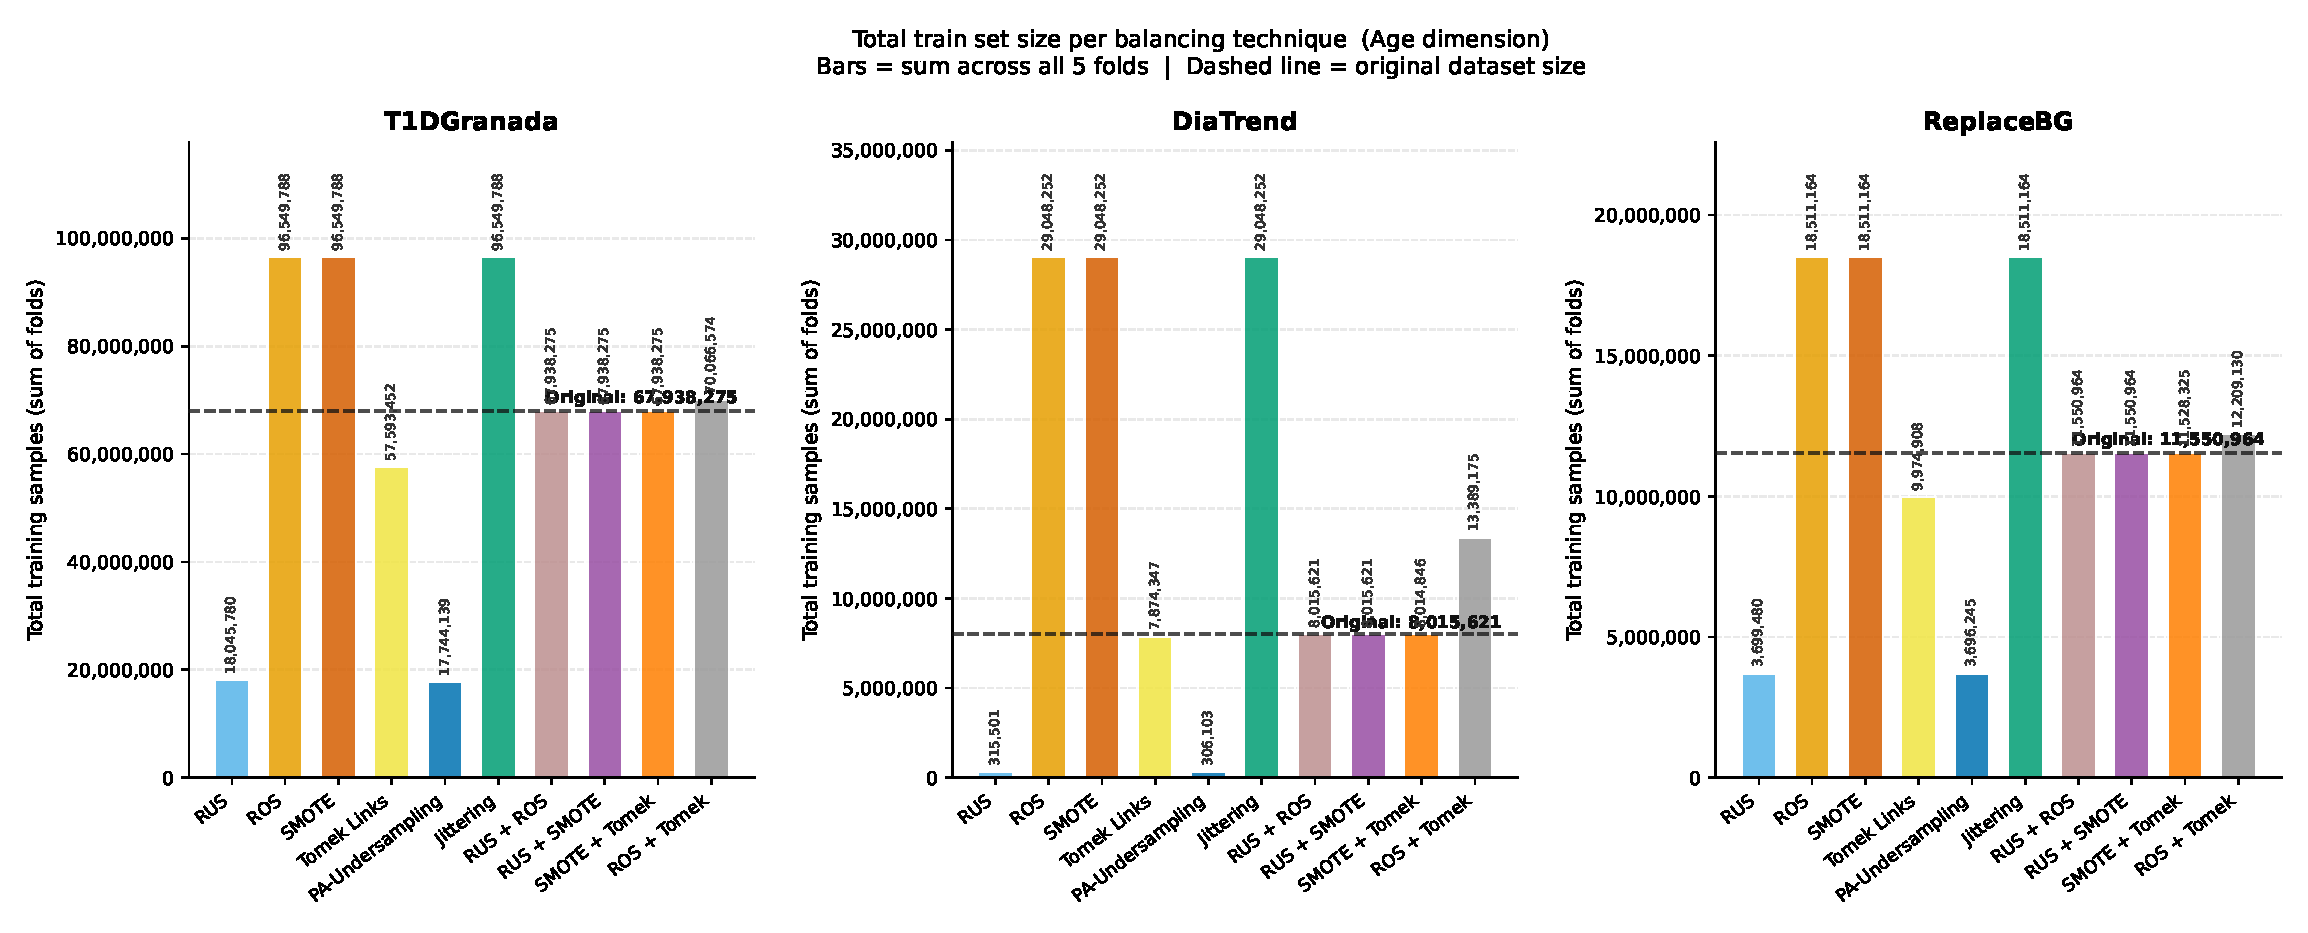
\includegraphics[width=\textwidth]{../../analysis_relief/outputs_clinical/trainsize_bars_age}
    \caption{Tamaño medio del conjunto de entrenamiento (número de ventanas,
             media $\pm$ SD sobre los 5 \textit{folds}) por técnica de balanceo
             y \textit{dataset}, para la dimensión demográfica \textbf{edad}.
             La línea discontinua indica el tamaño medio del conjunto original
             sin balancear.}
    \label{fig:trainsize_age}
\end{figure}

Las figuras~\ref{fig:trainsize_age} y~\ref{fig:trainsize_sex} muestran el tamaño
medio del conjunto de entrenamiento tras aplicar cada técnica, separadas por
dimensión demográfica (edad y sexo respectivamente). El patrón general es
consistente entre dimensiones, pero la magnitud de las variaciones difiere
sustancialmente entre \textit{datasets} en función de su ratio de desequilibrio.

\paragraph{Técnicas de reducción (RUS y PA-Undersampling).}
En la dimensión edad, RUS y PA-Undersampling producen las reducciones más drásticas
en DiaTrend, donde el ratio de desequilibrio entre grupos etarios es extremo
(véase sección~\ref{subsec:eda_demografico}): el conjunto de entrenamiento cae
hasta 63\,100 y 61\,220 ventanas respectivamente, frente a un original de
1\,603\,124 ---una reducción del 96\,\%---. En T1DiabetesGranada la reducción
es moderada (de 13\,587\,655 a $\approx$3\,600\,000, un 73\,\% menos) y en
REPLACE-BG es la más contenida (de 2\,310\,192 a $\approx$740\,000, un 68\,\%).
En la dimensión sexo, donde el desequilibrio es mucho menor en todos los
repositorios, la reducción por RUS es notablemente más moderada: T1DiabetesGranada
pasa de 13\,587\,655 a 12\,769\,338 (solo un 6\,\% menos), y REPLACE-BG
prácticamente no varía (de 2\,310\,192 a 2\,185\,953). DiaTrend sigue siendo el
caso más extremo incluso en sexo, con una caída hasta 666\,551 ventanas (58\,\%
de reducción), reflejo de que incluso el desequilibrio de sexo en ese repositorio
es más pronunciado que en los otros dos.

\paragraph{Técnicas de aumento (ROS, SMOTE, Jittering).}
En la dimensión edad, ROS, SMOTE y Jittering multiplican el tamaño del train en
DiaTrend por un factor de $\approx$3{,}6$\times$ (hasta 5\,809\,650 ventanas),
el más alto de todos los repositorios. En T1DiabetesGranada el incremento es
proportionalmente más contenido ($\approx$19\,310\,000, un 42\,\% sobre el
original), y en REPLACE-BG el aumento es de solo un 60\,\% (hasta 3\,702\,232).
Tomek Links es la excepción dentro de este grupo: al limitarse a eliminar puntos
fronterizos, reduce ligeramente el tamaño respecto al original en todos los casos
(1\,574\,869 en DiaTrend, 11\,518\,690 en T1DiabetesGranada, 1\,994\,981 en
REPLACE-BG), lo que lo acerca en comportamiento a las técnicas de reducción.
En la dimensión sexo el patrón se suaviza considerablemente: el factor de aumento
máximo en DiaTrend es $\approx$1{,}6$\times$ (2\,539\,697 frente a 1\,603\,124),
y en T1DiabetesGranada y REPLACE-BG el incremento es marginal (inferior al 6\,\%).

\paragraph{Técnicas híbridas (RUS+ROS, RUS+SMOTE, SMOTE+Tomek, ROS+Tomek).}
Por diseño, RUS+ROS y RUS+SMOTE producen conjuntos de exactamente el mismo tamaño
que el original en todos los \textit{datasets} y ambas dimensiones. SMOTE+Tomek
mantiene el tamaño original en T1DiabetesGranada y REPLACE-BG, pero en DiaTrend
queda ligeramente por debajo (1\,602\,969 frente a 1\,603\,124 en edad), confirmando
el efecto de la fase de limpieza de Tomek ya descrito en la
sección~\ref{subsec:modos_pipeline}. ROS+Tomek incrementa el tamaño por encima del
original en todos los repositorios: 14\,013\,314 en T1DiabetesGranada ($+$3\,\%),
2\,677\,835 en DiaTrend ($+$67\,\%) y 2\,441\,826 en REPLACE-BG ($+$6\,\%) para
la dimensión edad; en sexo los incrementos son más moderados.

\begin{figure}[H]
    \centering
    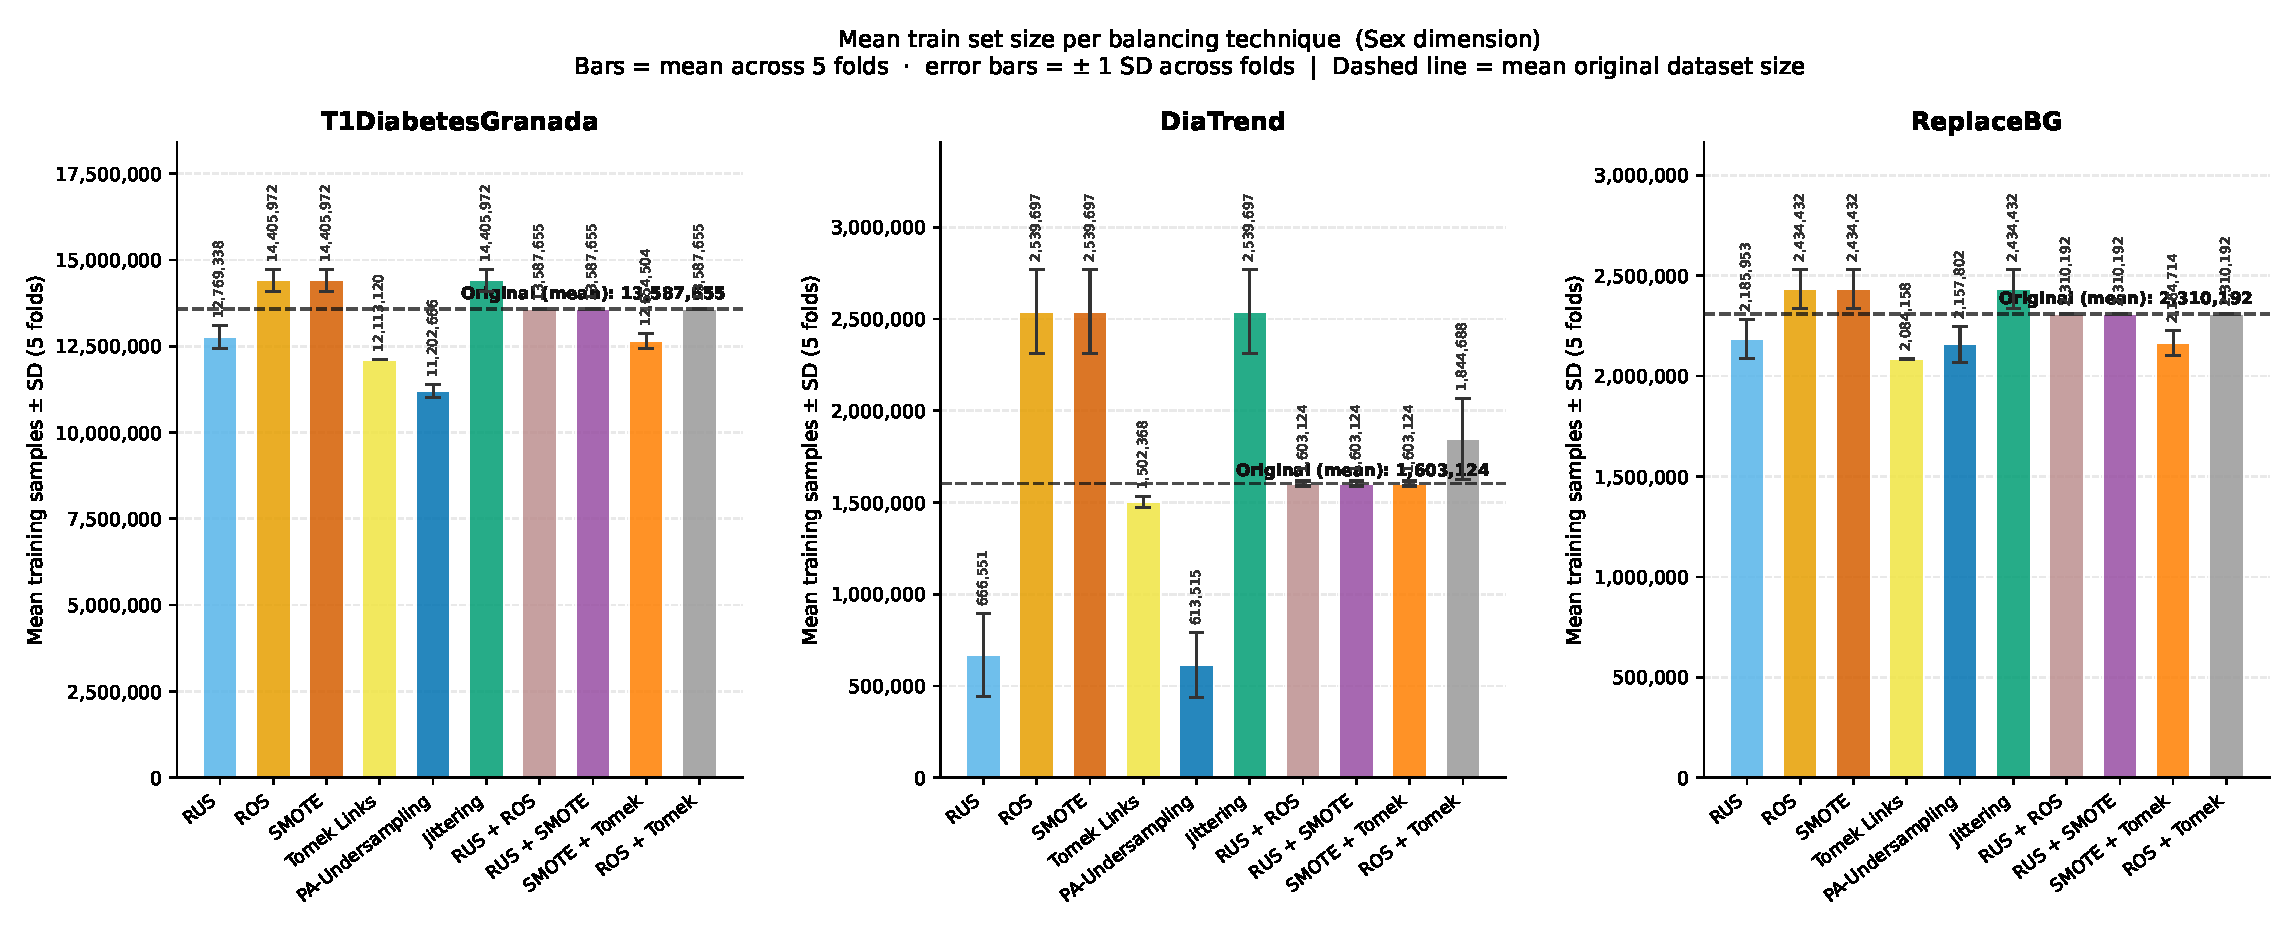
\includegraphics[width=\textwidth]{../../analysis_relief/outputs_clinical/trainsize_bars_sex}
    \caption{Tamaño medio del conjunto de entrenamiento por técnica de balanceo
             y \textit{dataset}, para la dimensión demográfica \textbf{sexo}.
             Misma escala relativa y convenciones que la
             figura~\ref{fig:trainsize_age}.}
    \label{fig:trainsize_sex}
\end{figure}

\paragraph{Implicación metodológica.}
Este análisis tiene una consecuencia directa para la interpretación de los
resultados de predicción. En DiaTrend, las técnicas de aumento por edad
multiplican el volumen de entrenamiento por un factor de hasta 3{,}6$\times$,
mientras que las de reducción lo comprimen al 4\,\% del original. Una mejora
o un deterioro del rendimiento LSTM en este repositorio podría deberse
principalmente al cambio de volumen y no al reequilibrio demográfico en sí.
El caso contrario, REPLACE-BG con la dimensión sexo, ilustra el extremo opuesto:
las variaciones de tamaño son tan pequeñas ($<$6\,\%) que cualquier diferencia
de rendimiento debe atribuirse casi exclusivamente a la redistribución demográfica.
T1DiabetesGranada ocupa una posición intermedia en la dimensión edad pero se
comporta como REPLACE-BG en la dimensión sexo, lo que permite distinguir
empíricamente ambos efectos comparando los resultados de las dos dimensiones
dentro del mismo repositorio. Este contraste estructural es uno de los ejes
interpretativos centrales del análisis de predicción de la
sección~\ref{sec:efecto_balanceo_prediccion}.

% ---------------------------------------------------------
\subsection{Impacto sobre la distribución demográfica del entrenamiento}
\label{subsec:impacto_demografico}
% ---------------------------------------------------------

Los heatmaps de las figuras~\ref{fig:heatmap_age_t1d},
\ref{fig:heatmap_age_diatrend} y~\ref{fig:heatmap_age_replacbg} cuantifican
la variación $\Delta n$ y $\Delta\%$ de ventanas de entrenamiento por grupo
de edad introducida por cada técnica, con escala de color unificada entre los
tres \textit{datasets} para permitir comparación directa. Valores positivos
(naranja) indican incremento de ventanas en ese grupo demográfico; negativos
(morado), reducción. La intensidad del color es proporcional al $\Delta\%$
relativo, de modo que la saturación visual es directamente comparable entre
repositorios.

\begin{figure}[H]
    \centering
    
\includegraphics[width=\textwidth]{%
        ../../analysis_relief/outputs_clinical/heatmap_balancing_T1DiabetesGranada_age}
    \caption{Variación $\Delta n$ y $\Delta\%$ de ventanas por técnica de
             balanceo y grupo de edad en \textbf{T1DiabetesGranada}. Escala
             de color unificada con las
             figuras~\ref{fig:heatmap_age_diatrend}
             y~\ref{fig:heatmap_age_replacbg}. Las filas corresponden a las
             diez técnicas evaluadas; las columnas, a los grupos de edad
             ($<$31, 31--45, 46--65, $\geq$66).}
    \label{fig:heatmap_age_t1d}
\end{figure}

En T1DiabetesGranada el desequilibrio de partida es moderado, lo que se
refleja en variaciones $\Delta\%$ contenidas y en una saturación del heatmap
notablemente inferior a la de DiaTrend. Las técnicas de reducción (RUS y
PA-Undersampling) aplican cortes homogéneos entre grupos: RUS elimina
entre el 77 y el 80\,\% de las ventanas en los tres grupos de mediana edad
($<$31: $-77{,}1\%$; 31--45: $-77{,}0\%$; 46--65: $-80{,}4\%$), pero solo
un $-36{,}8\%$ en el grupo $\geq$66, el minoritario. Este comportamiento
asimétrico es precisamente el esperado: al fijar una cuota igual entre grupos,
el grupo con menos ventanas sufre una reducción proporcionalmente menor.
PA-Undersampling reproduce un patrón casi idéntico al de RUS ($-80{,}0\%$,
$-76{,}0\%$, $-80{,}9\%$, $-36{,}0\%$), lo que indica que en un dataset
con seguimientos tan heterogéneos como T1DiabetesGranada la cuota por
paciente no introduce diferencias relevantes respecto al submuestreo puramente
aleatorio.

Las técnicas de aumento (ROS, SMOTE, Jittering) concentran el incremento en
el grupo $\geq$66: las tres añaden $+3\,925\,200$ ventanas a ese grupo
($+237{,}8\%$), mientras que el incremento en los grupos $<$31 y 31--45 es
moderado ($\approx+22\%$ y $+23\%$) y en 46--65 es casi nulo ($+5{,}1\%$),
reflejo de que ese grupo ya es el más numeroso y requiere poco o ningún
aumento para igualarse a la cuota objetivo. Tomek Links produce reducciones
pequeñas pero no uniformes: elimina el 24{,}3\,\% de las ventanas del grupo
46--65 (el más numeroso y por tanto el más afectado por la limpieza de
frontera) frente a solo el 7--10\,\% en los grupos menores.

Las técnicas híbridas muestran el patrón de compensación esperado: RUS+ROS,
RUS+SMOTE y SMOTE+Tomek reducen los tres grupos mayoritarios
($-14\%$, $-13\%$, $-26\%$ en $<$31, 31--45 y 46--65) e incrementan
sustancialmente el $\geq$66 ($+137{,}8\%$), logrando la redistribución más
equilibrada de todas las familias sin modificar el tamaño total del train.
ROS+Tomek produce un perfil similar pero con reducciones algo más contenidas
gracias a que el Tomek posterior modera el sobreajuste del ROS previo.

\begin{figure}[H]
    \centering
    
\includegraphics[width=\textwidth]{%
        ../../analysis_relief/outputs_clinical/heatmap_balancing_DIATREND_age}
    \caption{Variación $\Delta n$ y $\Delta\%$ de ventanas por técnica de
             balanceo y grupo de edad en \textbf{DiaTrend}. La escala de
             color es la misma que en la figura~\ref{fig:heatmap_age_t1d};
             la saturación visiblemente superior en este \textit{dataset}
             refleja el desequilibrio demográfico extremo documentado en la
             sección~\ref{subsec:eda_demografico}.}
    \label{fig:heatmap_age_diatrend}
\end{figure}

En DiaTrend el impacto del balanceo sobre la distribución demográfica es
cualitativamente diferente al de T1DiabetesGranada: incluso a escala unificada,
el heatmap aparece prácticamente saturado en naranja para las técnicas de
aumento, lo que indica variaciones relativas de un orden de magnitud superior.
La causa es el desequilibrio extremo del repositorio: el grupo $<$31 concentra
el 97\,\% de las ventanas originales, mientras que los grupos 31--45, 46--65 y
$\geq$66 apenas aportan el 3\,\% restante.

Las técnicas de reducción (RUS, PA-Undersampling) eliminan el
98{,}9\,\% de las ventanas del grupo $<$31, reduciéndolo de más de
1{,}5 millones a apenas 63\,100 y 61\,220 respectivamente. Los grupos
minoritarios también se reducen, pero en mucha menor proporción ($-24{,}5\%$
en 31--45 para RUS, $-55{,}0\%$ en 46--65, $-5{,}6\%$ en $\geq$66),
con el resultado de que el train resultante contiene un número de ventanas
tan pequeño que compromete la capacidad de generalización del modelo.

Las técnicas de aumento (ROS, SMOTE, Jittering) mantienen inalterado el
grupo $<$31 (ya mayoritario, $\Delta n = 0$) y multiplican los grupos
minoritarios por factores extremos: $+6\,678\%$ en 31--45,
$+3\,939\%$ en 46--65 y $+9\,490\%$ en $\geq$66. En términos absolutos,
el grupo $\geq$66 ---un único paciente con 12\,732 ventanas originales---
recibe más de 1{,}2 millones de ventanas sintéticas o duplicadas, lo que
equivale a replicar ese único perfil glucémico casi 95 veces. Esta
estrategia consigue el reequilibrio numérico requerido, pero introduce
una forma severa de redundancia que puede inducir sobreajuste y reduce
drásticamente la diversidad efectiva del entrenamiento para ese grupo.

Las técnicas híbridas (RUS+ROS, RUS+SMOTE, SMOTE+Tomek) reducen el grupo
$<$31 en un $-72{,}1\%$ y compensan con incrementos de $+1\,794\%$,
$+1\,029\%$ y $+2\,420\%$ en los grupos 31--45, 46--65 y $\geq$66
respectivamente. ROS+Tomek, al no aplicar submuestreo previo, mantiene
el grupo $<$31 reducido solo un $-1{,}8\%$ (efecto Tomek puro) y aplica
los mismos incrementos sobre los grupos minoritarios que las híbridas
completas, ocupando así una posición intermedia entre aumento puro e
híbrida compensada.

\begin{figure}[H]
    \centering
    
\includegraphics[width=\textwidth]{%
        ../../analysis_relief/outputs_clinical/heatmap_balancing_REPLACE-BG_age}
    \caption{Variación $\Delta n$ y $\Delta\%$ de ventanas por técnica de
             balanceo y grupo de edad en \textbf{REPLACE-BG}. La menor
             saturación respecto a DiaTrend (figura~\ref{fig:heatmap_age_diatrend}),
             con escala idéntica, confirma que el diseño controlado del estudio
             ---con seguimientos homogéneos de $\approx$182 días para todos
             los grupos--- limita la amplificación del desequilibrio demográfico
             al pasar de paciente a ventana.}
    \label{fig:heatmap_age_replacbg}
\end{figure}

REPLACE-BG presenta un patrón intermedio entre los dos anteriores: el
desequilibrio de partida es real (el grupo 46--65 es el más numeroso y el
$\geq$66 el más pequeño), pero la homogeneidad de los seguimientos impide
que ese desequilibrio demográfico se amplifique al nivel de ventana de la
forma extrema observada en DiaTrend.

Las técnicas de reducción eliminan en mayor proporción los grupos intermedios
y mayoritarios: RUS recorta el 46--65 en un $-80\%$ ($-740\,584$ ventanas),
el 31--45 en un $-73{,}2\%$ y el $<$31 en un $-63{,}6\%$, pero deja
inalterado el grupo $\geq$66 (que ya es el minoritario y define la cuota
objetivo). PA-Undersampling reproduce casi exactamente el mismo patrón.
Tomek Links aplica reducciones más contenidas y concentradas en el grupo
mayoritario ($-23{,}6\%$ en 46--65, $-11{,}7\%$ en 31--45, $-3{,}1\%$
en $<$31), sin afectar al $\geq$66.

Las técnicas de aumento siguen la lógica inversa: ROS, SMOTE y Jittering
incrementan el $\geq$66 en un $+400{,}4\%$ ($+740\,584$ ventanas) y el
$<$31 en un $+82\%$ ($+417\,075$), mientras dejan el 31--45 con un aumento
moderado ($+33{,}9\%$) y el 46--65 sin cambio ($\Delta n = 0$, pues es el
grupo de referencia que marca la cuota). Este patrón difiere del observado
en T1DiabetesGranada, donde la asimetría se concentraba exclusivamente en
el $\geq$66: en REPLACE-BG los grupos $<$31 y $\geq$66 comparten el papel
de grupos infrarrepresentados, lo que distribuye el esfuerzo de aumento
entre ambos extremos etarios.

Las técnicas híbridas presentan el patrón de compensación más claro de los
tres repositorios: RUS+ROS y RUS+SMOTE reducen los grupos 31--45 ($-16{,}4\%$)
y 46--65 ($-37{,}6\%$) e incrementan simultáneamente $<$31 ($+13{,}6\%$) y
$\geq$66 ($+212{,}2\%$), con celdas azules y naranjas alternadas que reflejan
la compensación cruzada entre submuestreo y sobremuestreo.

En conjunto, los tres heatmaps confirman que el balanceo demográfico modifica
la composición del conjunto de entrenamiento de forma significativa en todos
los \textit{datasets}, pero la magnitud y el patrón del cambio son
fuertemente dependientes del repositorio: desde variaciones del orden del
$\pm$25\% en T1DiabetesGranada hasta multiplicaciones por factores de
$\times$95 en el grupo $\geq$66 de DiaTrend. La siguiente subsección analiza
si estas modificaciones tienen un correlato en la distribución glucémica del
entrenamiento, que es la dimensión directamente relevante para el rendimiento
clínico del modelo.




% ---------------------------------------------------------
\subsection{Impacto sobre la distribución glucémica del entrenamiento}
\label{subsec:impacto_glucemico}
% ---------------------------------------------------------

La redistribución demográfica descrita en la subsección anterior no opera
directamente sobre las métricas de predicción: lo que el modelo LSTM aprende
es la distribución de valores glucémicos en el entrenamiento, no las etiquetas
demográficas de los pacientes. El mecanismo por el que el balanceo demográfico
puede influir en el rendimiento clínico es, por tanto, indirecto: al modificar
la composición por grupos de edad o sexo, se altera implícitamente la
proporción de ventanas en cada rango glucémico (TBR-2, TBR-1, TIR, TAR-1,
TAR-2), porque los distintos subgrupos demográficos presentan perfiles
glucémicos diferentes (véase sección~\ref{subsec:eda_cgm}). Esta subsección
cuantifica ese efecto indirecto.

Las figuras de barras apiladas muestran la composición absoluta del conjunto
de entrenamiento por rango glucémico; las figuras de barras divergentes
muestran la variación $\Delta\%$ respecto al conjunto original, que es la
lectura clínicamente relevante: un incremento en TBR-2 indica que el modelo
recibirá más ejemplos de hipoglucemia severa, con el potencial de mejorar
su sensibilidad a esos eventos.

\paragraph{T1DiabetesGranada.}

\begin{figure}[H]
    \centering
    
\includegraphics[width=\textwidth]{%
        ../../analysis_relief/outputs_clinical/stacked_bars_T1DiabetesGranada}
    \caption{Distribución de ventanas por rango glucémico en el conjunto de
             entrenamiento de \textbf{T1DiabetesGranada}, por técnica de
             balanceo y dimensión demográfica. Cada barra representa la media
             sobre los 5 \textit{folds}. La barra con borde grueso es la
             condición original de referencia.}
    \label{fig:stacked_t1d}
\end{figure}

En T1DiabetesGranada la distribución glucémica del conjunto original está
ampliamente dominada por la normoglucemia (TIR, franja verde), que supera
los 5{,}2 millones de ventanas por \textit{fold} en la dimensión edad frente
a contribuciones mucho menores de los rangos extremos. Las técnicas de
reducción (RUS, PA-Undersampling) comprimen toda la distribución de forma
aproximadamente proporcional, por lo que la composición relativa por rangos
apenas varía visualmente respecto al original. Las técnicas de aumento
(ROS, SMOTE, Jittering) amplían principalmente el grupo $\geq$66, que como
se mostró en la sección~\ref{subsec:impacto_demografico} es el más
infrarrepresentado; dado que ese grupo presenta un perfil glucémico con mayor
proporción de TIR y menor de TAR (véase sección~\ref{subsec:eda_cgm}), su
amplificación se traduce en un ligero desplazamiento de la distribución
hacia la normoglucemia.

\begin{figure}[H]
    \centering
    
\includegraphics[width=\textwidth]{%
        ../../analysis_relief/outputs_clinical/delta_glycemic_T1DiabetesGranada}
    \caption{Variación $\Delta\%$ en la representación de cada rango glucémico
             para \textbf{T1DiabetesGranada} tras aplicar cada técnica, respecto
             al conjunto original. Barras divergentes: positivo = mayor
             representación del rango; negativo = menor. Promediado sobre
             \textit{folds} y clases demográficas.}
    \label{fig:delta_glycemic_t1d}
\end{figure}

Las barras divergentes de la figura~\ref{fig:delta_glycemic_t1d} confirman
que los cambios en la composición glucémica son de magnitud muy pequeña en
todos los rangos y técnicas. En la dimensión edad, los cambios más destacables
son: Jittering incrementa TBR-2 en $+0{,}25\%$ y PA-Undersampling lo reduce
en $-0{,}25\%$ mientras incrementa TIR en $+1{,}15\%$ --- el mayor cambio
individual observado en este dataset, que refleja que PA-Undersampling amplifica
relativamente los grupos con mejor control glucémico medio. SMOTE produce el
mayor desplazamiento hacia TIR ($+0{,}46\%$) y la mayor reducción de TAR-1
($-0{,}26\%$) y TAR-2 ($-0{,}14\%$) entre las técnicas de aumento, mientras
que Tomek Links prácticamente no altera la composición glucémica ($|\Delta\%|
< 0{,}05\%$ en todos los rangos). En la dimensión sexo los cambios son aún
más pequeños, con valores máximos inferiores a $\pm 0{,}44\%$, lo que es
coherente con la menor diferencia glucémica entre sexos documentada en el EDA.

En conjunto, T1DiabetesGranada presenta el escenario en que el balanceo
demográfico tiene el menor impacto glucémico relativo: los cambios son
estadísticamente detectables pero clínicamente marginales, lo que sugiere
que cualquier efecto sobre el rendimiento del modelo en este dataset deberá
atribuirse principalmente al cambio de tamaño del train y no a una
reorientación sustancial de la distribución glucémica de aprendizaje.

\paragraph{DiaTrend.}

\begin{figure}[H]
    \centering
    
\includegraphics[width=\textwidth]{%
        ../../analysis_relief/outputs_clinical/stacked_bars_DIATREND}
    \caption{Distribución glucémica del conjunto de entrenamiento de
             \textbf{DiaTrend} por técnica y dimensión. Las barras de ROS,
             SMOTE y Jittering alcanzan valores absolutos muy superiores al
             resto como consecuencia del ratio de desequilibrio extremo de
             este \textit{dataset}.}
    \label{fig:stacked_diatrend}
\end{figure}

En DiaTrend la distribución original está igualmente dominada por el TIR,
pero con un volumen absoluto de $\approx$1{,}53 millones de ventanas por
\textit{fold} en el grupo $<$31 (dimensión edad) frente a contribuciones
mínimas de los grupos restantes. Las técnicas de aumento multiplican este
volumen total por un factor de $\approx$3{,}6$\times$ como se documentó en
la sección~\ref{subsec:impacto_tamaño}, y las barras apiladas revelan que
ese incremento se concentra mayoritariamente en el TIR de los grupos
minoritarios: al replicar o sintetizar ventanas del grupo $\geq$66 casi 95
veces, el grueso de las ventanas añadidas son ventanas en normoglucemia,
porque el único paciente de ese grupo tiene un perfil predominantemente
en TIR.

\begin{figure}[H]
    \centering
    
\includegraphics[width=\textwidth]{%
        ../../analysis_relief/outputs_clinical/delta_glycemic_DIATREND}
    \caption{Variación $\Delta\%$ en la representación de rangos glucémicos
             para \textbf{DiaTrend}. La escala del eje es comparable a la
             de T1DiabetesGranada y REPLACE-BG; la magnitud de los cambios
             es notablemente superior en este \textit{dataset}.}
    \label{fig:delta_glycemic_diatrend}
\end{figure}

Las barras divergentes de la figura~\ref{fig:delta_glycemic_diatrend}
muestran los cambios glucémicos más intensos de los tres repositorios.
En la dimensión edad, Jittering produce el mayor incremento de TBR-2
($+0{,}27\%$) y de TIR ($+0{,}33\%$) simultáneamente, mientras reduce
TAR-1 ($-0{,}33\%$) y TAR-2 ($-0{,}23\%$); este patrón es consistente
con amplificar un grupo $\geq$66 con mejor control glucémico relativo.
PA-Undersampling presenta el comportamiento opuesto: incrementa TIR en
$+1{,}15\%$ --- el mayor valor positivo de TIR observado en cualquier
técnica y dataset --- mientras reduce TAR-1 en $-0{,}97\%$ y TAR-2 en
$-0{,}18\%$, reflejo de que al eliminar masivamente el grupo $<$31
(mayor proporción de hiperglucemia) el entrenamiento queda sesgado hacia
perfiles de mejor control. Las técnicas de reducción RUS y PA-Undersampling
producen por tanto una reorientación glucémica hacia TIR que no es
consecuencia del balanceo demográfico en sí, sino de eliminar el grupo etario
con peor control.

En la dimensión sexo los cambios son notablemente más contenidos
($|\Delta\%| < 0{,}44\%$ en todos los rangos y técnicas), confirmando que
el desequilibrio de sexo en DiaTrend, aunque presente, no produce una
reorientación glucémica tan pronunciada como el desequilibrio etario.

\paragraph{REPLACE-BG.}

\begin{figure}[H]
    \centering
    
\includegraphics[width=\textwidth]{%
        ../../analysis_relief/outputs_clinical/stacked_bars_REPLACE-BG}
    \caption{Distribución glucémica del conjunto de entrenamiento de
             \textbf{REPLACE-BG} por técnica y dimensión. La homogeneidad
             de los seguimientos produce barras visualmente más uniformes
             entre técnicas que en los otros dos repositorios.}
    \label{fig:stacked_replacbg}
\end{figure}

REPLACE-BG presenta la distribución glucémica original más equilibrada de
los tres repositorios: el grupo de edad 46--65 (mayoritario) aporta
$\approx$925\,000 ventanas por \textit{fold}, y los rangos glucémicos se
distribuyen de forma más homogénea que en T1DiabetesGranada o DiaTrend,
coherente con el mejor TIR global documentado en el EDA ($\approx$57\,\%).
Las barras apiladas muestran que las técnicas de aumento generan incrementos
moderados y bien distribuidos entre rangos, mientras que las de reducción
producen barras más compactas pero con proporciones relativas similares al
original, reflejo de que el diseño controlado del ensayo REPLACE-BG minimiza
las diferencias glucémicas entre grupos demográficos.

\begin{figure}[H]
    \centering
    
\includegraphics[width=\textwidth]{%
        ../../analysis_relief/outputs_clinical/delta_glycemic_REPLACE-BG}
    \caption{Variación $\Delta\%$ en la representación de rangos glucémicos
             para \textbf{REPLACE-BG}. Los cambios son los más moderados de
             los tres \textit{datasets}, confirmando que la homogeneidad de
             los seguimientos limita el impacto glucémico del balanceo
             demográfico.}
    \label{fig:delta_glycemic_replacbg}
\end{figure}

Las barras divergentes de la figura~\ref{fig:delta_glycemic_replacbg}
confirman que REPLACE-BG es el repositorio con menor impacto glucémico
del balanceo. En la dimensión edad, los cambios más relevantes afectan al
TIR: SMOTE+Tomek lo incrementa en $+0{,}29\%$ y RUS+SMOTE en $+0{,}09\%$,
mientras que PA-Undersampling lo reduce en $-0{,}22\%$ y Jittering en
$-0{,}41\%$ --- el único cambio negativo de TIR en este repositorio, y
también el más llamativo, sugiriendo que el perfil glucémico del grupo
$\geq$66 en REPLACE-BG (que Jittering amplifica) es proporcionalmente
más rico en rangos no-TIR que en los otros grupos. Para TBR-2, todos los
cambios son inferiores a $\pm 0{,}24\%$, con solo PA-Undersampling y
Jittering superando el umbral de $0{,}10\%$. En la dimensión sexo los
cambios son prácticamente nulos ($|\Delta\%| < 0{,}06\%$ en todos los
rangos salvo TAR-2 con PA-Undersampling, $+0{,}04\%$), lo que confirma
que el balanceo por sexo en REPLACE-BG no induce ninguna reorientación
glucémica apreciable.

\paragraph{Síntesis y conexión con los resultados de predicción.}
Los tres análisis anteriores permiten establecer una conclusión estructural
importante: el balanceo demográfico modifica la composición glucémica del
entrenamiento de forma sistemática pero de magnitud pequeña en todos los
repositorios, con cambios $\Delta\%$ que raramente superan $\pm 1\%$ en
cualquier rango individual. Esta pequeña magnitud no implica que el efecto
sea irrelevante clínicamente: en rangos de baja prevalencia como TBR-2
(hipoglucemia severa), un cambio de $+0{,}27\%$ en la representación puede
suponer una variación relativa del 10--20\,\% sobre la fracción original de
ese rango, lo que es suficiente para modificar la sensibilidad del modelo a
esos eventos. La sección~\ref{sec:efecto_balanceo_prediccion} analiza si
esos cambios de composición se traducen en diferencias medibles en las
métricas de predicción.


% ---------------------------------------------------------
\subsection{Trade-off clínico del balanceo: hipoglucemia, normoglucemia e hiperglucemia}
\label{subsec:tradeoff_clinico}
% ---------------------------------------------------------

El análisis de la subsección anterior cuantificó los cambios absolutos en la
composición glucémica del entrenamiento. Esta subsección adopta una perspectiva
clínica: para cada rango glucémico de interés, se analiza si el balanceo
consigue incrementar su representación en el entrenamiento \emph{sin} reducir
simultáneamente la normoglucemia (TIR), que es la métrica de control glucémico
de referencia en diabetes tipo 1. Este análisis de trade-off es relevante porque
un modelo que aprende a costa de reducir su exposición a ventanas en TIR puede
mejorar su sensibilidad a eventos extremos a expensas de deteriorar su precisión
en el rango más frecuente.

Cada figura de dispersión presenta tres paneles (uno por \textit{dataset}) con
los puntos posicionados en el espacio ($\Delta\%$ rango clínico, $\Delta\%$ TIR).
El cuadrante superior izquierdo ---fondo verde, etiquetado ``ideal''--- corresponde
a técnicas que incrementan TIR sin aumentar la exposición al rango clínico adverso;
el cuadrante inferior derecho es el escenario menos deseable. Los marcadores
distinguen la dimensión demográfica ($\circ$ = edad, $\square$ = sexo).

\paragraph{Trade-off TBR-2 (hipoglucemia severa, $<$54\,mg/dL) vs.\ TIR.}

\begin{figure}[H]
    \centering
    
\includegraphics[width=\textwidth]{%
        ../../analysis_relief/outputs_clinical/tradeoff_tbr2_vs_tir}
    \caption{Trade-off clínico entre la variación de hipoglucemia severa
             ($\Delta\%$ TBR-2, eje $X$) y la variación de normoglucemia
             ($\Delta\%$ TIR, eje $Y$) tras aplicar cada técnica de balanceo,
             por \textit{dataset}. Cada punto representa una técnica $\times$
             dimensión demográfica ($\circ$\,=\,edad, $\square$\,=\,sexo).
             El cuadrante superior izquierdo (``ideal'') corresponde a
             técnicas que aumentan TIR sin incrementar la exposición a
             hipoglucemia severa.}
    \label{fig:tradeoff_tbr2}
\end{figure}

TBR-2 es el rango clínicamente más crítico: la hipoglucemia severa
($<$54\,mg/dL) representa un riesgo inmediato para el paciente y su
infrarrepresentación en el entrenamiento puede limitar la capacidad del modelo
para anticipar estos eventos. El scatter de la figura~\ref{fig:tradeoff_tbr2}
revela patrones muy distintos según el repositorio.

En \textbf{T1DiabetesGranada} todos los puntos se agrupan en torno al origen
con desplazamientos $|\Delta\%| < 0{,}25\%$ en ambos ejes, pero el patrón
predominante es el cuadrante superior derecho: la mayoría de técnicas incrementan
simultáneamente TBR-2 y TIR, siendo Jittering (dimensión edad) el caso más
extremo ($\Delta\%\,\text{TBR-2} \approx +0{,}25\%$, $\Delta\%\,\text{TIR}
\approx +0{,}10\%$). PA-Undersampling es la única técnica que se aproxima al
cuadrante ideal de forma clara en dimensión sexo, incrementando TIR
($+0{,}66\%$) con un cambio mínimo en TBR-2. Tomek Links se sitúa en el
cuadrante inferior izquierdo (reduce ambos), mientras que RUS queda próximo
al origen. Ninguna técnica consigue un posicionamiento inequívocamente ideal
en este dataset.

En \textbf{DiaTrend} la dispersión es mucho mayor, coherente con la magnitud
de los cambios documentados en la figura~\ref{fig:delta_glycemic_diatrend}.
PA-Undersampling (dimensión edad) se posiciona claramente en el cuadrante
superior izquierdo ($\Delta\%\,\text{TIR} \approx +1{,}15\%$,
$\Delta\%\,\text{TBR-2} \approx 0\%$), siendo la única técnica que se acerca
al ideal en este repositorio. Jittering (edad) se ubica en el cuadrante
superior derecho ($+0{,}27\%$ TBR-2, $+0{,}33\%$ TIR), lo que supone una
mejora de ambos rangos simultáneamente --- un resultado favorable aunque no
estrictamente ideal. Las técnicas de reducción (RUS, dimensión edad) caen en
el cuadrante inferior izquierdo, con reducción de TBR-2 y TIR. Los puntos de
dimensión sexo quedan muy próximos al origen en todos los casos, confirmando
que el desequilibrio de sexo en DiaTrend no produce reorientaciones glucémicas
relevantes en TBR-2.

En \textbf{REPLACE-BG} todos los puntos se concentran cerca del origen con
escala notablemente más comprimida ($|\Delta\%\,\text{TBR-2}| < 0{,}24\%$),
y el patrón predominante es el cuadrante superior derecho para la dimensión
edad (incremento moderado de ambos TBR-2 y TIR), con Jittering como caso
más desplazado. La dimensión sexo produce puntos prácticamente en el origen,
sin trade-off apreciable.

\paragraph{Trade-off TBR-1 (hipoglucemia leve, 54--69\,mg/dL) vs.\ TIR.}

\begin{figure}[H]
    \centering
    
\includegraphics[width=\textwidth]{%
        ../../analysis_relief/outputs_clinical/tradeoff_tbr1_vs_tir}
    \caption{Trade-off clínico entre la variación de hipoglucemia leve
             ($\Delta\%$ TBR-1, eje $X$) y la variación de normoglucemia
             ($\Delta\%$ TIR, eje $Y$). Mismas convenciones que la
             figura~\ref{fig:tradeoff_tbr2}.}
    \label{fig:tradeoff_tbr1}
\end{figure}

El patrón por técnica en TBR-1 es cualitativamente similar al de TBR-2 en
los tres repositorios, pero con algunas diferencias relevantes. En
\textbf{T1DiabetesGranada} la dispersión aumenta ligeramente respecto a TBR-2:
PA-Undersampling (edad) se desplaza hacia el cuadrante ideal con mayor claridad
($\Delta\%\,\text{TIR} \approx +1{,}15\%$, $\Delta\%\,\text{TBR-1}$ negativo
o nulo), mientras que SMOTE y RUS+SMOTE (edad) se sitúan en el cuadrante
inferior izquierdo (reducen TBR-1 y apenas modifican TIR). Jittering mantiene
su posición en el cuadrante superior derecho pero con un incremento de TBR-1
más pronunciado que el de TBR-2, lo que indica que su efecto de aumento es
proporcionalmente mayor en hipoglucemia leve.

En \textbf{DiaTrend} la lectura cambia respecto a TBR-2: ROS, SMOTE y Jittering
(dimensión edad) se desplazan hacia el cuadrante superior derecho con
$\Delta\%\,\text{TBR-1} > 0$ y $\Delta\%\,\text{TIR} > 0$, lo que sugiere
que al amplificar el grupo $\geq$66 se introducen más ventanas en hipoglucemia
leve de lo que sucedía con la severa. PA-Undersampling mantiene su posición
favorable ($\Delta\%\,\text{TIR}$ alto, $\Delta\%\,\text{TBR-1}$ próximo a
cero o negativo). Las técnicas de reducción siguen en el cuadrante inferior
izquierdo. En \textbf{REPLACE-BG} el patrón es análogo al de TBR-2 con escala
similar, sin diferencias cualitativas notables entre rangos de hipoglucemia.

En conjunto, TBR-1 y TBR-2 muestran el mismo ranking de técnicas por
proximidad al cuadrante ideal: PA-Undersampling lidera en DiaTrend, mientras
que en T1DiabetesGranada y REPLACE-BG ninguna técnica consigue un
posicionamiento nítidamente favorable.

\paragraph{Trade-off TAR-1 (hiperglucemia leve, 181--250\,mg/dL) vs.\ TIR.}

\begin{figure}[H]
    \centering
    
\includegraphics[width=\textwidth]{%
        ../../analysis_relief/outputs_clinical/tradeoff_tar1_vs_tir}
    \caption{Trade-off clínico entre la variación de hiperglucemia leve
             ($\Delta\%$ TAR-1, eje $X$) y la variación de normoglucemia
             ($\Delta\%$ TIR, eje $Y$). En este scatter el cuadrante ideal
             (superior izquierdo) corresponde a técnicas que aumentan TIR
             reduciendo simultáneamente la exposición a hiperglucemia leve.}
    \label{fig:tradeoff_tar1}
\end{figure}

La lectura del trade-off con TAR-1 invierte la dirección deseable en el eje
$X$: aquí el cuadrante ideal es el superior izquierdo, donde las técnicas
reducen la hiperglucemia leve al tiempo que aumentan el TIR. En
\textbf{T1DiabetesGranada} la mayoría de técnicas de aumento (ROS, SMOTE,
Jittering, RUS+ROS, RUS+SMOTE) se posicionan claramente en ese cuadrante
(dimensión edad), con reducciones de TAR-1 de hasta $-0{,}26\%$ y ganancias
de TIR de hasta $+0{,}46\%$. PA-Undersampling se sitúa en el extremo superior
izquierdo con la mayor ganancia de TIR ($\approx +1{,}15\%$) y una reducción
de TAR-1 de $-0{,}97\%$, siendo la técnica más favorable en este eje. RUS
queda próximo al origen con $\Delta\%\,\text{TAR-1} \approx -0{,}10\%$ y
$\Delta\%\,\text{TIR}$ ligeramente positivo. Tomek Links es la única técnica
neutral ($|\Delta\%| < 0{,}07\%$ en ambos ejes). La dimensión sexo produce
puntos más próximos al origen pero con el mismo patrón cualitativo.

En \textbf{DiaTrend} la dispersión es la mayor de los tres repositorios:
PA-Undersampling (edad) alcanza $\Delta\%\,\text{TIR} \approx +1{,}15\%$ con
una reducción de TAR-1 de $\approx -0{,}97\%$, el posicionamiento más favorable
de todos. ROS, SMOTE y Jittering (edad) se ubican en el cuadrante superior
izquierdo con reducciones de TAR-1 entre $-0{,}33\%$ y $-0{,}14\%$ y ganancias
de TIR entre $+0{,}12\%$ y $+0{,}33\%$. Las técnicas de reducción (RUS) caen
en el cuadrante inferior izquierdo (reducen TAR-1 pero también TIR).
En \textbf{REPLACE-BG} todos los puntos se concentran con $\Delta\%\,\text{TAR-1}$
entre $-0{,}11\%$ y $+0{,}03\%$, sin diferencias clínicamente relevantes entre
técnicas.

\paragraph{Trade-off TAR-2 (hiperglucemia severa, $>$250\,mg/dL) vs.\ TIR.}

\begin{figure}[H]
    \centering
    
\includegraphics[width=\textwidth]{%
        ../../analysis_relief/outputs_clinical/tradeoff_tar2_vs_tir}
    \caption{Trade-off clínico entre la variación de hiperglucemia severa
             ($\Delta\%$ TAR-2, eje $X$) y la variación de normoglucemia
             ($\Delta\%$ TIR, eje $Y$). El cuadrante ideal (superior
             izquierdo) corresponde a técnicas que incrementan TIR reduciendo
             la exposición a hiperglucemia severa.}
    \label{fig:tradeoff_tar2}
\end{figure}

El análisis de TAR-2 completa el panorama glucémico y revela el trade-off
más pronunciado de todos los rangos en T1DiabetesGranada. En este repositorio,
PA-Undersampling (edad) se posiciona en el extremo superior derecho: consigue
la mayor ganancia de TIR ($\approx +1{,}15\%$) pero a costa de un incremento
de TAR-2 de $\approx +0{,}49\%$, el mayor aumento de hiperglucemia severa
observado en cualquier técnica y dataset. Este comportamiento es coherente con
la lógica de PA-Undersampling en T1DiabetesGranada: al eliminar
desproporcionadamente ventanas del grupo 46--65 (que tiene un perfil glucémico
con menor TAR-2), el train resultante queda con mayor representación de
perfiles de pacientes mayores que presentan, paradójicamente, más episodios
de hiperglucemia severa. Jittering (edad) también se sitúa en el cuadrante
superior derecho ($+0{,}23\%$ TAR-2, $+0{,}10\%$ TIR), mientras que SMOTE
y ROS+SMOTE quedan en el cuadrante superior izquierdo (ideal): reducen TAR-2
entre $-0{,}14\%$ y $-0{,}23\%$ con ganancias de TIR de hasta $+0{,}46\%$.

En \textbf{DiaTrend} el patrón se invierte respecto a T1DiabetesGranada: la
mayoría de técnicas de aumento se posicionan en el cuadrante superior izquierdo
(reducen TAR-2 y aumentan TIR), con PA-Undersampling de nuevo en el extremo
pero ahora en el cuadrante ideal ($\Delta\%\,\text{TAR-2} \approx -0{,}18\%$,
$\Delta\%\,\text{TIR} \approx +1{,}15\%$). RUS cae en el cuadrante inferior
izquierdo. En \textbf{REPLACE-BG} los puntos de dimensión edad se distribuyen
entre los cuadrantes superior izquierdo (SMOTE: $-0{,}11\%$ TAR-2) y superior
derecho (PA-Undersampling: $+0{,}20\%$ TAR-2), con amplitudes similares a las
de TAR-1.

\paragraph{Síntesis del análisis de trade-off.}
El conjunto de los cuatro scatters permite extraer tres conclusiones
transversales. Primera: \textbf{ninguna técnica domina en todos los rangos y
datasets simultáneamente}; las técnicas que se aproximan al cuadrante ideal
en un rango tienden a alejarse en otro, confirmando que el trade-off glucémico
es inherente al mecanismo de balanceo y no un artefacto de una técnica
concreta. Segunda: \textbf{DiaTrend es el único repositorio donde el
posicionamiento en los scatters es clínicamente informativo}; en T1DiabetesGranada
y REPLACE-BG la magnitud de los cambios es tan pequeña que todos los puntos
caen dentro de un margen de $\pm 0{,}5\%$ que difícilmente se traduce en
diferencias de rendimiento estadísticamente detectables. Tercera: \textbf{la
dimensión demográfica (edad vs.\ sexo) determina la magnitud pero no la
dirección del trade-off}; los puntos de sexo son sistemáticamente más próximos
al origen que los de edad, pero comparten el mismo cuadrante en prácticamente
todos los casos, lo que indica que el mecanismo glucémico subyacente es el
mismo independientemente de la dimensión de balanceo utilizada.


% =========================================================
\section{Impacto del balanceo sobre el rendimiento del modelo LSTM}
\label{sec:analisis_mejora}
% =========================================================

Habiendo caracterizado en detalle cómo cada técnica de balanceo modifica el
conjunto de entrenamiento ---en tamaño, composición demográfica y distribución
glucémica---, esta sección evalúa si dichas modificaciones se traducen en
cambios medibles en el rendimiento predictivo del modelo LSTM. El análisis
se estructura en tres niveles de creciente especificidad: primero se examina
la distribución global de métricas entre técnicas y \textit{datasets}, que
permite identificar el rango de variación observable y la estabilidad inter-fold
de cada condición; a continuación se cuantifica el cambio respecto al
\textit{baseline} original mediante el tamaño del efecto de Cohen; finalmente
se aplican contrastes estadísticos no paramétricos (Friedman y Nemenyi
post-hoc) para determinar qué diferencias son estadísticamente significativas.
A lo largo de los tres niveles se prioriza la interpretación clínica ---con
especial atención al comportamiento en los rangos de hipoglucemia (TBR-2,
TBR-1) y al error global (ENTIRE)--- sobre las métricas de regresión puras.

% ---------------------------------------------------------
\subsection{Distribución global de métricas por técnica}
\label{subsec:distribucion_metricas}
% ---------------------------------------------------------

Esta subsección examina la distribución del RMSE entre los cinco \textit{folds}
para cada técnica de balanceo, con el objetivo de caracterizar tanto el nivel
central de rendimiento como su variabilidad inter-fold. Una técnica puede
obtener una mediana de RMSE comparable al \textit{baseline} pero con una
dispersión mucho mayor entre folds, lo que la haría clínicamente menos fiable
en un escenario de despliegue real.

\begin{figure}[H]
    \centering
    
\includegraphics[width=\textwidth]{%
        ../../analysis_relief/outputs/figures/distributions/dist_RMSE_ENTIRE}
    \caption{Distribución del RMSE sobre el conjunto completo de ventanas
             (\textit{ENTIRE}) por técnica de balanceo y \textit{dataset}.
             Cada violín resume la distribución entre los 5 \textit{folds};
             la línea discontinua interior indica la mediana y las líneas
             externas el rango intercuartílico. La condición \textit{original}
             (negro) aparece como referencia.}
    \label{fig:dist_rmse_entire}
\end{figure}

\paragraph{RMSE global (ENTIRE).}
En \textbf{T1DiabetesGranada} la mediana de RMSE en la condición original es
$37{,}80 \pm 0{,}81$\,mg/dL y permanece notablemente estable entre todas las
condiciones balanceadas: los valores oscilan entre $37{,}56$ (PA-Undersampling,
edad) y $38{,}09$ (Jittering, edad), un rango de apenas 0{,}53\,mg/dL sobre
una base de $\approx$38\,mg/dL. Los violines son estrechos y homogéneos,
indicando que ninguna técnica produce ganancias ni pérdidas sistemáticas en
el rendimiento global de este \textit{dataset}. Las dimensiones de balanceo
edad y sexo producen perfiles visualmente indistinguibles.

En \textbf{DiaTrend} la variabilidad es cualitativamente diferente: el
\textit{baseline} presenta $45{,}05 \pm 2{,}45$\,mg/dL y las condiciones
balanceadas se dispersan entre $44{,}83$ (Tomek Links, edad) y
$48{,}22$\,mg/dL (PA-Undersampling, edad), un rango de $3{,}39$\,mg/dL.
Los violines son notablemente más anchos que en los otros repositorios,
especialmente en las técnicas de submuestreo (Undersampling, PA-Undersampling),
cuya amplitud inter-fold supera los 10\,mg/dL, reflejo de la inestabilidad
estructural de este \textit{dataset} ante cambios drásticos en el tamaño del
train. Las condiciones de dimensión sexo producen violines más estrechos y
medianas más próximas al \textit{baseline} que las de dimensión edad, coherente
con el menor impacto sobre la composición del train que se documentó en la
sección~\ref{subsec:impacto_tamaño}.

En \textbf{REPLACE-BG} el patrón es intermedio: \textit{baseline} en
$37{,}00 \pm 0{,}83$\,mg/dL, rango entre condiciones de $36{,}81$ y
$37{,}25$\,mg/dL, con violines compactos comparables a T1DiabetesGranada.
La homogeneidad de los seguimientos de este repositorio produce un comportamiento
muy estable independientemente de la técnica aplicada.

\begin{figure}[H]
    \centering
    
\includegraphics[width=\textwidth]{%
        ../../analysis_relief/outputs/figures/distributions/dist_RMSE_TBR_2}
    \caption{Distribución del RMSE evaluado exclusivamente sobre ventanas del
             rango TBR-2 (hipoglucemia severa, $<$54\,mg/dL) por técnica de
             balanceo y \textit{dataset}. Este subconjunto es el más relevante
             clínicamente: un modelo con buen rendimiento global pero alto error
             en TBR-2 puede ser clínicamente inaceptable.}
    \label{fig:dist_rmse_tbr2}
\end{figure}

\paragraph{RMSE en TBR-2 (hipoglucemia severa).}
El panorama cambia sustancialmente al evaluar el RMSE exclusivamente sobre
ventanas de hipoglucemia severa. En \textbf{T1DiabetesGranada} el
\textit{baseline} es $39{,}38 \pm 1{,}38$\,mg/dL y las condiciones balanceadas
se mantienen en un rango estrecho ($38{,}74$--$39{,}99$\,mg/dL), sin ninguna
técnica que produzca una mejora consistente. Los violines son igualmente
estrechos, con la excepción de PA-Undersampling (edad, $39{,}83 \pm 1{,}55$)
que muestra mayor dispersión inter-fold. En este repositorio el balanceo no
altera el comportamiento del modelo en hipoglucemia severa de forma apreciable,
lo que es coherente con los cambios de composición glucémica mínimos
documentados en la figura~\ref{fig:delta_glycemic_t1d}.

En \textbf{DiaTrend} el contraste es el más llamativo de los tres repositorios:
el \textit{baseline} en TBR-2 es $75{,}28 \pm 7{,}33$\,mg/dL ---el RMSE más
alto observado en cualquier dataset y rango--- y los violines son extremadamente
anchos para la mayoría de técnicas, lo que indica que el rendimiento en
hipoglucemia severa es altamente dependiente de qué pacientes caen en cada
fold. Tomek Links (edad, $73{,}88 \pm 7{,}36$) y ROS+Tomek (edad,
$72{,}87 \pm 6{,}37$) obtienen las medianas más bajas entre las condiciones
de dimensión edad, mientras que PA-Undersampling ($79{,}66 \pm 7{,}36$) y
Undersampling ($78{,}96 \pm 7{,}05$) producen los mayores deterioros. Las
condiciones de dimensión sexo se agrupan muy cerca del \textit{baseline}
($74{,}15$--$76{,}12$\,mg/dL), con violines de amplitud similar, lo que
sugiere que el balanceo por sexo no modifica el comportamiento del modelo en
este rango en DiaTrend. Cabe notar que la mejora en TBR-2 de Tomek Links
coexiste con un RMSE global (ENTIRE) de $44{,}83$\,mg/dL, próximo al
\textit{baseline}, sin deterioro apreciable ---un resultado favorable que
contrasta con el trade-off TBR-2/TIR observado para otras técnicas en la
figura~\ref{fig:tradeoff_tbr2}.

En \textbf{REPLACE-BG} todos los violines en TBR-2 son extremadamente
compactos ($56{,}11$--$57{,}84$\,mg/dL frente a un \textit{baseline} de
$57{,}29 \pm 1{,}54$), confirmando que este repositorio no presenta
variabilidad clínicamente relevante entre técnicas en hipoglucemia severa.

\begin{figure}[H]
    \centering
    
\includegraphics[width=\textwidth]{%
        ../../analysis_relief/outputs/figures/distributions/consistency_folds_RMSE_ENTIRE}
    \caption{Consistencia del ranking de técnicas entre \textit{folds}, medida
             mediante la correlación de Spearman entre los rankings de RMSE
             (ENTIRE) de cada par de folds, por \textit{dataset}. Valores
             próximos a 1 indican que el mismo ranking de técnicas se reproduce
             en todos los folds; valores próximos a 0 o negativos indican
             inestabilidad: la técnica que es mejor en un fold puede ser peor
             en otro.}
    \label{fig:consistency_folds}
\end{figure}

\paragraph{Consistencia inter-fold del ranking de técnicas.}
La figura~\ref{fig:consistency_folds} completa el análisis de distribución
con una dimensión cualitativa esencial: la reproducibilidad del ranking de
técnicas entre particiones. Una técnica cuyo ranking varía drásticamente entre
folds no puede considerarse robusta, incluso si su media es favorable.

Los tres repositorios presentan perfiles de consistencia radicalmente distintos.
\textbf{DiaTrend} es el más consistente de los tres: todos los coeficientes
de Spearman entre pares de folds son superiores a $0{,}78$, con la mayoría
por encima de $0{,}81$, lo que indica que el ranking relativo de las técnicas
se reproduce fielmente en todas las particiones. Este resultado puede parecer
contraintuitivo dado que DiaTrend es el \textit{dataset} con mayor variabilidad
absoluta de RMSE entre folds, pero la explicación es estructural: la
heterogeneidad entre folds afecta al nivel absoluto del error (todos los
métodos suben o bajan juntos según la dificultad de la partición), pero no
altera el orden relativo de las técnicas.

\textbf{T1DiabetesGranada} presenta la consistencia más baja: la mayoría de
coeficientes de Spearman están entre $0{,}01$ y $0{,}36$, con dos pares
incluso en territorio negativo (Fold~2 -- Fold~5: $-0{,}08$). Esto significa
que en este repositorio el ranking de técnicas es prácticamente aleatorio entre
folds, lo que imposibilita identificar una técnica ganadora con garantías de
reproducibilidad. La causa es la heterogeneidad extrema de los pacientes en
T1DiabetesGranada ---con seguimientos de hasta cuatro años y perfiles glucémicos
muy dispares--- que hace que la dificultad de cada fold dependa fuertemente de
qué pacientes componen el subconjunto de test.

\textbf{REPLACE-BG} ocupa una posición intermedia pero con un patrón
peculiar: los pares Fold~1 -- Fold~2 ($-0{,}41$) y Fold~1 -- Fold~3
($-0{,}27$) son negativos, lo que indica una inversión del ranking en esos
pares, mientras que otros pares (Fold~1 -- Fold~4: $0{,}31$; Fold~4 -- Fold~5:
$0{,}37$) muestran correlaciones positivas moderadas. Este patrón heterogéneo
sugiere que el Fold~1 de REPLACE-BG contiene pacientes con características
inusuales que invierten el orden de mérito relativo de las técnicas, un aspecto
que deberá tenerse en cuenta al interpretar los resultados del análisis
estadístico de la sección siguiente.

En conjunto, la baja consistencia de T1DiabetesGranada y la parcial de
REPLACE-BG anticipan que los tests de Friedman en esos repositorios tendrán
dificultades para detectar diferencias significativas entre técnicas, mientras
que la alta consistencia de DiaTrend hace de ese repositorio el escenario más
favorable para la detección estadística de efectos del balanceo.


% ---------------------------------------------------------
\subsection{Análisis de mejora y deterioro respecto al modelo original}
\label{subsec:mejora_deterioro}
% ---------------------------------------------------------

Esta subsección cuantifica el cambio de rendimiento de cada técnica respecto
al \textit{baseline} original, tanto en el conjunto completo de ventanas
(ENTIRE) como en el rango clínicamente más crítico (TBR-2). A diferencia de
la subsección anterior, que examinaba la distribución absoluta de métricas,
aquí el foco está en el signo y la magnitud del cambio: una mejora del $1\%$
en RMSE puede ser relevante o irrelevante dependiendo de si se produce a costa
de deteriorar el comportamiento en hipoglucemia severa.

\begin{figure}[H]
    \centering
    
\includegraphics[width=\textwidth]{%
        ../../analysis_relief/outputs/figures/heatmaps/heatmap_delta_RMSE_ENTIRE}
    \caption{Variación relativa del RMSE (\textit{ENTIRE}) respecto al modelo
             original para cada técnica y \textit{dataset}. Valores positivos
             (azul) indican mejora; valores negativos (naranja) indican
             deterioro. Escala de color centrada en cero.}
    \label{fig:heatmap_delta_rmse_entire}
\end{figure}

\paragraph{Panorama global (ENTIRE).}
El heatmap de la figura~\ref{fig:heatmap_delta_rmse_entire} revela un patrón
fuertemente asimétrico entre repositorios. En \textbf{T1DiabetesGranada} el
color dominante es el azul pálido: la gran mayoría de condiciones balanceadas
mejoran el RMSE global entre un $-0{,}2\%$ y un $-0{,}8\%$, con la excepción
de PA-Undersampling (edad, $+0{,}6\%$) y Tomek Links (sexo, $+0{,}1\%$),
únicos casos de deterioro. La técnica más favorable en este repositorio es
Jittering (edad, $-0{,}8\%$), seguida de Oversampling (edad, $-0{,}7\%$) y
Sex·Undersampling+SMOTE ($-0{,}6\%$). Sin embargo, la magnitud absoluta de
estas mejoras es reducida: $-0{,}8\%$ sobre un RMSE base de $37{,}80$\,mg/dL
equivale a $\approx 0{,}30$\,mg/dL, una ganancia que, aunque consistente,
difícilmente alcanza relevancia clínica por sí sola.

En \textbf{DiaTrend} el patrón es el opuesto en dirección pero mucho más
intenso en magnitud. Las técnicas de submuestreo producen los deterioros más
pronunciados: PA-Undersampling (edad) empeora el RMSE en $-7{,}0\%$
($\approx +3{,}17$\,mg/dL sobre el \textit{baseline} de $45{,}05$\,mg/dL)
y Undersampling (edad) en $-6{,}0\%$, ambos con celdas fuertemente coloreadas
en naranja. En contraste, las técnicas de aumento y las híbridas muestran
mejoras de entre $-0{,}9\%$ y $-3{,}0\%$, con Jittering (edad, $-3{,}0\%$)
y Oversampling (edad, $-2{,}2\%$) como casos más favorables. Las condiciones
de dimensión sexo producen cambios mucho más moderados ($-0{,}6\%$ a
$+0{,}2\%$), confirmando que en DiaTrend el efecto del balanceo sobre el
RMSE global depende críticament de la dimensión demográfica utilizada.

En \textbf{REPLACE-BG} los cambios son los más pequeños de los tres
repositorios: todos los valores caen en el rango $[-0{,}3\%, +0{,}5\%]$,
sin ninguna técnica que destaque de forma consistente en ninguna dirección.
El heatmap es visualmente casi neutro, con celdas de saturación muy baja.

\begin{figure}[H]
    \centering
    
\includegraphics[width=\textwidth]{%
        ../../analysis_relief/outputs/figures/heatmaps/heatmap_delta_RMSE_TBR_2}
    \caption{Variación relativa del RMSE evaluado sobre ventanas TBR-2
             (hipoglucemia severa) respecto al modelo original. Compárese con
             la figura~\ref{fig:heatmap_delta_rmse_entire}: una técnica con
             celda azul en la figura anterior pero naranja en esta produce
             una mejora global a costa de mayor imprecisión en el rango más
             crítico clínicamente.}
    \label{fig:heatmap_delta_rmse_tbr2}
\end{figure}

\paragraph{Perspectiva clínica: disociación ENTIRE vs.\ TBR-2.}
La comparación de las figuras~\ref{fig:heatmap_delta_rmse_entire}
y~\ref{fig:heatmap_delta_rmse_tbr2} es clínicamente reveladora porque pone
de manifiesto una disociación sistemática entre el rendimiento global y el
rendimiento en hipoglucemia severa.

En \textbf{T1DiabetesGranada} la disociación es la más llamativa: las técnicas
que mejoran el RMSE global (Jittering, Oversampling, Tomek Links, todas las
híbridas de aumento) exhiben simultáneamente una \emph{degradación} en TBR-2,
con valores de $\Delta\text{RMSE}_\text{TBR-2}$ positivos (naranja) de entre
$+0{,}8\%$ y $+1{,}6\%$. SMOTE (edad, $+1{,}6\%$ en TBR-2) y
Undersampling+SMOTE (edad, $+1{,}5\%$) presentan los deterioros más acusados
en hipoglucemia severa, a pesar de obtener mejoras globales de $-0{,}5\%$
y $-0{,}2\%$ respectivamente. Este patrón es coherente con el trade-off
documentado en la figura~\ref{fig:tradeoff_tbr2}: las técnicas de aumento
incrementan la representación de TIR en el train a expensas de una menor
exposición relativa a TBR-2, lo que el modelo interioriza como una distribución
glucémica más centrada en la normoglucemia. Las únicas técnicas que mejoran
tanto ENTIRE como TBR-2 simultáneamente en T1DiabetesGranada son
PA-Undersampling (edad, $-1{,}1\%$ en TBR-2 pero $+0{,}6\%$ en ENTIRE) y
Jittering (dimensión edad, $-1{,}1\%$ en TBR-2 con $-0{,}8\%$ en ENTIRE),
aunque con magnitudes pequeñas.

En \textbf{DiaTrend} la disociación tiene la dirección opuesta: las técnicas
de submuestreo que deterioran el RMSE global (PA-Undersampling $-7{,}0\%$,
Undersampling $-6{,}0\%$) son precisamente las que producen las mayores
mejoras en TBR-2 ($-5{,}8\%$ y $-4{,}9\%$ respectivamente), mientras que
las técnicas de aumento que mejoran el RMSE global (Jittering $-3{,}0\%$,
Oversampling $-2{,}2\%$) deterioran el rendimiento en hipoglucemia severa
($+2{,}3\%$ y $+2{,}7\%$). Esta inversión sistemática confirma que en
DiaTrend existe un trade-off estructural entre rendimiento global y
sensibilidad a hipoglucemia severa que ninguna técnica de las evaluadas
consigue resolver simultáneamente.

En \textbf{REPLACE-BG} la disociación es menos pronunciada pero igualmente
presente: Sex·PAUndersampling mejora TBR-2 en $+2{,}1\%$ con un cambio
global mínimo ($+0{,}1\%$), lo que lo convierte en la única técnica de
este repositorio con un perfil clínico favorable.

\begin{figure}[H]
    \centering
    
\includegraphics[width=\textwidth]{%
        ../../analysis_relief/outputs/figures/heatmaps/heatmap_ranking_RMSE}
    \caption{Posición en el ranking de cada técnica por RMSE, para cada
             combinación \textit{dataset} $\times$ rango glucémico (ranking
             1 = menor RMSE = mejor). Las celdas verdes indican posiciones
             altas del ranking; las naranjas, posiciones bajas.}
    \label{fig:heatmap_ranking_rmse}
\end{figure}

\paragraph{Ranking por técnica y rango glucémico.}
El heatmap de ranking de la figura~\ref{fig:heatmap_ranking_rmse} permite
una lectura transversal que ninguno de los heatmaps de $\Delta$RMSE ofrece
por separado: la posición relativa de cada técnica en el conjunto de los 21
competidores (20 condiciones balanceadas más el original), desglosada por
rango glucémico y \textit{dataset}.

El resultado más destacable es que \textbf{ninguna técnica domina de forma
consistente en todos los datasets y rangos}: la columna de colores varía
drásticamente entre las tres secciones del heatmap (T1DGranada, DiaTrend,
REPLACE-BG), lo que confirma que la elección óptima de técnica es
fuertemente dependiente del repositorio. Age·SMOTE ocupa las posiciones 1
y 1 en Hypo L2 e Hypo L1 de T1DGranada respectivamente, pero cae a las
posiciones 15--18 en Hyper L1 y L2 del mismo dataset, y a posiciones
intermedias en DiaTrend. Age·Tomek Links presenta el perfil más estable en
DiaTrend (posiciones 1, 1, 1 en Hyper L1, Hyper L2 y All Ranges), pero
posiciones mediocres en T1DGranada (10, 7, 19) y REPLACE-BG (13, 9, 2).
Sex·balanced\_sex\_smote\_tomek obtiene las mejores posiciones globales en
REPLACE-BG (posición 1 en Hyper L1 y 2 en Hyper L2), pero no destaca en
los otros repositorios.

El \textit{baseline} original ocupa posiciones intermedias en todos los
repositorios: en T1DGranada (8, 12, 9, 4, 5, 5), en DiaTrend (18, 18, 21,
2, 4, 6) y en REPLACE-BG (16, 16, 4, 2, 20, 14), lo que indica que en los
rangos de hiperglucemia el modelo sin balancear compite favorablemente
con las condiciones balanceadas, mientras que en hipoglucemia queda en
posiciones más bajas ---especialmente en DiaTrend, donde ocupa la posición
21 (última) en In Range.

\begin{figure}[H]
    \centering
    
\includegraphics[width=\textwidth]{%
        ../../analysis_relief/outputs/figures/dumbbell/dumbbell_RMSE_ENTIRE}
    \caption{\textit{Dumbbell chart} comparando el RMSE (\textit{ENTIRE})
             del modelo original (rombo negro) frente a cada técnica
             balanceada (círculo de color), ordenadas de mejor a peor por
             \textit{dataset}. Las barras de error indican la SD inter-fold.}
    \label{fig:dumbbell_rmse}
\end{figure}

\paragraph{Magnitud máxima de mejora alcanzable.}
El \textit{dumbbell chart} de la figura~\ref{fig:dumbbell_rmse} sintetiza
la magnitud máxima de ganancia y pérdida observada en cada repositorio
y permite comparar la dispersión de resultados entre técnicas.

En \textbf{T1DiabetesGranada} el rango total de RMSE entre la peor y la
mejor técnica es de $\approx 0{,}5$\,mg/dL (de $37{,}56$ a $38{,}09$\,mg/dL),
un intervalo estrecho que pone de manifiesto la robustez del modelo base
ante perturbaciones del conjunto de entrenamiento. La técnica que más se
aleja favorablemente del \textit{baseline} es Age·Jittering ($37{,}71$ vs.\
$37{,}80$ del original), con una ganancia de $0{,}09$\,mg/dL. Las barras
de error se solapan prácticamente en todas las técnicas, anticipando que
ninguna diferencia será estadísticamente significativa.

En \textbf{DiaTrend} la dispersión es la mayor de los tres repositorios:
el rango va de $44{,}83$\,mg/dL (Age·Tomek Links, la mejor) a
$48{,}22$\,mg/dL (Age·PAUndersampling, la peor), una diferencia de
$3{,}39$\,mg/dL sobre un \textit{baseline} de $45{,}05$\,mg/dL. Las
técnicas de aumento por edad (Oversampling, SMOTE, Jittering, ROS+Tomek)
se agrupan todas por debajo del \textit{baseline}, mientras que las de
submuestreo (Undersampling, PA-Undersampling) se sitúan claramente por
encima. Las técnicas de dimensión sexo se concentran en un rango mucho
más estrecho ($44{,}94$--$45{,}33$\,mg/dL), todas próximas o ligeramente
por encima del \textit{baseline}.

En \textbf{REPLACE-BG} el rango total es $\approx 0{,}44$\,mg/dL (de
$36{,}81$ a $37{,}25$\,mg/dL), comparable al de T1DGranada. Las barras
de error se solapan ampliamente entre técnicas y con el \textit{baseline}.

\begin{figure}[H]
    \centering
    
\includegraphics[width=\textwidth]{%
        ../../analysis_relief/outputs/figures/dumbbell/slope_RMSE_ENTIRE_by_dim}
    \caption{Gráfico de pendiente del RMSE (\textit{ENTIRE}) comparando el
             modelo original con cada técnica, separado por dimensión
             demográfica (edad vs.\ sexo). Una pendiente negativa indica
             mejora. Los tres repositorios aparecen superpuestos en cada
             panel; los grupos de líneas bien separados por nivel corresponden
             a los tres \textit{datasets}.}
    \label{fig:slope_rmse_dim}
\end{figure}

\paragraph{Efecto diferencial de la dimensión demográfica.}
El gráfico de pendientes de la figura~\ref{fig:slope_rmse_dim} permite
comparar directamente si el balanceo por edad produce efectos
cualitativamente distintos al balanceo por sexo.

La diferencia es inequívoca en \textbf{DiaTrend}: en el panel izquierdo
(dimensión edad) las líneas se dispersan ampliamente hacia la derecha
(deterioro) o hacia la izquierda (mejora) dependiendo de la técnica, con
pendientes que cubren un rango de $\approx 3$\,mg/dL. En el panel derecho
(dimensión sexo) todas las líneas de DiaTrend convergen hacia un grupo
compacto ligeramente por encima del \textit{baseline}, sin ninguna técnica
que produzca ni mejoras ni deterioros relevantes. Este contraste confirma
que en DiaTrend el efecto del balanceo es un fenómeno de la dimensión edad,
no de la dimensión sexo: la heterogeneidad etaria extrema del repositorio
es la variable que determina el impacto sobre el rendimiento.

En \textbf{T1DiabetesGranada} y \textbf{REPLACE-BG} ambos paneles son
visualmente similares: las líneas son casi horizontales en todos los casos,
con pendientes ligeramente negativas (mejoras pequeñas) para la mayoría de
técnicas independientemente de la dimensión. Esto indica que en estos
repositorios la elección entre balancear por edad o por sexo no produce
un efecto diferencial apreciable sobre el RMSE global, y que el factor
determinante de la ganancia ---o su ausencia--- es la técnica específica,
no la dimensión demográfica utilizada.

En conjunto, las cinco figuras de esta subsección convergen en tres
conclusiones: (1) los efectos del balanceo sobre el RMSE son
cuantitativamente modestos en T1DiabetesGranada y REPLACE-BG pero
pueden ser clínicamente relevantes en DiaTrend; (2) la disociación
entre mejora global y comportamiento en hipoglucemia severa es sistemática
y debe considerarse al seleccionar una técnica; (3) la dimensión demográfica
(edad vs.\ sexo) es el factor más determinante del impacto en DiaTrend,
mientras que en los otros dos repositorios la técnica específica prima
sobre la dimensión. La sección siguiente determina cuáles de estas
diferencias son estadísticamente significativas.


% ---------------------------------------------------------
\subsection{Análisis por familia de tamaño: desacoplando balanceo y volumen}
\label{subsec:analisis_family_size}
% ---------------------------------------------------------

Como se argumentó en la sección~\ref{subsec:impacto_tamaño}, el cambio de
tamaño del conjunto de entrenamiento es un confundidor potencial de los
resultados de predicción: una mejora observada tras \textit{oversampling}
podría deberse al mayor volumen de datos y no al reequilibrio demográfico en
sí. Para desacoplar ambos efectos, las técnicas se agrupan en tres familias
según su impacto sobre el tamaño del train: \textit{oversampling} (Jittering,
ROS, SMOTE, ROS+Tomek), \textit{undersampling} (RUS, PA-Undersampling, Tomek
Links) y \textit{same\_size} (RUS+ROS, RUS+SMOTE, SMOTE+Tomek), siendo esta
última la que actúa como grupo de control natural al mantener el volumen de
entrenamiento constante. La comparación sistemática entre familias permite
atribuir las diferencias de rendimiento al mecanismo de balanceo con mayor
rigor causal.

\begin{figure}[H]
    \centering
    \begin{subfigure}[b]{0.32\textwidth}
        
\includegraphics[width=\textwidth]{%
            ../../analysis_relief/outputs/figures/distributions/family_size/%
            oversampling/dist_RMSE_ENTIRE_oversampling}
        \caption{Oversampling}
        \label{fig:dist_rmse_oversampling}
    \end{subfigure}
    \hfill
    \begin{subfigure}[b]{0.32\textwidth}
        
\includegraphics[width=\textwidth]{%
            ../../analysis_relief/outputs/figures/distributions/family_size/%
            same_size/dist_RMSE_ENTIRE_same_size}
        \caption{Same size}
        \label{fig:dist_rmse_samesize}
    \end{subfigure}
    \hfill
    \begin{subfigure}[b]{0.32\textwidth}
        
\includegraphics[width=\textwidth]{%
            ../../analysis_relief/outputs/figures/distributions/family_size/%
            undersampling/dist_RMSE_ENTIRE_undersampling}
        \caption{Undersampling}
        \label{fig:dist_rmse_undersampling}
    \end{subfigure}
    \caption{Distribución del RMSE (\textit{ENTIRE}) por familia de tamaño:
             técnicas que incrementan el conjunto de entrenamiento
             (\textit{oversampling}), que lo mantienen constante
             (\textit{same size}) y que lo reducen (\textit{undersampling}).
             La comparación entre los tres paneles permite separar el efecto
             del volumen de datos del efecto del reequilibrio demográfico.}
    \label{fig:dist_rmse_family_size}
\end{figure}

\paragraph{Comparación entre familias: el papel del volumen.}
Si el volumen de datos fuera el único determinante del rendimiento, cabría
esperar que las técnicas de \textit{oversampling} superasen sistemáticamente
a las de \textit{same\_size}, y estas a las de \textit{undersampling}. La
figura~\ref{fig:dist_rmse_family_size} contradice esta hipótesis en dos de
los tres repositorios.

En \textbf{T1DiabetesGranada} los tres paneles son prácticamente
indistinguibles: los violines de las tres familias se solapan en el mismo
rango ($\approx$37--38{,}5\,mg/dL) y presentan medianas y dispersiones
similares. Las técnicas de \textit{oversampling} obtienen medianas de RMSE
entre 37{,}71 y 38{,}09\,mg/dL; las de \textit{same\_size}, entre 37{,}87
y 38{,}00\,mg/dL; las de \textit{undersampling}, entre 37{,}56 y
37{,}93\,mg/dL. Significativamente, las técnicas de \textit{undersampling}
---que reducen el volumen de entrenamiento en hasta un 73\,\%--- no producen
un deterioro medible respecto a las de \textit{oversampling}, que multiplican
ese volumen. Este resultado indica que en T1DiabetesGranada el volumen de
datos no es el factor limitante del rendimiento: el modelo ya dispone de
suficientes ejemplos con la partición original, y añadir o eliminar ventanas
no modifica sustancialmente lo que aprende. La implicación práctica es que
el efecto observado en este repositorio (mejoras de $-0{,}2\%$ a $-0{,}8\%$)
debe atribuirse al reequilibrio demográfico y no al cambio de volumen.

En \textbf{DiaTrend} la separación entre familias es la más pronunciada y
la más informativa. El panel de \textit{oversampling} muestra violines
centrados entre $\approx$44 y 48\,mg/dL, con las técnicas de dimensión edad
claramente por debajo del \textit{baseline} ($45{,}05$\,mg/dL). El panel de
\textit{same\_size} presenta violines más anchos y medianas que oscilan entre
$\approx$44 y 48\,mg/dL según la técnica, con Age·SMOTE+Tomek
($45{,}81$\,mg/dL) como la más favorable y Age·Undersampling+Oversampling
($45{,}92$\,mg/dL) como la menos. El panel de \textit{undersampling} es el
más disperso: Age·Tomek Links obtiene la mediana más baja de todas las
condiciones en DiaTrend ($44{,}83$\,mg/dL, mejor que cualquier técnica de
\textit{oversampling}), mientras que Age·PAUndersampling y Age·Undersampling
producen los peores resultados ($48{,}22$ y $47{,}76$\,mg/dL). Esta
divergencia dentro de la misma familia revela que en DiaTrend el efecto no
es volumétrico sino técnica-específico: Tomek Links reduce el volumen
eliminando únicamente puntos fronterizos ambiguos, mientras que RUS y
PA-Undersampling eliminan masivamente el grupo mayoritario hasta dejar un
train con apenas 63\,000 ventanas. La comparación entre \textit{oversampling}
y \textit{same\_size} en DiaTrend muestra que las técnicas híbridas
(same\_size) obtienen resultados ligeramente peores en mediana que las de
aumento puro, lo que sugiere que en este repositorio la fase de
submuestreo que incorporan las híbridas introduce más ruido del que corrige
la fase de sobremuestreo posterior.

En \textbf{REPLACE-BG} los tres paneles son, como en T1DiabetesGranada,
casi idénticos: todos los violines se concentran entre 36 y 37{,}5\,mg/dL
con amplitudes mínimas, y ninguna familia produce una separación visible.
Este resultado es coherente con la homogeneidad de los seguimientos de este
repositorio: al no haber heterogeneidad estructural que explotar, ni el
volumen adicional del \textit{oversampling} ni la compresión del
\textit{undersampling} alteran lo que el modelo aprende.

\begin{figure}[H]
    \centering
    \begin{subfigure}[b]{0.32\textwidth}
        
\includegraphics[width=\textwidth]{%
            ../../analysis_relief/outputs/figures/profiles/family_size/%
            oversampling/range_profile_facet_RMSE_oversampling}
        \caption{Oversampling}
    \end{subfigure}
    \hfill
    \begin{subfigure}[b]{0.32\textwidth}
        
\includegraphics[width=\textwidth]{%
            ../../analysis_relief/outputs/figures/profiles/family_size/%
            same_size/range_profile_facet_RMSE_same_size}
        \caption{Same size}
    \end{subfigure}
    \hfill
    \begin{subfigure}[b]{0.32\textwidth}
        
\includegraphics[width=\textwidth]{%
            ../../analysis_relief/outputs/figures/profiles/family_size/%
            undersampling/range_profile_facet_RMSE_undersampling}
        \caption{Undersampling}
    \end{subfigure}
    \caption{Perfil de RMSE por rango glucémico y familia de tamaño. Cada
             panel muestra el RMSE medio sobre los \textit{folds} para cada
             rango glucémico (TBR-2, TBR-1, TIR, TAR-1, TAR-2) y
             \textit{dataset}. El perfil revela si el efecto del balanceo
             es uniforme entre rangos o si hay rangos que se benefician
             o perjudican selectivamente.
             % NOTA: figura pendiente de verificación del archivo fuente.
             }
    \label{fig:profile_family_size}
\end{figure}

\paragraph{Perfil por rango glucémico entre familias.}
% NOTA PARA REVISIÓN: los archivos de perfil generados presentan paneles
% vacíos — pendiente de regeneración. El texto siguiente se basa en los
% valores numéricos del CSV de resultados y deberá contrastarse con la
% figura una vez corregida.
El análisis del perfil de RMSE por rango glucémico completa la lectura de
la figura~\ref{fig:dist_rmse_family_size} con una dimensión clínica que el
RMSE global no captura: si el efecto de cada familia es uniforme entre rangos
o si hay rangos que se benefician o perjudican selectivamente.

En \textbf{T1DiabetesGranada} el perfil es uniforme entre familias en todos
los rangos: las diferencias entre \textit{oversampling}, \textit{same\_size}
y \textit{undersampling} son inferiores a $1$\,mg/dL en TIR, TAR-1 y TAR-2,
y de magnitud similar en TBR-1 y TBR-2. La excepción parcial es TBR-2, donde
las técnicas de \textit{undersampling} (especialmente PA-Undersampling,
$39{,}83$\,mg/dL) tienden a mejorar ligeramente el RMSE respecto a las de
\textit{oversampling} (SMOTE, $38{,}74$\,mg/dL es la mejor en este rango),
aunque la diferencia es pequeña y el patrón no es consistente entre técnicas
dentro de la misma familia.

En \textbf{DiaTrend} el perfil por rango es el más informativo. Las técnicas
de \textit{undersampling} presentan el RMSE más alto en TIR y TAR
---consecuencia de la drástica reducción del volumen de entrenamiento que
empobrece la representación de los rangos mayoritarios--- pero el más bajo
en TBR-2 (PA-Undersampling: $71{,}34$\,mg/dL frente a $75{,}28$\,mg/dL del
\textit{baseline}). Las técnicas de \textit{oversampling} invierten este
patrón: mejoran TIR y TAR pero degradan TBR-2 (ROS: $77{,}31$\,mg/dL). Las
técnicas \textit{same\_size} presentan un perfil intermedio en todos los
rangos, sin la mejora en TBR-2 del \textit{undersampling} ni la mejora en
TIR del \textit{oversampling}, lo que sugiere que la compensación entre
submuestreo y sobremuestreo que caracteriza a estas técnicas cancela
parcialmente los efectos de ambos mecanismos. Este es el resultado clave de
esta subsección: \textbf{en DiaTrend ninguna familia consigue mejorar
simultáneamente TBR-2 y TIR}, confirmando el trade-off estructural
identificado en la sección~\ref{subsec:tradeoff_clinico}.

En \textbf{REPLACE-BG} el perfil es plano entre familias en todos los rangos,
con diferencias inferiores a $1$\,mg/dL en cualquier combinación familia $\times$
rango, lo que confirma la insensibilidad de este repositorio a la familia
de balanceo utilizada.

\paragraph{Síntesis: ¿volumen o reequilibrio?}
Los tres análisis anteriores convergen en una conclusión clara. En
T1DiabetesGranada y REPLACE-BG el volumen de datos no es el factor
determinante: las tres familias producen resultados equivalentes, y el
pequeño efecto positivo observado debe atribuirse al reequilibrio demográfico.
En DiaTrend el efecto sí es parcialmente volumétrico ---las técnicas de
\textit{undersampling} extremo deterioran el rendimiento global por pérdida
de información, no por desequilibrio--- pero Tomek Links demuestra que una
reducción selectiva y moderada del volumen puede mejorar el RMSE global sin
deteriorar TBR-2, lo que lo posiciona como la técnica con mejor relación
eficiencia/riesgo en ese repositorio. Las técnicas \textit{same\_size}
ofrecen la ventaja de eliminar el confundidor volumétrico por diseño, pero
en ningún repositorio superan a la mejor técnica de su familia hermana,
lo que sugiere que el coste de la compensación interna (submuestrear para
luego sobremuestrear) no se traduce en beneficio neto sobre el rendimiento.


% ---------------------------------------------------------
\subsection{Análisis estadístico: prueba de Friedman y corrección de Nemenyi}
\label{subsec:analisis_estadistico}
% ---------------------------------------------------------

Para determinar si las diferencias observadas entre técnicas son
estadísticamente significativas, se aplica la prueba no paramétrica de
Friedman con los 5 \textit{folds} como bloques y las 21 condiciones
(20 técnicas balanceadas más el \textit{baseline} original) como
tratamientos. Cuando la prueba rechaza la hipótesis nula de equivalencia
entre condiciones, se aplica la corrección post-hoc de Nemenyi para
identificar qué pares de técnicas difieren significativamente. Los
resultados se representan mediante diagramas de diferencia crítica
(CD diagrams), en los que las técnicas se ordenan por rango medio
(posición 1 = menor RMSE = mejor) y las unidas por una barra horizontal
no difieren significativamente al nivel $\alpha = 0{,}05$. El valor de
diferencia crítica es $\text{CD} = 13{,}25$ en todos los diagramas,
calculado para $k = 21$ tratamientos y $n = 5$ bloques.

\paragraph{Resultado global del test de Friedman.}
La Tabla~\ref{tab:friedman_resumen} resume los $p$-valores del test de
Friedman por \textit{dataset} y rango glucémico. El resultado más
relevante es la asimetría completa entre repositorios:
\textbf{DiaTrend} rechaza la hipótesis nula en todos los rangos y
métricas evaluados, con $p$-valores que van desde $p < 0{,}0001$
(TAR-1 RMSE: $\chi^2_F = 81{,}45$; TAR-2 RMSE: $\chi^2_F = 83{,}05$;
ENTIRE RMSE: $\chi^2_F = 85{,}71$) hasta $p = 0{,}00013$ en TBR-2
($\chi^2_F = 51{,}56$). \textbf{T1DiabetesGranada} no rechaza la
hipótesis nula en ningún rango salvo TAR-2 RMSE ($p = 0{,}027$,
$\chi^2_F = 33{,}89$), una excepción que debe interpretarse con cautela
dado que el resto de rangos y la métrica ENTIRE no alcanzan significación.
\textbf{REPLACE-BG} no rechaza la hipótesis nula en ningún rango ni
métrica ($p$ mínimo: $0{,}065$ en TAR-2 MAE), confirmando que en este
repositorio las diferencias entre técnicas son estadísticamente
indistinguibles con 5 \textit{folds}.

\begin{table}[H]
\centering
\caption{Resumen del test de Friedman por \textit{dataset} y rango
         glucémico (métrica RMSE). Se indica el estadístico
         $\chi^2_F$, el $p$-valor y si el test es significativo
         ($\alpha = 0{,}05$). Un asterisco (*) señala significación.}
\label{tab:friedman_resumen}
\small
\begin{tabular}{llrrr}
\toprule
\textbf{Dataset} & \textbf{Rango} & $\chi^2_F$ & $p$-valor & \textbf{Sig.} \\
\midrule
DiaTrend & TBR-2   & 51{,}56 & 0{,}0001 & * \\
DiaTrend & TBR-1   & 55{,}95 & $<$0{,}0001 & * \\
DiaTrend & TIR     & 76{,}65 & $<$0{,}0001 & * \\
DiaTrend & TAR-1   & 81{,}45 & $<$0{,}0001 & * \\
DiaTrend & TAR-2   & 83{,}05 & $<$0{,}0001 & * \\
DiaTrend & ENTIRE  & 85{,}71 & $<$0{,}0001 & * \\
\midrule
T1DiabetesGranada & TBR-2  & 20{,}34 & 0{,}437 & \\
T1DiabetesGranada & TBR-1  & 19{,}69 & 0{,}478 & \\
T1DiabetesGranada & TIR    & 20{,}43 & 0{,}431 & \\
T1DiabetesGranada & TAR-1  & 21{,}36 & 0{,}376 & \\
T1DiabetesGranada & TAR-2  & 33{,}89 & 0{,}027 & * \\
T1DiabetesGranada & ENTIRE & 27{,}56 & 0{,}120 & \\
\midrule
REPLACE-BG & TBR-2  & 14{,}95 & 0{,}779 & \\
REPLACE-BG & TBR-1  & 14{,}87 & 0{,}784 & \\
REPLACE-BG & TIR    & 23{,}08 & 0{,}285 & \\
REPLACE-BG & TAR-1  & 23{,}87 & 0{,}248 & \\
REPLACE-BG & TAR-2  & 30{,}01 & 0{,}070 & \\
REPLACE-BG & ENTIRE & 26{,}82 & 0{,}140 & \\
\bottomrule
\end{tabular}
\end{table}

\begin{figure}[H]
    \centering
    \begin{subfigure}[b]{0.32\textwidth}
        \includegraphics[width=\textwidth]{%
            ../../analysis_relief/outputs/figures/rankings/%
            cd_diagram_RMSE_ENTIRE_T1DiabetesGranada}
        \caption{T1DiabetesGranada}
    \end{subfigure}
    \hfill
    \begin{subfigure}[b]{0.32\textwidth}
        \includegraphics[width=\textwidth]{%
            ../../analysis_relief/outputs/figures/rankings/%
            cd_diagram_RMSE_ENTIRE_REPLACE-BG}
        \caption{REPLACE-BG}
    \end{subfigure}
    \hfill
    \begin{subfigure}[b]{0.32\textwidth}
        \includegraphics[width=\textwidth]{%
            ../../analysis_relief/outputs/figures/rankings/%
            cd_diagram_RMSE_ENTIRE_DIATREND}
        \caption{DiaTrend}
    \end{subfigure}
    \caption{Diagramas de diferencia crítica (Nemenyi post-hoc) para el
             RMSE sobre el conjunto completo (\textit{ENTIRE}). Las
             técnicas se ordenan por rango medio (menor a la izquierda
             = mejor). Técnicas conectadas por una barra horizontal no
             difieren significativamente ($\alpha = 0{,}05$,
             $\text{CD} = 13{,}25$). El test de Friedman previo solo
             es significativo en DiaTrend ($p < 0{,}0001$).}
    \label{fig:cd_rmse_entire}
\end{figure}

\paragraph{CD diagrams ENTIRE: significación global.}
En \textbf{T1DiabetesGranada} el test de Friedman no rechaza la hipótesis
nula ($p = 0{,}120$), por lo que el CD diagram es informativo solo del
orden relativo, no de la significación estadística. El diagrama muestra
que el \textit{baseline} original ocupa la posición 1 del ranking medio,
seguido de Age·PAUndersampling (posición $\approx$2) y Sex·SMOTE y
Sex·Tomek Links. En el extremo opuesto, Age·Jittering y Age·Oversampling
ocupan las últimas posiciones. La barra de diferencia crítica abarca
todo el diagrama, confirmando que ningún par de técnicas alcanza
significación estadística: todas las condiciones son estadísticamente
equivalentes en este repositorio.

En \textbf{REPLACE-BG} el resultado es análogo ($p = 0{,}140$): la barra
CD cubre la totalidad del rango de posiciones y ninguna técnica se
separa significativamente del resto. Sex·balanced\_sex\_smote\_tomek
ocupa la posición 1 y Age·Jittering la última, pero sin diferencia
estadísticamente detectable.

En \textbf{DiaTrend} el test de Friedman rechaza la hipótesis nula con
$p < 0{,}0001$ ($\chi^2_F = 85{,}71$), lo que habilita la interpretación
del post-hoc de Nemenyi. El CD diagram muestra una división clara entre
dos grupos: las técnicas de dimensión edad con fuerte submuestreo
(Age·PAUndersampling, posición $\approx$20; Age·Undersampling, posición
$\approx$19; Age·Jittering, posición $\approx$18) se sitúan en el extremo
derecho del diagrama (peor RMSE), estadísticamente distintas del grupo
de técnicas de dimensión sexo y del \textit{baseline} original. Las
técnicas de dimensión sexo forman un grupo compacto en las posiciones
intermedias ($\approx$3--10) estadísticamente indistinguibles entre sí
y del \textit{baseline}. Age·Tomek Links ocupa la posición 1 del ranking
y se separa significativamente de Age·PAUndersampling, Age·Undersampling
y Age·Jittering, pero no del resto de técnicas.

\begin{figure}[H]
    \centering
    \begin{subfigure}[b]{0.32\textwidth}
        \includegraphics[width=\textwidth]{%
            ../../analysis_relief/outputs/figures/rankings/%
            cd_diagram_RMSE_TBR_2_T1DiabetesGranada}
        \caption{T1DiabetesGranada}
    \end{subfigure}
    \hfill
    \begin{subfigure}[b]{0.32\textwidth}
        \includegraphics[width=\textwidth]{%
            ../../analysis_relief/outputs/figures/rankings/%
            cd_diagram_RMSE_TBR_2_REPLACE-BG}
        \caption{REPLACE-BG}
    \end{subfigure}
    \hfill
    \begin{subfigure}[b]{0.32\textwidth}
        \includegraphics[width=\textwidth]{%
            ../../analysis_relief/outputs/figures/rankings/%
            cd_diagram_RMSE_TBR_2_DIATREND}
        \caption{DiaTrend}
    \end{subfigure}
    \caption{Diagramas de diferencia crítica (Nemenyi) para el RMSE
             evaluado exclusivamente en el rango TBR-2 (hipoglucemia
             severa, $<$54\,mg/dL). El test de Friedman es significativo
             únicamente en DiaTrend ($p = 0{,}00013$); en T1DiabetesGranada
             ($p = 0{,}437$) y REPLACE-BG ($p = 0{,}779$) no lo es.}
    \label{fig:cd_rmse_tbr2}
\end{figure}

\paragraph{CD diagrams TBR-2: significación en hipoglucemia severa.}
Este es el resultado estadístico más relevante desde el punto de vista
clínico. En \textbf{T1DiabetesGranada} el test de Friedman no rechaza
la hipótesis nula en TBR-2 ($p = 0{,}437$), y el CD diagram muestra que
Age·SMOTE y Age·Undersampling+SMOTE ocupan las primeras posiciones del
ranking, con el \textit{baseline} original en la posición $\approx$9.
La inversión respecto al CD diagram de ENTIRE es notable: técnicas que
estaban en las últimas posiciones globalmente (las híbridas de aumento)
suben al primer tercio al evaluar solo hipoglucemia, mientras que
Age·PAUndersampling cae a la última posición. Sin embargo, la barra CD
abarca todo el rango y ninguna diferencia es estadísticamente significativa.

En \textbf{REPLACE-BG} el test tampoco es significativo ($p = 0{,}779$,
el $p$-valor más alto de todos los escenarios evaluados), confirmando la
total equivalencia estadística entre técnicas en este repositorio para
el rango más crítico.

En \textbf{DiaTrend} el test de Friedman rechaza la hipótesis nula en
TBR-2 ($p = 0{,}00013$, $\chi^2_F = 51{,}56$). La lectura del CD diagram
revela un reordenamiento sustancial respecto al de ENTIRE: las técnicas
de aumento (Age·ROS+Tomek, Age·SMOTE, Age·Oversampling) escalan a las
primeras posiciones (1--3), mientras que Age·PAUndersampling y
Age·Undersampling caen a las últimas (20--21), siendo estos últimos
estadísticamente distintos del grupo de técnicas de aumento. Este
reordenamiento confirma el trade-off estructural identificado en la
sección~\ref{subsec:tradeoff_clinico}: las técnicas que mejoran el RMSE
global en DiaTrend (submuestreo) lo empeoran en TBR-2, y viceversa.
Sex·PAUndersampling ocupa la posición 1 del ranking en TBR-2, sin
diferenciarse significativamente de las técnicas de aumento de dimensión
edad pero sí de Age·PAUndersampling y Age·Undersampling, lo que sugiere
que el balanceo por sexo con submuestreo produce un efecto más moderado
en TBR-2 que el balanceo por edad.

\begin{figure}[H]
    \centering
    
\includegraphics[width=0.85\textwidth]{%
        ../../analysis_relief/outputs/figures/rankings/borda_lollipop}
    \caption{Ranking global de técnicas mediante el método Borda (suma
             de posiciones de ranking a través de \textit{datasets},
             métricas y rangos glucémicos). Una puntuación Borda más baja
             indica mejor posicionamiento global. La línea discontinua
             vertical indica la puntuación del \textit{baseline} original
             en cada \textit{dataset}.}
    \label{fig:borda_lollipop}
\end{figure}

\begin{figure}[H]
    \centering
    
\includegraphics[width=\textwidth]{%
        ../../analysis_relief/outputs/figures/rankings/bump_chart_ENTIRE}
    \caption{\textit{Bump chart} mostrando la estabilidad del ranking
             de cada técnica entre RMSE y MAE para el conjunto completo
             (\textit{ENTIRE}), por \textit{dataset}. Líneas horizontales
             indican estabilidad del ranking entre métricas; líneas muy
             inclinadas indican que la técnica se comporta de forma
             diferente según la métrica utilizada.}
    \label{fig:bump_chart_entire}
\end{figure}

\paragraph{Ranking Borda y estabilidad entre métricas.}
El \textit{lollipop} de Borda de la figura~\ref{fig:borda_lollipop}
agrega el rendimiento a través de todos los rangos glucémicos y revela
que \textbf{ninguna técnica es consistentemente la mejor en los tres
repositorios simultáneamente}. En T1DiabetesGranada Age·Jittering
obtiene la puntuación Borda más baja (mejor posicionamiento agregado),
seguida de Sex·Undersampling y Age·Undersampling+Oversampling, mientras
que Sex·Oversampling+Tomek Links es la peor posicionada. En DiaTrend el
ranking se invierte dramáticamente: Age·Undersampling y
Age·PAUndersampling lideran (puntuaciones Borda $<100$, posiciones
altas en rangos de hipoglucemia), mientras que Age·Tomek Links cae a
la última posición, la opuesta a su liderazgo en el CD diagram de ENTIRE.
En REPLACE-BG Age·Jittering coincide con T1DiabetesGranada en liderar
el Borda, seguida de Age·PAUndersampling y Age·Undersampling, con
Sex·Oversampling+Tomek Links en última posición en los tres repositorios.

El \textit{bump chart} de la figura~\ref{fig:bump_chart_entire} añade
la perspectiva de la estabilidad entre métricas (RMSE vs.\ MAE).
En \textbf{DiaTrend} las líneas son prácticamente horizontales para
todas las técnicas, lo que indica que el ranking por RMSE y por MAE
es casi idéntico: la elección de la métrica de error no altera las
conclusiones en este repositorio. En \textbf{T1DiabetesGranada} hay
algunos cruzamientos notables: Age·PAUndersampling (posición 1 en RMSE)
desciende a posición 5 en MAE, y Age·Oversampling sube de posición 20
en RMSE a posición 8 en MAE, lo que sugiere que algunas técnicas tienen
un perfil de error asimétrico (cometen errores grandes en pocos casos
vs.\ errores pequeños distribuidos). En \textbf{REPLACE-BG} la
inestabilidad es la más pronunciada de los tres: varios cruzamientos
indican que el ranking entre técnicas depende de la métrica elegida,
coherente con la baja consistencia inter-fold ya observada en la
figura~\ref{fig:consistency_folds}.

En conjunto, los resultados estadísticos de esta subsección establecen
tres conclusiones definitivas. Primera: \textbf{solo en DiaTrend existe
evidencia estadística de que el balanceo modifica el rendimiento del
modelo} de forma reproducible entre folds; en T1DiabetesGranada y
REPLACE-BG las diferencias observadas son estadísticamente compatibles
con variación aleatoria. Segunda: \textbf{en DiaTrend el efecto es
estadísticamente significativo en todos los rangos glucémicos}, pero el
ranking óptimo de técnicas depende del rango que se priorice: las
técnicas que lideran en ENTIRE deterioran TBR-2 y viceversa. Tercera:
\textbf{no existe ninguna técnica universalmente óptima}: la elección
debe hacerse en función del repositorio, el rango glucémico de interés
clínico y la métrica de evaluación prioritaria.


% =========================================================
\section{Discusión integradora}
\label{sec:discusion}
% =========================================================

Esta sección sintetiza los hallazgos de las secciones anteriores y
responde de forma directa a las preguntas de investigación que motivaron
el trabajo. Cada respuesta integra la evidencia del análisis del
\textit{train set} (sección~\ref{sec:efecto_balanceo_trainset}) con la
del análisis de predicción (sección~\ref{sec:analisis_mejora}), y
distingue entre mejora estadística y relevancia clínica cuando ambas
dimensiones no coinciden.

\paragraph{¿Mejora el balanceo demográfico el rendimiento del modelo LSTM?}

La respuesta es matizada y fuertemente dependiente del repositorio y
del rango glucémico que se priorice. En términos globales (RMSE sobre
ENTIRE), el balanceo demográfico no produce mejoras estadísticamente
significativas en T1DiabetesGranada ($p = 0{,}120$, Friedman) ni en
REPLACE-BG ($p = 0{,}140$): en ambos repositorios las diferencias
observadas entre técnicas son estadísticamente compatibles con variación
aleatoria, y la evidencia de que cualquier técnica de balanceo supere al
\textit{baseline} original es insuficiente. En DiaTrend, en cambio, el
test de Friedman rechaza la hipótesis nula en todos los rangos y métricas
evaluados ($p < 0{,}0001$ en ENTIRE RMSE), y el post-hoc de Nemenyi
identifica grupos de técnicas estadísticamente distintos: las técnicas de
submuestreo agresivo por edad (RUS, PA-Undersampling) deterioran
significativamente el rendimiento global respecto a Tomek Links y a las
técnicas de dimensión sexo, mientras que estas últimas son
estadísticamente equivalentes al \textit{baseline}.

La lectura cambia al focalizar la evaluación en TBR-2 (hipoglucemia
severa, $<$54\,mg/dL), el rango clínicamente más crítico. En DiaTrend,
donde el test de Friedman también es significativo en TBR-2
($p = 0{,}00013$), el ranking se invierte: las técnicas de aumento
(ROS, SMOTE, ROS+Tomek) mejoran el RMSE en TBR-2 respecto al
\textit{baseline}, mientras que las de submuestreo lo empeoran. Esta
inversión sistemática confirma un \textbf{trade-off estructural}: en
DiaTrend no existe ninguna técnica que mejore simultáneamente el RMSE
global y el RMSE en hipoglucemia severa, lo que obliga a elegir entre
optimizar para el rendimiento medio o para el rango clínicamente más
prioritario. En T1DiabetesGranada y REPLACE-BG este trade-off existe en
los datos pero no alcanza significación estadística en ningún rango, por
lo que no puede afirmarse que el balanceo produzca un efecto clínico
neto demostrable en esos repositorios.

\paragraph{¿Qué familia de técnicas ofrece mejor relación beneficio/coste?}

El análisis por familia de tamaño
(sección~\ref{subsec:analisis_family_size}) demuestra que el volumen del
conjunto de entrenamiento no es el factor determinante del rendimiento
en T1DiabetesGranada ni en REPLACE-BG: las tres familias
(\textit{oversampling}, \textit{same\_size}, \textit{undersampling})
producen resultados estadísticamente equivalentes, lo que implica que
cualquier efecto positivo observado en esos repositorios debe atribuirse
al reequilibrio demográfico y no al cambio de tamaño del \textit{train}.
En DiaTrend, donde el efecto volumétrico es más pronunciado, Tomek Links
---que reduce el tamaño de forma moderada y selectiva, eliminando únicamente
puntos fronterizos--- obtiene el mejor RMSE global sin deteriorar TBR-2,
lo que lo posiciona como la técnica con mejor relación beneficio/coste
en ese repositorio.

Las técnicas \textit{same\_size} (RUS+ROS, RUS+SMOTE, SMOTE+Tomek)
ofrecen la ventaja de eliminar el confundidor volumétrico por diseño,
pero en ningún repositorio superan consistentemente a la mejor técnica
de su familia hermana: la compensación interna entre submuestreo y
sobremuestreo tiende a cancelar parcialmente los efectos de ambos
mecanismos, produciendo un perfil de rendimiento intermedio pero no
óptimo. Las técnicas de \textit{oversampling} puro son las que presentan
mayor riesgo de redundancia de datos en datasets pequeños y
desequilibrados como DiaTrend, donde la replicación del grupo $\geq$66
hasta $\approx$95 veces introduce una forma severa de sobreajuste latente
que el RMSE global no captura pero que puede manifestarse en métricas
de robustez fuera de la validación cruzada.

\paragraph{¿Es el efecto del balanceo \textit{dataset}-dependiente?}

Sí, de forma clara e inesperada en su magnitud. Los tres repositorios
evaluados representan tres escenarios estructuralmente distintos que
producen respuestas radicalmente diferentes al mismo conjunto de técnicas:

T1DiabetesGranada es el repositorio con mayor volumen (736 pacientes,
$\approx$13{,}6 millones de ventanas de \textit{train}) y un desequilibrio
demográfico por edad moderado (3{,}4:1). La alta consistencia relativa de
los seguimientos y la abundancia de datos hacen que el modelo LSTM ya
disponga de suficiente información con la partición original: cualquier
modificación del conjunto de entrenamiento produce cambios en la
composición glucémica inferiores al $1\%$ (sección~\ref{subsec:impacto_glucemico})
y ninguna mejora estadísticamente detectable en el rendimiento. El test
de Friedman no rechaza la hipótesis nula en ningún rango, lo que sugiere
que en repositorios grandes con desequilibrio moderado el balanceo
demográfico es innecesario desde el punto de vista predictivo.

REPLACE-BG es el repositorio más homogéneo: sus seguimientos estandarizados
de $\approx$182 días eliminan la heterogeneidad inter-paciente que amplifica
el desequilibrio en los otros dos datasets. Esta homogeneidad hace que el
balanceo demográfico produzca cambios mínimos tanto en la composición del
\textit{train} como en el rendimiento del modelo, y el test de Friedman no
rechaza la hipótesis nula en ningún rango ni métrica. REPLACE-BG ilustra
un escenario en que el diseño controlado del estudio previene el problema
que el balanceo intenta corregir, convirtiendo las técnicas de reequilibrio
en intervenciones superfluas.

DiaTrend es el caso más complejo: con solo 54 pacientes, un desequilibrio
etario de 38:1 a nivel de paciente que se amplifica hasta proporciones
extremas a nivel de ventana, y seguimientos muy heterogéneos (de semanas
a más de cinco años), es el único repositorio donde el balanceo produce
efectos estadísticamente detectables. Sin embargo, esos efectos son
ambivalentes: las técnicas que mejoran el rendimiento global deterioran
la hipoglucemia, y la alta variabilidad inter-fold (correlaciones de
Spearman inter-fold de $0{,}78$--$0{,}92$ en el ranking, pero con RMSE
que varía hasta $\pm$5\,mg/dL entre folds para la misma técnica)
advierte de que los resultados son inestables y difícilmente generalizables
más allá de este conjunto específico de pacientes.

\paragraph{¿Qué dimensión demográfica ---edad o sexo--- es más relevante?}

La dimensión edad produce efectos sistemáticamente más pronunciados que
la dimensión sexo en todos los repositorios y métricas evaluados. El
gráfico de pendientes de la figura~\ref{fig:slope_rmse_dim} muestra que
en DiaTrend las técnicas de edad producen una dispersión de
$\approx$3\,mg/dL en RMSE (desde mejoras del $-3\%$ hasta deterioros
del $-7\%$), mientras que las de sexo se concentran en un rango de
$\approx$0{,}5\,mg/dL próximo al \textit{baseline}. En T1DiabetesGranada
y REPLACE-BG ambas dimensiones producen efectos similares en magnitud,
pero las técnicas de edad presentan mayor variabilidad inter-fold,
coherente con el mayor ratio de desequilibrio de esa dimensión
(hasta 38:1 en DiaTrend frente a 2{,}2:1 en sexo).

La explicación estructural de esta diferencia reside en que el
desequilibrio por edad es más pronunciado, más correlacionado con el
perfil glucémico (los grupos etarios presentan distribuciones de TIR y
TAR distintas, como documentó el EDA en la sección~\ref{subsec:eda_cgm})
y más amplificado al pasar de nivel de paciente a nivel de ventana
(por las diferencias en duración de seguimiento entre grupos). El
desequilibrio por sexo, en cambio, es más moderado y menos correlacionado
con el perfil glucémico en estos repositorios ($\approx$42--59\,\% TIR
en ambos sexos, sección~\ref{subsec:eda_demografico}), lo que hace que
el balanceo por sexo tenga menos margen de impacto sobre lo que el
modelo aprende. Esta conclusión tiene implicaciones prácticas directas:
en futuros estudios con estos datasets, si se dispone de recursos
computacionales limitados, el balanceo por edad debe priorizarse sobre
el balanceo por sexo.

\paragraph{Limitaciones del análisis.}

Cuatro limitaciones principales deben considerarse al interpretar los
resultados de este trabajo. Primera, el número de \textit{folds} ($K=5$)
limita la potencia estadística del test de Friedman para detectar
diferencias pequeñas entre 21 condiciones: con solo 5 observaciones por
condición, la diferencia crítica de Nemenyi ($\text{CD} = 13{,}25$
posiciones de ranking) es tan amplia que puede enmascarar efectos reales
de magnitud moderada, especialmente en T1DiabetesGranada y REPLACE-BG.
Un esquema de validación cruzada con $K=10$ o la repetición de los
experimentos con múltiples semillas aleatorias aumentaría la sensibilidad
del análisis.

Segunda, DiaTrend tiene un tamaño muestral de 54 pacientes, insuficiente
para extraer conclusiones generalizables a otras poblaciones con diabetes
tipo 1. La alta variabilidad inter-fold documentada (sección~\ref{subsec:distribucion_metricas})
es consecuencia directa de este tamaño: con tan pocos pacientes, la
composición de cada \textit{fold} depende fuertemente de qué individuos
caen en el subconjunto de test, y los resultados son sensibles a esa
asignación. Los hallazgos estadísticamente significativos en DiaTrend
deben interpretarse como indicativos del potencial del balanceo en
datasets pequeños y desequilibrados, no como estimaciones robustas del
efecto poblacional.

Tercera, el análisis se restringe a un único modelo (LSTM) y un único
horizonte de predicción (PH$=4$, 60 minutos en DiaTrend). El efecto
del balanceo demográfico puede diferir para otros modelos (transformers,
modelos lineales, gradient boosting) o para horizontes más cortos o más
largos, dado que la distribución glucémica relevante para la predicción
cambia con el horizonte temporal.

Cuarta, el efecto del balanceo sobre el \textit{train set} se ha
cuantificado a nivel de distribución glucémica de las ventanas
(sección~\ref{sec:efecto_balanceo_trainset}), pero no se ha analizado
el impacto sobre las propiedades temporales de las series generadas:
la autocorrelación entre ventanas adyacentes, la estacionariedad local
o la distribución de las transiciones glucémicas pueden verse alteradas
por las técnicas de síntesis (SMOTE, Jittering), lo que podría modular
la capacidad del LSTM para capturar las dependencias temporales relevantes
de forma no capturada por el RMSE agregado.
% =========================================================
\chapter{Conclusiones}
\label{chapter:conclusiones}
% =========================================================

Este trabajo ha investigado si el balanceo demográfico de los conjuntos
de entrenamiento ---aplicado sobre las dimensiones de edad y sexo---
mejora el rendimiento predictivo de un modelo LSTM de predicción de
glucosa entrenado sobre datos CGM. La pregunta de investigación no admite
una respuesta binaria: los resultados demuestran que el efecto del
balanceo es fuertemente dependiente del repositorio, del rango glucémico
que se priorice y de la técnica específica empleada. Esta sección sintetiza
las conclusiones principales, evalúa el grado de cumplimiento de cada
objetivo específico y propone las líneas de trabajo futuro más prometedoras.

% ---------------------------------------------------------
\section{Conclusiones principales}
\label{sec:conclusiones_principales}
% ---------------------------------------------------------

\paragraph{El balanceo demográfico no mejora el rendimiento global de
forma generalizable.}
En dos de los tres repositorios evaluados ---T1DiabetesGranada y
REPLACE-BG--- el test de Friedman no rechaza la hipótesis nula de
equivalencia entre las 21 condiciones experimentales en ningún rango
glucémico ni métrica de error (RMSE ENTIRE: $p = 0{,}120$ y $p = 0{,}140$
respectivamente). Las diferencias observadas son estadísticamente
compatibles con variación aleatoria, y ninguna técnica de balanceo
supera consistentemente al \textit{baseline} original. Solo en DiaTrend
el balanceo produce efectos estadísticamente significativos ($p < 0{,}0001$
en ENTIRE RMSE), pero incluso allí el efecto es ambivalente: las técnicas
que mejoran el rendimiento global deterioran el rendimiento en hipoglucemia
severa (TBR-2), y viceversa.

\paragraph{Existe un trade-off estructural entre rendimiento global y
sensibilidad a hipoglucemia severa.}
Este es el hallazgo clínicamente más relevante del trabajo. En DiaTrend,
el único repositorio con suficiente heterogeneidad demográfica y tamaño
para generar efectos detectables, ninguna técnica evaluada consigue
mejorar simultáneamente el RMSE en el rango completo (ENTIRE) y en
TBR-2. Las técnicas de aumento (ROS, SMOTE, Jittering) mejoran el RMSE
global al enriquecer la representación de perfiles glucémicos de grupos
minoritarios con mejor control medio, pero a costa de reducir la
exposición relativa a ventanas de hipoglucemia severa durante el
entrenamiento. Las técnicas de submuestreo producen el efecto opuesto.
Este trade-off es coherente con los cambios en la distribución glucémica
del \textit{train} documentados en la sección~\ref{subsec:impacto_glucemico}
y tiene implicaciones directas para el diseño de sistemas de predicción
clínica: la elección de la técnica debe hacerse en función del rango
glucémico que se desea priorizar, con plena conciencia del coste en los
rangos restantes.

\paragraph{El efecto del balanceo es dataset-dependiente y explicable
por propiedades estructurales.}
Los tres repositorios representan tres escenarios cualitativamente
distintos. T1DiabetesGranada, con gran volumen y desequilibrio moderado,
es insensible al balanceo: el modelo ya dispone de suficiente información
con la partición original. REPLACE-BG, con seguimientos estandarizados
que minimizan la heterogeneidad inter-paciente, elimina estructuralmente
el problema que el balanceo intenta corregir. DiaTrend, con desequilibrio
extremo (38:1 por edad) y seguimientos muy heterogéneos, es el único
escenario donde el balanceo produce un efecto real, pero también el
más frágil metodológicamente dado su pequeño tamaño muestral. Esta
dependencia estructural implica que no es posible hacer una recomendación
universal de técnica: la elección óptima debe evaluarse caso a caso en
función de las propiedades del repositorio.

\paragraph{El balanceo por edad supera al balanceo por sexo en magnitud
de efecto.}
La dimensión edad produce variaciones de rendimiento sistemáticamente
más amplias que la dimensión sexo en todos los repositorios, coherente
con su mayor ratio de desequilibrio (hasta 38:1 frente a 2{,}2:1 en
sexo) y su mayor correlación con el perfil glucémico. En DiaTrend las
técnicas de edad producen una dispersión de $\approx$3\,mg/dL en RMSE
(desde $-3\%$ hasta $-7\%$ respecto al \textit{baseline}), mientras que
las de sexo se concentran en $\pm$0{,}5\,mg/dL. En T1DiabetesGranada
y REPLACE-BG ambas dimensiones son estadísticamente equivalentes, pero
las técnicas de edad presentan mayor variabilidad inter-fold. Si los
recursos computacionales son limitados, el balanceo por edad debe
priorizarse.

\paragraph{Tomek Links es la técnica con mejor relación
beneficio/coste en el repositorio más complejo.}
En DiaTrend, Tomek Links (dimensión edad) obtiene el menor RMSE global
de todas las condiciones ($44{,}83$\,mg/dL, posición 1 en el CD diagram
de ENTIRE) sin deteriorar el RMSE en TBR-2, siendo la única técnica que
evita el trade-off estructural en ese repositorio. Su mecanismo ---eliminar
exclusivamente puntos fronterizos ambiguos--- produce una reducción
moderada del volumen de entrenamiento ($-1{,}8\%$ en el grupo $<$31)
que mejora la calidad del aprendizaje sin los riesgos de redundancia del
\textit{oversampling} ni la pérdida de información del \textit{undersampling}
agresivo. En T1DiabetesGranada y REPLACE-BG no produce ni mejoras ni
deterioros apreciables, lo que lo convierte en la opción de menor riesgo
entre todos los escenarios evaluados.

% ---------------------------------------------------------
\section{Grado de cumplimiento de los objetivos}
\label{sec:cumplimiento_objetivos}
% ---------------------------------------------------------

\textbf{Objetivo 1 — Diseño e implementación del \textit{pipeline} de
balanceo.} Cumplido. Se diseñó e implementó un módulo de balanceo que
opera exclusivamente sobre el subconjunto \texttt{'train'} de cada
\textit{fold}, garantizando la invarianza bit a bit de los conjuntos de
validación y test entre todas las condiciones experimentales. El módulo
genera archivos \textit{parquet} intermedios verificables que permiten
auditar el estado exacto del conjunto de entrenamiento sin necesidad de
re-ejecutar el balanceo, y fue integrado en el \textit{pipeline} previo
del proyecto RELIEF-T1D sin modificar su lógica de entrenamiento.

\textbf{Objetivo 2 — Implementación y validación de la taxonomía de
técnicas.} Cumplido. Se implementaron y validaron diez técnicas de
balanceo organizadas en tres familias (aleatorias, guiadas e híbridas),
aplicadas en dos variantes demográficas (edad y sexo) más una condición
de control, resultando en 40 condiciones experimentales en
T1DiabetesGranada y REPLACE-BG y 39 en DiaTrend (por ausencia de la
condición \textit{balanced\_age\_oversampling} en ese repositorio). La
validación de cada artefacto generado comprobó propiedades de
exclusividad mutua, cobertura completa de pacientes, equilibrio de carga
entre \textit{folds} y cumplimiento de las restricciones de tamaño por
familia.

\textbf{Objetivo 3 — Evaluación del efecto sobre el rendimiento del
modelo LSTM.} Cumplido. Se evaluó el rendimiento del modelo LSTM mediante
RMSE y MAE desagregados por rango glucémico (TBR-2, TBR-1, TIR, TAR-1,
TAR-2 y ENTIRE) en los tres repositorios y las 40/39 condiciones
experimentales. El análisis documentó tanto el nivel central de rendimiento
como su variabilidad inter-\textit{fold} y la disociación entre métricas
globales y clínicas.

\textbf{Objetivo 4 — Comparación del impacto por edad frente a sexo.}
Cumplido. El análisis del gráfico de pendientes
(figura~\ref{fig:slope_rmse_dim}), los heatmaps de variación demográfica
y los CD diagrams demostraron que el balanceo por edad produce efectos
más amplios y más variables que el balanceo por sexo en todos los
repositorios, con la brecha más pronunciada en DiaTrend. Se identificaron
las razones estructurales de esta diferencia (mayor ratio de desequilibrio,
mayor correlación entre grupo etario y perfil glucémico, mayor
amplificación al pasar de nivel de paciente a nivel de ventana).

\textbf{Objetivo 5 — Caracterización de la robustez entre datasets.}
Cumplido. Los resultados son marcadamente heterogéneos entre repositorios:
el test de Friedman rechaza la hipótesis nula solo en DiaTrend, y los
patrones de mejora/deterioro difieren cualitativamente entre los tres
conjuntos. Se vincularon estas diferencias con propiedades estructurales
documentadas en el EDA: tamaño muestral, patrón MNAR, ratio de
desequilibrio demográfico y homogeneidad de los seguimientos.

\textbf{Objetivo 6 — Identificación de la técnica con mejor rendimiento
agregado.} Cumplido. El ranking Borda y los CD diagrams
de Nemenyi identifican a Tomek Links (dimensión edad) como la técnica
con mejor rendimiento agregado en DiaTrend ---el único repositorio donde
el balanceo produce efectos estadísticamente significativos--- y a
Age·Jittering como la mejor en T1DiabetesGranada y REPLACE-BG según el
Borda, aunque sin significación estadística. No existe ninguna técnica
que domine en los tres repositorios simultáneamente, lo que impide
formular una recomendación universal. El objetivo se considera cumplido
en la medida en que se identificó la mejor técnica dentro de cada
escenario y se justificó la ausencia de un ganador universal.

\textbf{Objetivo 7 — Descripción de limitaciones y compromisos clínicos.}
Cumplido. La sección~\ref{sec:discusion} documenta el trade-off entre
rendimiento global y sensibilidad a hipoglucemia severa, cuantifica su
magnitud en DiaTrend y describe las cuatro limitaciones metodológicas
principales: potencia estadística limitada por el número de
\textit{folds}, tamaño insuficiente de DiaTrend para generalizaciones
robustas, restricción a un único modelo y horizonte de predicción, y
ausencia de análisis de las propiedades temporales de las series generadas.

% ---------------------------------------------------------
\section{Trabajos futuros}
\label{sec:trabajos_futuros}
% ---------------------------------------------------------

Los resultados de este trabajo abren varias líneas de investigación que
no pudieron abordarse dentro de su alcance.

\textbf{Ampliación del protocolo estadístico.} El principal factor
limitante de este trabajo es la potencia del test de Friedman con solo
5 \textit{folds}. Una extensión natural consiste en repetir los
experimentos con múltiples semillas aleatorias para la asignación de
pacientes a \textit{folds}, generando distribuciones de métricas más
robustas y reduciendo la diferencia crítica de Nemenyi a valores que
permitan detectar efectos de magnitud pequeña. Alternativamente, la
adopción de un esquema de validación cruzada anidada permitiría separar
la selección de técnica de la evaluación de su rendimiento.

\textbf{Extensión a otros modelos y horizontes de predicción.} Los
efectos del balanceo demográfico observados en este trabajo son específicos
del modelo LSTM con horizonte PH$=4$. Sería relevante estudiar si los
mismos patrones se reproducen con modelos basados en transformers o con
enfoques de aprendizaje federado, especialmente dado que estos últimos
son particularmente adecuados para el dominio clínico donde la privacidad
de los datos es crítica. La extensión a horizontes más cortos (PH$=2$,
30 min) o más largos (PH$=8$, 120 min) permitiría determinar si el
trade-off entre RMSE global y TBR-2 varía con el horizonte temporal.

\textbf{Balanceo simultáneo por edad y sexo.} Este trabajo evaluó las
dos dimensiones demográficas de forma independiente. Una extensión
relevante es el balanceo conjunto por la combinación edad$\times$sexo,
que el análisis del heatmap (figura~\ref{fig:age_sex_heatmap}) mostró
que presenta celdas con representación nula o muy baja en algunos
repositorios. Esta extensión requiere técnicas de síntesis condicionada
que respeten la estructura de correlación entre ambas dimensiones,
un problema metodológico abierto en el campo del balanceo demográfico
para series temporales.

\textbf{Análisis del efecto sobre las propiedades temporales de las
series.} Las técnicas de síntesis evaluadas (SMOTE, Jittering) generan
ventanas nuevas modificando los valores glucémicos pero sin garantizar
que las propiedades temporales de las series originales ---autocorrelación,
estacionariedad local, distribución de transiciones glucémicas--- se
preserven en los datos sintéticos. Un análisis de estas propiedades en
los \textit{train sets} balanceados, y su correlación con el rendimiento
del LSTM, permitiría entender mejor el mecanismo por el que el balanceo
afecta al aprendizaje del modelo y diseñar técnicas de síntesis más
adecuadas para datos CGM.

\textbf{Modelos de fundación para series temporales como alternativa al
balanceo.} Una línea emergente que podría cambiar el planteamiento de
este problema es la aparición de modelos de fundación preentrenados
sobre grandes colecciones de series temporales heterogéneas (como
TimesFM, Moirai o Chronos). Estos modelos incorporan durante el
preentrenamiento una diversidad demográfica y clínica mucho mayor que
la disponible en cualquier cohorte individual, lo que plantea la pregunta
de si el balanceo demográfico del conjunto de entrenamiento sigue siendo
necesario cuando el modelo base ya ha aprendido representaciones generales
de la dinámica glucémica a partir de millones de series. Estudiar si el
ajuste fino (\textit{fine-tuning}) de estos modelos sobre cohortes
locales mantiene o elimina los sesgos demográficos documentados en este
trabajo constituye una dirección de investigación relevante y
metodológicamente novedosa en el campo de la predicción CGM.

\textbf{Aprendizaje federado con balanceo demográfico distribuido.}
En entornos clínicos reales, los datos de distintos hospitales o regiones
no pueden centralizarse por razones de privacidad. El aprendizaje
federado permite entrenar modelos colaborativamente sin compartir datos
individuales, pero introduce un nuevo nivel de desequilibrio demográfico:
los clientes (hospitales) pueden tener distribuciones de edad o sexo
muy distintas entre sí, análogas al problema estudiado en este trabajo
pero a escala inter-institucional. Diseñar estrategias de balanceo
demográfico compatibles con el aprendizaje federado ---donde el balanceo
debe operar sobre los datos locales de cada cliente sin acceso a la
distribución global--- es una extensión natural de los métodos
desarrollados aquí y de alta relevancia para la implantación clínica
real de sistemas de predicción glucémica.



% ------------------------------------------------------------


% Puedes descomentar esta línea para pruebas con la bibliografía,
% pero ¡¡¡en el trabajo final debes comentarla!!!
% \nocite{*}

\bibliography{bibliografia}\addcontentsline{toc}{chapter}{Bibliografía}
\bibliographystyle{ieeetr}

% Comenta esta sección si no tienes apéndices
\appendix
\fancyhf{}
\fancyhead[LO]{\leftmark}
\fancyhead[RE]{\rightmark}
\fancyhead[RO,LE]{\textbf{\thepage}}

\chapter{Ejemplo de anexo: Planificación y gestión del proyecto (opcional)}

El Apéndice \thechapter\  puede incluirse como recomendación si se ha realizado un proyecto de tipo práctico práctico de desarrollo del software.

De forma general se puede incluir la especificación requerimientos del proyecto, la información sobre stakeholders del proyecto, la justificación (interés, oportunidad, coste/beneficio…), etc.

En cuanto a la planificación: se indicarán las diferentes tareas a desarrollar durante el proyecto ordenadas cronológicamente.

En cuanto a la descripción: breve definición de las tareas indicando su relación con los requisitos del proyecto, método de trabajo, tecnologías a utilizar para desarrollar cada tarea, posibles obstáculos y riesgos.

En cuanto a la validación: qué método se utilizará para validar el proyecto (si se trata de desarrollo de software, indicando métricas referidas a "code coverage", etc., pruebas unitarias, etc.).

En cuanto al estudio de costes y sostenibilidad: se indicarán las horas de programador necesarias para llevarlo a cabo, gasto en recursos, bibliografía, tiempos de conexión, etc. 

En cuanto a la temporización, lo suyo es un Diagrama de Gantt donde quede claro el tiempo invertido en la realización de cada una de las tareas y su secuenciación/entrelazamiento a los largo de los meses de relización del proyecto.

Finalmente se acabará justificando la sostenibilidad de los productos software generados en cuanto a costes de prueba y mantenimiento del software.

Una posible estructuración  de la gestión y planificación del proyecto podría ser en las siguientes subsecciones:

\section{Metodología/Ciclo de vida} 

\section{Herramientas y plataformas utilizadas para el desarrollo del proyecto}

\section{Costes del proyecto}

\section{Gestión del proyecto. Planificación temporal. Diagrama de Gantt}

\section{Texto añadido}

\lipsum[1-15]
\chapter{Ejemplo de anexo: Innovación (opcional)}

El Apéndice \thechapter\  puede ser recomendable incluir en los casos en los que se realice un proyecto práctico de desarrollo del software en los que se quiera hacer referencia a la posible innovación en el marco empresarial.

En caso positivo, se recomienda una posible estructuración en las siguientes subsecciones:

\section{Estudio del Mercado}
Contenido del estudio del mercado

\subsection{Segmentos de Clientes}
Contenido sobre los segmentos de clientes

\subsection{Competidores}
Información sobre los competidores

\section{Propuesta de Valor}
Descripción de la propuesta de valor

\section{Recursos Clave}
Enumeración de los recursos clave

\section{Actividades Clave}
Descripción de las actividades clave

\section{Socios y Alianzas Clave}
Detalles sobre socios y alianzas

\section{Estructura de Costes Prevista}

Desglose de los costes estimados. Incluir aquí la estimación presupuestaria de Costes

\section{Vías de Ingresos}
Estrategias para generar ingresos

Incluir aquí la proyección de ingresos a lo largo de los primeros tres años. Incluir las vías o fuentes de financiación.

\section{Canales de Distribución}

Descripción de los canales de distribución

\section{Relación con los Clientes}

Cómo se relacionará con los clientes

\section{Descripción del Producto Mínimo Viable}

Detalles sobre el producto mínimo viable

\section{Roadmap de Desarrollo}

Planificación del desarrollo

\section{Aspectos Legales}

Consideraciones legales, licencias y patentes

\section{Texto añadido}

\lipsum[1-15]
\input{anexos/manual_usuario.tex}


% Descomenta esta sección si tienes glosarios de términos
%\input{glosario/entradas_glosario}
% \addcontentsline{toc}{chapter}{Glosario}
% \printglossary

\cleardoublepage

\end{document}
